\documentclass[nosignatures]{mscThesis}
% replace the previous line with the next to include a signature page
%\documentclass{mscThesis}
% use the option 'nosignatures' to turn off the signatures page
%\documentclass[nosignatures]{mscThesis}
%
% Thesis data
%-For Confidential Reports, uncomment the next line, if desired change the argument. It is printed on the cover, title page and in the footer per page
%\mscConfidential{CONFIDENTIAL}
%
%-Definition of department, programme, faculty
\mscDepartment{Delft Center for Systems and Control (\textsmaller{DCSC})}%
\mscProgram{Systems and Control}
%Change if needed to
%\mscProgram{Mechanical Engineering}
\mscFaculty{Mechanical, Maritime and Materials Engineering (3mE)}%
%
%-name, date, title
\mscName{Bart van Ingen}%
\mscDate{\today}%
\mscTitle{Indoor Localization through Pedestrian Dead Reckoning and	Activity Recognition}%
\mscSubTitle{A smartphone based proof of concept}%
\mscKeyWords{thesis, msc, subject}% only used in PDF properties
%
%-cover picture
%\mscCoverPicture{STYLESTUFF/COVER}% to place a picture ( here the example COVER.eps) on the cover page. Comment out if no picture is to be used
%
%
%-Third party options (create text/logo on the copywrite page)
%\mscThirdPartyText{The work in this thesis was supported by Aquaduct Swimming Supplies Incorporated. Their cooperation is hereby gratefully acknowledged.}
%\mscThirdPartyLogo{STYLESTUFF/EXAMPLELOGO}
% NOTE: on the title page only the TU Delft logo is permitted.
%
%
% The examination committee  - Supervisors and Readers
\mscSupervisorOne{prof.dr.ir.~M.Y.~Supervisor}
\mscSupervisorTwo{Dr.ir.~M.Y.~Second Super}
%\mscSupervisorThree{}
\mscReaderOne{prof.dr.ir.~M.Y.~First Reader}
\mscReaderTwo{dr.ir.~F.S.T.~Reader-two}
\mscReaderThree{ir.~Th.~Reader-three}
%\mscReaderFour{}
%
% Finalize the thesis data
\setThesisInfo



\usepackage[pass]{geometry}
\usepackage{scalerel}
\usepackage{chngpage}
\usepackage{adjustbox}
\usepackage{ragged2e}
\usepackage{booktabs, makecell, tabularx}
\usepackage{multirow}
\usepackage{pdflscape}
\usepackage{tikz}
\usepackage{caption}
\usepackage{graphicx}
\usepackage{subcaption}
\usepackage{float}
\usepackage{enumitem}
\usepackage{epstopdf-base}
\usepackage[ruled,vlined]{algorithm2e}
\usepackage[square,sort,comma,numbers]{natbib}
\usepackage[noabbrev, capitalise]{cleveref}

\renewcommand\theadfont{\small\bfseries}
\renewcommand\theadgape{}
\setcellgapes{3pt}
\newcolumntype{L}{>{\RaggedRight}X}
\newcolumntype{P}[1]{>{\raggedright\arraybackslash}p{#1}}

\newcommand{\qn}{\textcolor{cyan}{quote needed}}
\newcommand{\SHS}{\ac{SHS} }
\newcommand{\PDR}{\ac{PDR} }
\newcommand{\IMU}{\ac{IMU} }
\newcommand{\norm}[1]{\left\Vert#1\right\Vert}
\providecommand{\tightlist}{%
	\setlength{\itemsep}{0pt}\setlength{\parskip}{0pt}}

\raggedbottom
%
% Use \includeonly{} to build only certain parts of your thesis
%\includeonly{introduction, real_chapter, empty_chapter, long_chapter}%
%
%PH Toegevoegd 24-10-2011
%allow (matlab, C++ etc) listing max 1pt flexibility between lines
\lstset{lineskip=0pt plus 1pt minus 0pt} %%
%
\begin{document}
%
%========================== Front matter ======================================
\frontmatter %
%
% Make the cover page and hell of a lot of title pages
\maketitle
%
%
% Abstract (does not appear in the Table of Contents)
\chapter*{Abstract}%

Pedestrian indoor localization is a problem  yet to have a solution that is as generally accepted as the Global Positioning System is for outdoor localization. An infrastructure independent option is to leverage the data from \ac{IMU} sensors to determine position. A large advantage of this approach is that these sensors are already available to many people since they are often integrated in the modern smartphone. Creating an indoor localization solution that works on this device could lead to wide adoption. This has been recognized by the research community, with methods already being tested on the device. An interesting combination worth considering is the combination of smartphone based indoor localization with the emerging market of wearable technology. This new technology has the potential to provide additional information that could improve indoor localization. One option is to detect activity that is not easily detectable from smartphones alone.

Within this thesis, a proof of concept is designed with the goal of finding a way in which activity recognition from wearable tech can help smartphone based indoor localization.
The implementation within this thesis relies only on the \ac{IMU} data of a smartwatch and smartphone, and map information of the indoor environment. It produces a position estimate of a pedestrian within the indoor environment. \par 

The system consists of two subsystems placed in series, where the output of the first subsystem, the \ac{SHS}, is the input of the second subsystem, the Particle Filter with  spatial context. The \ac{SHS} uses \ac{IMU} data from the smartphone to determine if a step is taken, what its length is, and in what direction it was taken. When multiple steps are taken a \ac{SHS} trajectory is generated as output of the subsystem.
The Particle Filter with spatial context uses the \ac{SHS} trajectory to generate position estimate in an indoor environment. It uses spatial constraints, such as walls, to limit the estimate. The \ac{IMU} data of a smartwatch is used to detection door interactions. These interactions in combination with known door locations, calibrates the position estimates to door locations. \par 

In order to evaluate performance, experiments was performed in an indoor environment where map information was available, with 6 trials being walked. Smartphone and smartwatch {IMU} data was recorded. Door interactions were also recorded manually.
Results from the experiments show that activity recognition can improve position estimates, however false positive in the recognition can have a detrimental effect on the position estimate.


%
% table of contents, (\toc of \toclof of \tocloflot )
\tocloflot
%
%
%
% Preface
\chapter{Preface}

According to \textsc{WikipediA}, a preface (pronounced ``\emph{preffus}'') is an introduction to a book written by the author of the book. In this preface I can discuss the interesting story of how this thesis came into being. 

This is document is a part of my Master of Science graduation thesis. The idea of doing my thesis on this subject came after a discussion with my good friends Tweedledum and Tweedledee\ldots




%
% Acknowledgements
\chapter{Acknowledgements}%

\textcolor{red}{Acknowledgements still needs to be written}

%I would like to thank my supervisor \mscreaderone\ for his assistance during the writing of this thesis\ldots
%
%By the way, it might make sense to combine the Preface and the Acknowledgements.  This is just a matter of taste, of course.



\vspace*{15mm}

Delft, University of Technology \hfill \mscname \\
\mscdate
%
% Dedication page. 
\cleardoublepage
\thispagestyle{empty}
\vspace*{\stretch{1}}

% Put your own motto here, or dedicate your work to your Mom or whatever...
\begin{quote}
\noindent``In the future, airplanes will be flown by a dog and a pilot. And the dog's job will be to make sure that if the pilot tries to touch any of the buttons, the dog bites him.''
	
--- \emph{Scott Adams}
\end{quote}

\vspace{\stretch{3}}
\clearemptydoublepage
%
%========================== Main matter ======================================
\mainmatter
%

\chapter{Introduction} \label{chap:intro}

Indoor localization is an ongoing research field where there is yet a solution to be found that is widely accepted as the state of the art \cite{Davidson2017}. For outdoor localization the de facto solution is the Global Positioning System \cite{Jackermeier2018}. The GPS solution can not be applied reliably in an indoor environment, due to the difficulty of the system's radio waves in traversing solid structure and if recieved the possibility of them being rebounded off of surfaces, causing erroneous positioning estimates. As with outdoor localization, indoor localization has a large range of possible applications. Examples include navigation in unknown environments, such as firefighters in an emergency situation or personal navigation through large public buildings, and the tracking of individuals, such as within elderly homes or workers in a factory setting. For wide applicability it is preferable that an indoor localization method has as little dependencies as possible, ensuring that little to no installation is required for it to work. \par 
Indoor localization requires a portable platform on which to perform position estimation. The most obvious platform for this is the smartphone, a device ubiquitous in the developed world. It contains a wide range of different sensors combined with computing capabilities, while being untethered. Creating a system that works well on this device will be crucial to launching indoor localization on a global scale \cite{Gu2019}. Focusing on this platform brings additional restrictions to what any eventual solution can use. This includes carrying modes and computational requirements. \par 
While the smartphone market has matured, the market of wearable devices has been growing steadily \cite{jung2016consumer}, with the smart watch being the most prominent. Similarly to the smartphone, these devices are fused with different sensors gathering information. In addition these devices often have communication capabilities, allowing them transfer and receive information from an external device. This provides a new source of data that can be combined with smartphone based solution to potentially help improve indoor localization. The use of these sensors within localization have not been studied much so far, and deserve further investigation.
%A solution with the potential to meeting the above requirements is Pedestrian Dead Reckoning (PDR), a technique where the displacement from an initial location is calculated for a pedestrian. This technique often uses inertial sensors, with different possible placements on the body \cite{Gu2019}. These sensors are \ac{MEMS}, and consist of triaxial orthogonal accelerometers and gyroscopes, and can include a triaxial magnetometer \cite{Yang2014}. These sensors are small, lightweight and cheap, and are found in almost all smartphone brands.
%While able to generate a position estimate for the pedestrian, position estimation drift is inevitable



%Dead reckoning (DR) presents an interesting, incremen­tal positioning modality for pedestrians, complementary to absolute positioning of modern mobile phones (GPS, WiFi, Bluetooth and others). Many location aware applications can profit from greater accuracy and indoor availability, that can be achieved by combining DR with absolute positioning modalities. While dead reckoning is limited for long-term use due to error accumulation, it can achieve high short- to mid-term accuracy, and can be used to gap non-availability phases ^citation from Dead Reckoning from the Pocket - An Experimental StudyUlrich Steinhoff* and Bernt Schiele*t
 
%Although global positioning system (GPS)–based outdoor localization is very common, indoor localization remains a challenge because GPS signals are unavailable indoors. Many indoor localization methods are based on wireless radio systems, such as Wi-Fi [2], radio-frequency identity [3], ultra-wideband [4], and Bluetooth [5]. These localization methods can be categorized into two types [6]: triangulation and fingerprinting. The former relies on installed expensive hardware, making it neither scalable nor universal. The latter requires pretraining, which is time-consuming. citation from A Robust Step Detection and Stride Length Estimation for Pedestrian Dead Reckoning Using a Smartphone 


%Repurposing smartphones for ubiquitous sensing is challenging due to their battery constraints and multi-purpose nature. We observed that each embedded sensor has a similar power draw if used individually, but using combinations of sensors costs significantly more (see Figure 1). Thus, we use solely the accelerometer (applicable even to early smartphones). Smartphones are not dedicated sensing devices and they suffer from dropped samples and significant jitter in signal timestamps. Moreover, their nonrigid attachment (they may be carried in front pockets; back pockets; shirt pockets; hands; bags and more) and freedom of motion violate many of the assumptions made in previous step detection work. citation from Brajdic and harle 2013 


\section{Research Questions}

In order to tackle the subject, two main research question can be defined, with further explanation below them.

\begin{itemize}
	\item \textbf{How can indoor localization be achieved with realistic smartphone placement, while taking computation capabilities into account?}
	\item\textbf{How can wearable devices improve the above derived method?}
\end{itemize}

\section{Thesis Contributions}
This thesis will explore the different possibilities for realistic smartphone based indoor localization and how wearable devices can aid in improving a position estimate. It will explore a proof of concept with the intention of showing the increased performance when data from wearable technology is available. This thesis will test the designed system's performance in experiments, highlight the different advantages, disadvantage and limitations. Future steps are outlined on how to improve the derived method for future research.

\section{Thesis Outline}
% With INS the position error grows cubically with time, due to the signal to noise ratio inherent to MEMS IMU sensors \cite{Harle2013}. To compensate for this error, it is preferable that the IMU sensor is mounted on the foot, as will be explained in \cref{sec:INS}. This placement requirement may limit usability. \\

%One advantage of the SHS implementation is that the position error is proportional to the number of steps taken, but without the preference of using foot-based sensors, allowing for other sensor placements \cite{Diez2018b}.

% This section will outline the different PDR methods and focus on an SHS approach to indoor localization.

\chapter{Related Work}
\label{sec:relevant_research}
The person focused indoor localization technique that uses MEMS IMU sensors is called inertial Pedestrian Dead Reckoning (PDR). Dead reckoning indicates that the output of the system will be the relative position change from a starting point \cite{Yu2018}. Within PDR there are two methods, namely Inertial Navigation Systems (INSs) and Step and Heading Systems (SHSs). The INS mechanism integrates the IMU signals directly and is the implementation used most often within research \cite{Diez2018b}. SHS is based on integrating the displacement vectors associated with each step taken during pedestrian locomotion \cite{Davidson2017}.  \par

\section{Inertial Navigation System}
\label{sec:INS}
\begin{figure}[H]
	\centering
	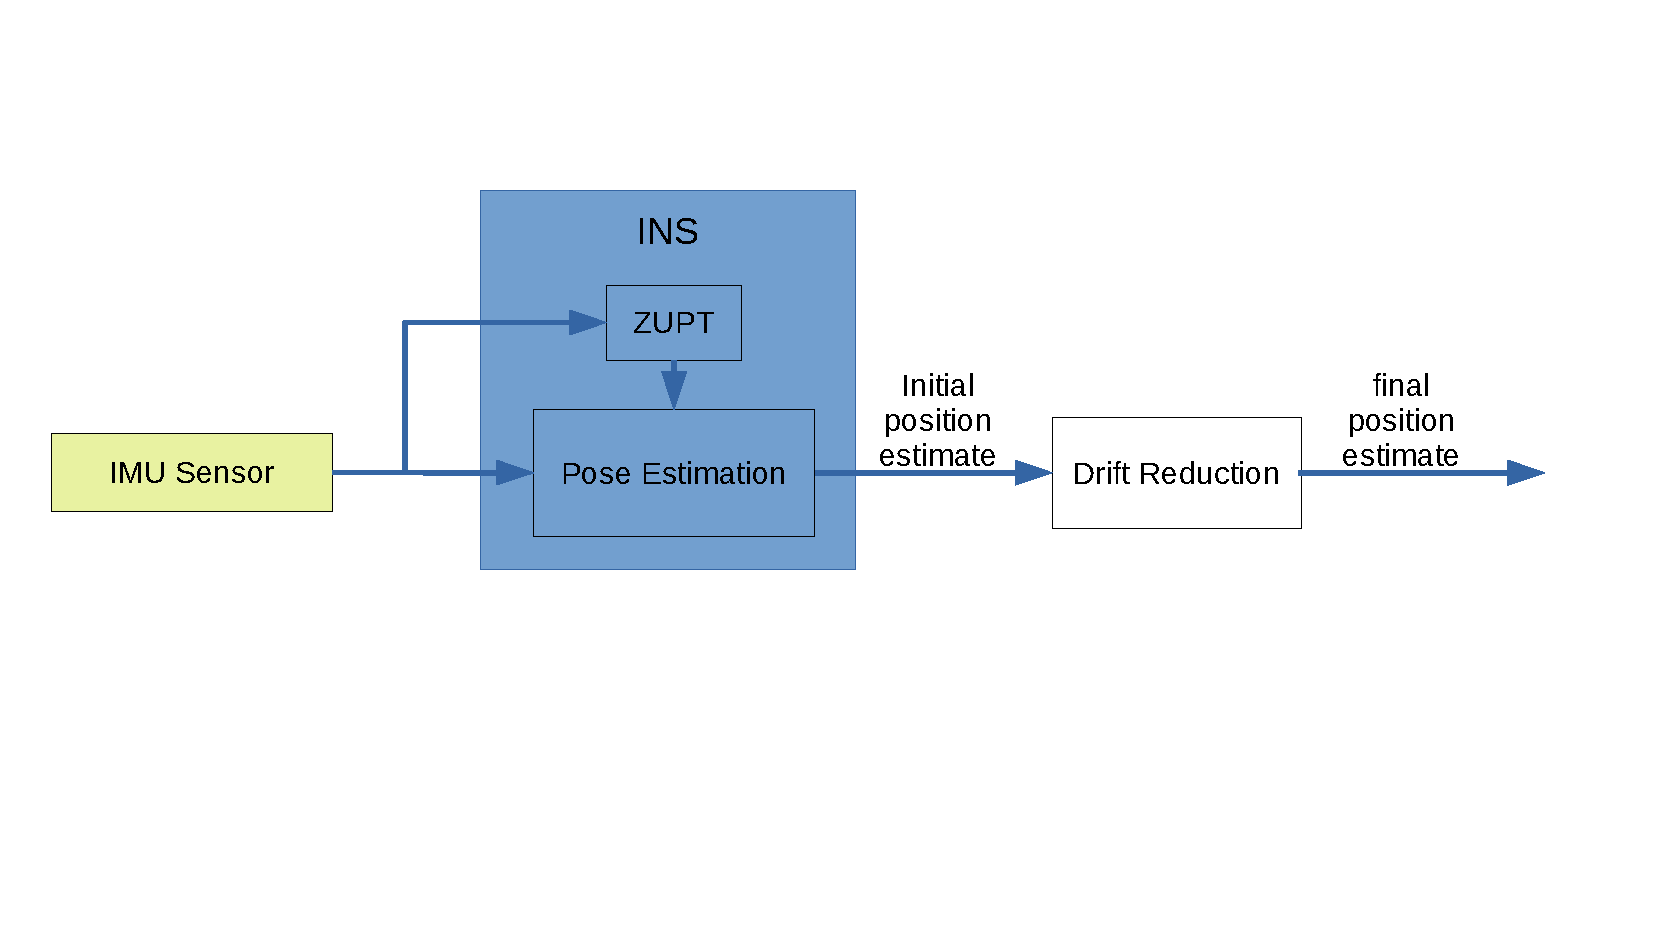
\includegraphics[trim=20 140 290 80, clip, width=0.8\linewidth]{images/INS_diagram}
	\caption{\ac{INS} pedestrian dead reckoning}
	\label{fig:ins_diagram}
\end{figure}
An Inertial Navigation System, as seen in \cref{fig:ins_diagram}, estimates pose, consisting of orientation and position, using sensor fusion algorithms. These methods are directly applied to the signals generated by MEMS IMU sensors \cite{Wu2019}. Examples of sensor fusion algorithms are the Extended Kalman Filter (EKF) and Complementary Filter (CF) \cite{Kok2017}. Sensor fusion algorithms can estimate position and orientation by integrating acceleration twice and integrating angular velocity once, respectively. This integration, in combination with the effects of noise and bias found in MEMS IMU, causes estimation errors to grow cubically with time for INS \cite{Harle2013}. \par

A technique frequently used to compensate for the built-up error in INS is zero velocity update (ZUPT) and zero angular update (ZARU) \cite{Harle2013}. It utilizes the ability to detect time periods in which the sensor is stationary during locomotion. Once detected, ZUPT uses the assumption that speed and angular velocity are zero at that time moment \cite{Wu2019,Harle2013}. this a form of pseudo-measurement. This is because the stationary phase is detected, with zero angular and linear velocity being implied by the assumption, which is not an actual measurement. Comparing the assumption with the output of the sensor fusion algorithm, an error can be calculated and used to compensate for the sensor fusion estimate. This process is generally known as a measurement update and can occur every time a stationary period is detected.  Through this form of measurement update the error grows linearly with number of steps \cite{foxlin2005pedestrian}.\par

Detecting brief stationary time periods in pedestrian IMU data is done easiest when the sensor is placed on the foot \cite{Diez2018,Davidson2017}. This is because a stationary period is much more pronounced in accelerometer data when the sensor is placed there \cite{Yu2019,Wu2019}.  When walking, a foot periodically returns to an actual stationary state and stays there for a brief period of time, approximately 0.1 to 0.3 seconds \cite{Ren2016a}. This has lead to most \ac{INS} research being foot-sensor based \cite{Diez2018,Wu2019}. A recent deviation from this trend, \citet{Solin2018a} overcome this preference for a foot-based system with a combination of several different pseudo measurements, loop closure, and position fixes, opening up new possibilities for implementing INS in non foot based use cases.\\
%The highest accuracy in PDR has been reached with INS in combination with ZUPT \cite{Hardegger2012}.

% Considering this, a focus will be put on implementing a SHS with the potential to handle different carrying modes.
\section{Step and Heading System}
\label{sec:rw-SHS}
\begin{figure}[H]
	\centering
	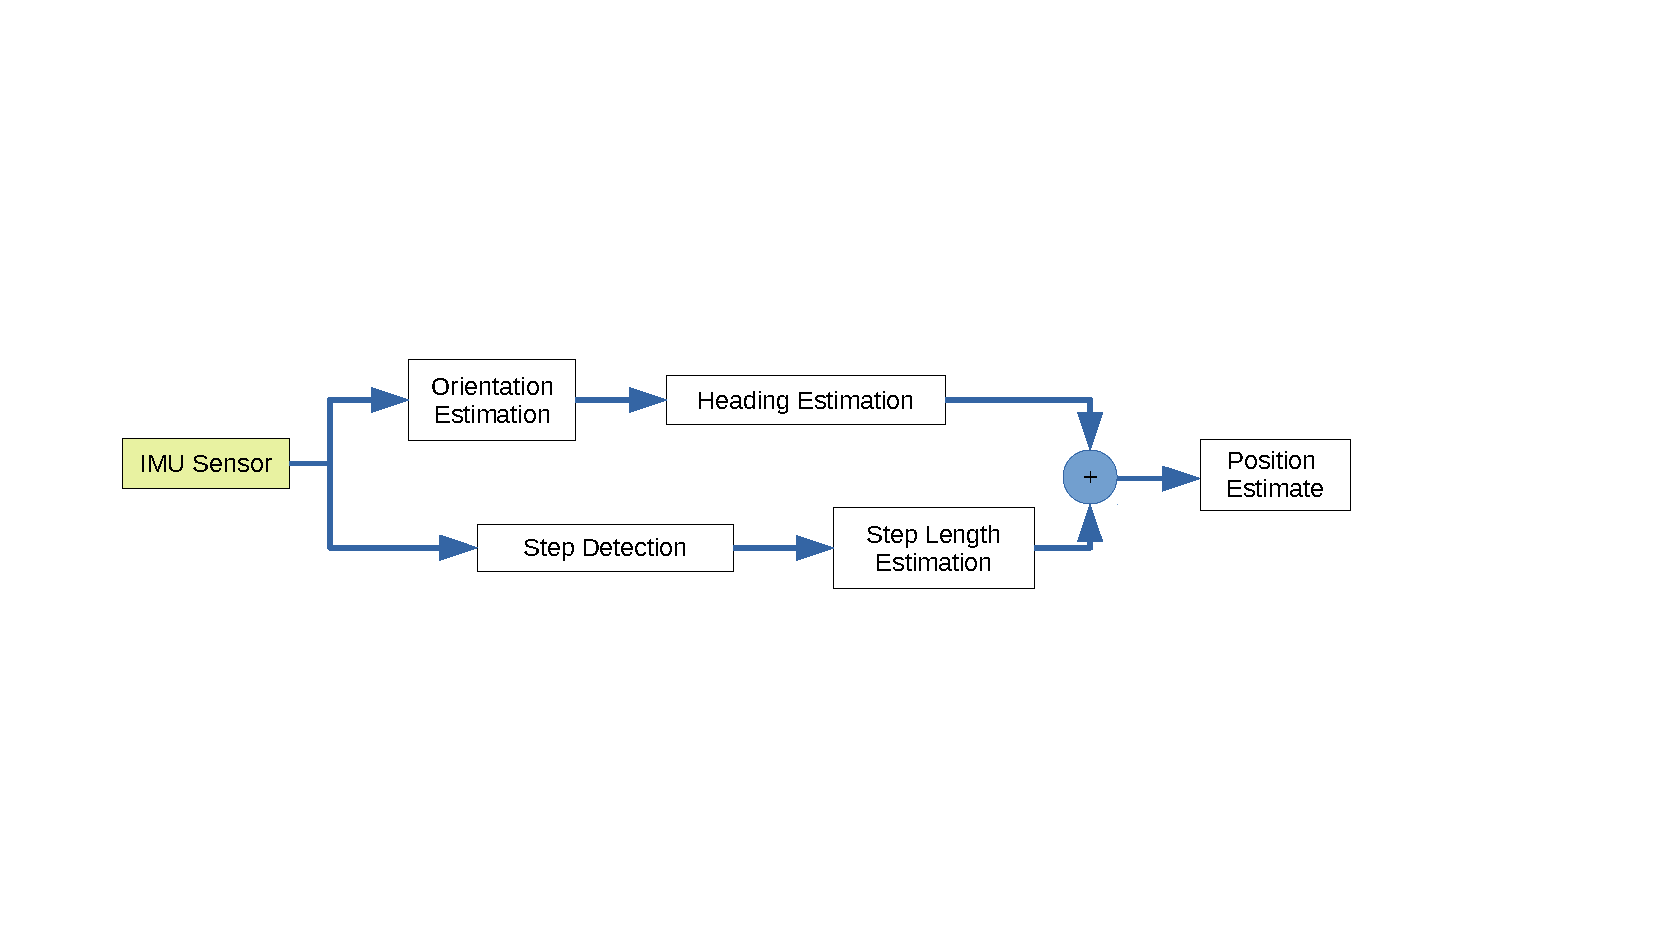
\includegraphics[trim=40 120 180 80, clip,width=\linewidth]{images/shs_diagram}
	\caption{\ac{SHS} pedestrian dead reckoning}
	\label{fig:shs_diagram}
\end{figure}
A step and heading system, as shown in \cref{fig:shs_diagram}, is a form of dead reckoning that detects steps, estimates step length, and the heading in which the pedestrian is moving. This position estimation can be represented by \cite{MunozDiaz2019}
\begin{equation}
	\label{eq:SHS_dynamic_model}
	\left(\begin{array}{l}
		x_t \\
		y_t
	\end{array}\right) 
	=
	\left(\begin{array}{l}
		x_{t-1} \\
		y_{t-1}
	\end{array}\right) 
	+l_{t} \left(\begin{array}{l}
		\cos \left(\theta_{t}\right) \\
		\sin \left(\theta_{t}\right)
	\end{array}\right)
\end{equation}

where $x_{t}$  and  $y_{t}$ represent the position in the $x$-axis and $y$-axis at time  $t$, respectively. $l_{t}$ stands for the step length, while $\theta_{t}$ is the step heading of the pedestrian at time $t$.
Similarly to INS with ZUPT measurement updates, SHS position error is proportional to the number of steps taken. The largest difference is that this error growth does not have a preference of using foot-based sensors, allowing for other sensor placements \cite{Diez2018b}. However, other of sources of error can be introduced due to errors in the detection of steps and their length estimation.  Since other sensor placements are possible, SHS is the PDR technique often used with smartphones as the base for sensing [\qn]. 

%This indicates that this technique is appropriate for further investigation in answering the thesis research questions.\\

%This method can be combined with a particle filter \cite{Koivisto2016, Jackermeier2018}. This allows for more constraints, consequently requiring less particles for localization.
\section{Drift Reduction through Map Information}
PDR methods alone accumulate error with time and are therefore not ideal for long-term pedestrian tracking \cite{Hardegger2012}. Drift reduction methods can be used to try and compensate for this error \cite{MunozDiaz2019a}.  These methods use additional information to restrict the possibilities in which the position estimate can be. One approach is by complement the solution with the infrastructure dependent solutions that require external signal generation \cite{Gu2019}. Another source of information is spatial context \cite{Gu2019}. This includes maps, spatial models and landmarks.

\subsection{Landmark Detection}
A map describes the indoor layout of building, often in the form of of a floor plan \cite{Gu2019}. Using maps assumptions or simplification to restrict the movement. Examples include restricting the movement to be parallel to the outer walls of a building \cite{Abdulrahim2011}. Another is representing the indoor environment as a set of links and nodes, along which the position estimate can move \cite{Davidson2017,Jackermeier2018} 
One approach to drift reduction is through the use of landmark detection. Landmarks are locations with a unique footprint detectable in sensor data. When the user visits a landmark and this is detected, the location of the landmark can be used to calibrate the position estimate of the user, hence compensating drift \cite{Diaz2017}. In addition to drift reduction by position comparison, landmark detection can also be used in determining the user specific parameters of \ac{SHS} online, such as step length estimation parameters \cite{Gu2019,Shang2015}.  Depending on the sensors available, different landmarks become detectable. Examples of landmarks are doors and stairs \cite{Diaz2017,Gu2019,Torok2014}, but also unique magnetic footprints \cite{MunozDiaz2019}, and electromagentic signal footprints \cite{Gu2019}. Some landmarks can be easily determined beforehand, through the use of available building blueprints \cite{Gu2019}. Others can be detected online \cite{Hardegger2012, Hardegger2016}, not requiring a map representation to be available beforehand, using technique such as \ac{SLAM}. 

One form of landmark detection can be done through activity recognition. \\
\textcolor{cyan}{above section can be smoother} \\ \newline
\textcolor{cyan}{ I need to refer to the use of particle filters and that for PDR their use is two fold, landmark detection and absolute position estimate}

\subsubsection{Activity Recognition}
Activity recognition is large research field in which methods span a broad range of complexity, from simple thresholding to the use of deep learning techniques such as neural networks and its many variations \cite{Lima2019}. Even the subset of activity recognition that use IMU sensors does not decrease the amount of possibilities significantly.

%TODO add drear as activity recognition

The choice for a particular activity recognition method is often a trade-off between performance and computational complexity \cite{Bulling2014}. Considering the scope of this thesis, certain constraints can be applied, such as that the system should be able to function on a smartphone and must use comparable sensors to those found in such devices, thus MEMS IMUs. \citet{Shoaib2015} have performed an extensive survey that focuses on the online activity recognition solely using mobile phone sensors and onboard processing. Other metrics such as resource consumption were also presented. 30 papers were found to meet the requirements of the review. Within the review they indicate that most commonly used classification methods include Decision Tree, support vector machine (SVM), K-nearest neighbor (KNN) and Naive Bayes, in descending order. A third of the papers were found to use decision trees. All but 6 of the papers had the training process occurring offline. The classification process takes the method generated offline, and uses it online to classify new activities. The authors refrain from listing any performance measures, such as accuracy or precision, since no direct comparison between the different methods is made. \citet{Ahmad2020} specifically focuses on seeing whether smartphone activity recognition techniques are also applicable to smartwatches, and what parameters, including classifiers, work best. Activities to recognize included walking, up-stairs, down-stairs, running, and jogging. Their results indicated that  Decision Trees, SVM and KNN had around 90 percent accuracy a minor difference. \citet{Shoaib2016} show that combining information from both a smartwatch and smartphone, complex human activity recognition is improved compared to when only a smart watch is used. 

\subsection{Particle Filter}
\label{sec:method-pf}
In order to counter estimate drift,  map information can be used in combination with a Particle Filter. This is a numerical Bayes estimator able to estimate non linear posterior densities, allowing for multimodal distributions \cite{gustafsson2010particle,kihlberg2012map}. Multimodal distribution refers to distributions with multiple maxima in the probability density function. This allows the particle filter to have multiple hypothesis for the system that it is modeling. In the case of localization, it may therefore indicate that there are two position estimates are equally as likely based on the information that the filter has received so far. This can occur due to symmetry in the indoor environment \cite{Woodman2008}. \\
The particle filter is known to work well in three dimensional state space \cite{gustafsson2010particle}, with higher dimensions making the particle representation too sparse to be a meaningfully represent the posterior distribution. Since for indoor localization only y position, x position and heading are needed, the particle filter is sufficient.
\par
As the name suggests, the particle filter uses a finite amount of particles to determine a state estimate. These particles are weighted and are propagated through a motion model, augmented with a noise realization on relevant variables. These noise realizations represent uncertainty of certain components of the motion model. The probability density function of these noise realizations are defined beforehand. Taking the weights of each particle into account a prior estimate can be made. \par 
Measurement updates are used to calibrate the particles throughout their trajectory. These measurements may come from different sources, including map information and landmark detection. When a measurement occurs the particle cloud is compared with the measurements, adjusting the individual weights accordingly. This process is familiar to the reader as it closely resembles that of the previously mentioned Kalman Filter, also a Bayes estimator.\par

\citet{Harle2013} can help limit drift and absolute position estimate

\begin{enumerate}
	\item \textbf{Measurement update} \\
	Each particle is weighted against constraints or system evaluation function. The likelier the particle is within the system constraints, the higher the weighting is. Each particle's weight is redefined through \cref{eq:gen_pf_weight},	where the normalization weight ($c_k$) is given by \cref{eq:gen_pf_probability density}.
	Here $\omega^i_k$ is the weighting for particle $i$ at time $k$, $y_k$ is the measurement at time $k$,  and $N$ is the total number of particles.
	
	\item  \textbf{Estimation} \\
	Using the weightings and positions of the particle cloud, an estimate can be made of the posterior probability density of the process that is being modeled  \cite{gustafsson2010particle}. There are different ways of defining the eventual position estimate. The maximum a posteriori (MAP) estimate picks the particle with the highest weight from the posterior probability function \cite{Saha2009}, while the  minimum mean square error (MMSE) estimate calculates a weighted mean \cite{gustafsson2010particle,Saha2009} as in \cref{eq:gen_pf_estimation}.
	
	\item \textbf{Resampling} \\
	Depending on the new weights of the different particles, a subset is taken and resampled to form a new set of particles, which will be used in the next iteration of the particle filter.
\end{enumerate}

%\begin{algorithm}[H]
%	\SetAlgoLined
%	\caption{Bootstrap Particle Filter}
%	\label{algo:bootstrap_PF}
%	choose the number of particles N.\\
%	% choose a proposal distribution $ q(x_{k+1}|x_{1:k},y_{k+1})$, resampling strategy and the number of particles N.\\
%	% \KwResult{Write here the result }
%	\underline{initialization:}
%	Generate 
%	\begin{subequations}
%		\begin{equation}
%			x^i_1 \sim p_{x_1},
%		\end{equation}
%		and let
%		\begin{equation}
%			\omega^i_{1|0} = 1/N.
%		\end{equation}
%	\end{subequations}
%	\;
%	\For{k = 1,2,...}{
%		\underline{measurement update:}\\
%		\begin{subequations}
%			
%				
%				\begin{equation}
%					\omega^i_{k|k} = \frac{1}{c_k} \omega^i_{k|k-1} p(y_k|x^i_k),
%			\label{eq:gen_pf_weight}	
%			\end{equation}\\
%				where the normalization weight is given by
%				\begin{equation}
%					c_{k}=\sum_{i=1}^{N} w_{k | k-1}^{i} p\left(y_{k} | x_{k}^{i}\right)
%					\label{eq:gen_pf_probability density}
%				\end{equation}
%			
%			\underline{estimation:}\\
%			\begin{equation}
%				\hat{x}_{k | k} =\sum_{i=1}^{N} w_{k}^{i} x_{k}^{i}.
%				\label{eq:gen_pf_estimation}
%			\end{equation}
%			\underline{resampling:}\\
%			take $N$ samples with replacement from the set $\{x^i_{1:k}\}^N_{i=1}$ where the probability to take sample i is $\omega^i_{k|k} = 1/N$.\\
%			\underline{time update:}\\
%			Generate predictions according to the dynamic model, using realizations of the process and measurement noise.
%			\begin{equation}
%				\label{eq:PF_dynamic model}
%				x_{k+1}^{i} \sim p\left(x_{k+1}^{i} | x_{k}^{i}\right)
%			\end{equation}
%		\end{subequations}
%		
%	}
%\end{algorithm}


\section{SHS Components}
\subsection{Walk and Step Detection}
\label{sec:rw - step detection}
Walk detection is determining from sensor data whether a walking activity is being performed. Step detection is deciding when during the walking activity a step is taken. \\
Techniques such as feature classification, frequency domain analysis, and time-domain thresholding can be used to detect the two activities \cite{Yang2014}. An overview of techniques  is  shown in \cref{fig:step_detection_options} and summarized in \cref{tab:step_detection_comparison}. %The reader is referred to \cite{Brajdic2013} for a detailed explanation of each solution.

Naturally, each form of analysis for walk and step detection has its advantages and disadvantages.\\
Time-domain analysis often uses the acceleration norm, making it robust to sensor orientation \cite{Davidson2017}. Its simplest form, thresholding, is trivially simple to implement. The problem with thresholding is that it is difficult to determine the optimal value, as it can vary between users, surfaces, and even shoes \cite{Brajdic2013}. \\
Similar to time-based methods, the periodicity in the norm of acceleration during locomotion is frequently invariant to sensor placement. This therefore also makes frequency analysis robust to sensor orientation. Frequency methods have the disadvantage that they are only able to detect periodic motion. 
For both frequency and time domain-based analysis, it is possible that certain motions, aside from the desired motion, can cross the threshold and generate false positives. In addition, frequency analysis and template matching, a more advanced time based method, will have a certain computational overhead to consider \cite{Davidson2017, Harle2013}. \\
Feature classification methods use features in accelerometer traces to classify steps, using form of machine learning. These method have the advantage that they can determine relations from labeled data automatically, removing a need for humans to define them. This is also a disadvantage as it requires labeled data, the gathering of which can be a labor-intensive process \cite{Bulling2014}. Furthermore, the relationships they determine will depend on the data gathered. This may lead to person dependent performance [\qn]. In addition, certain classification methods may require significant processing power, limiting the platforms on which it can perform [\qn].


\begin{figure}
	\centering
	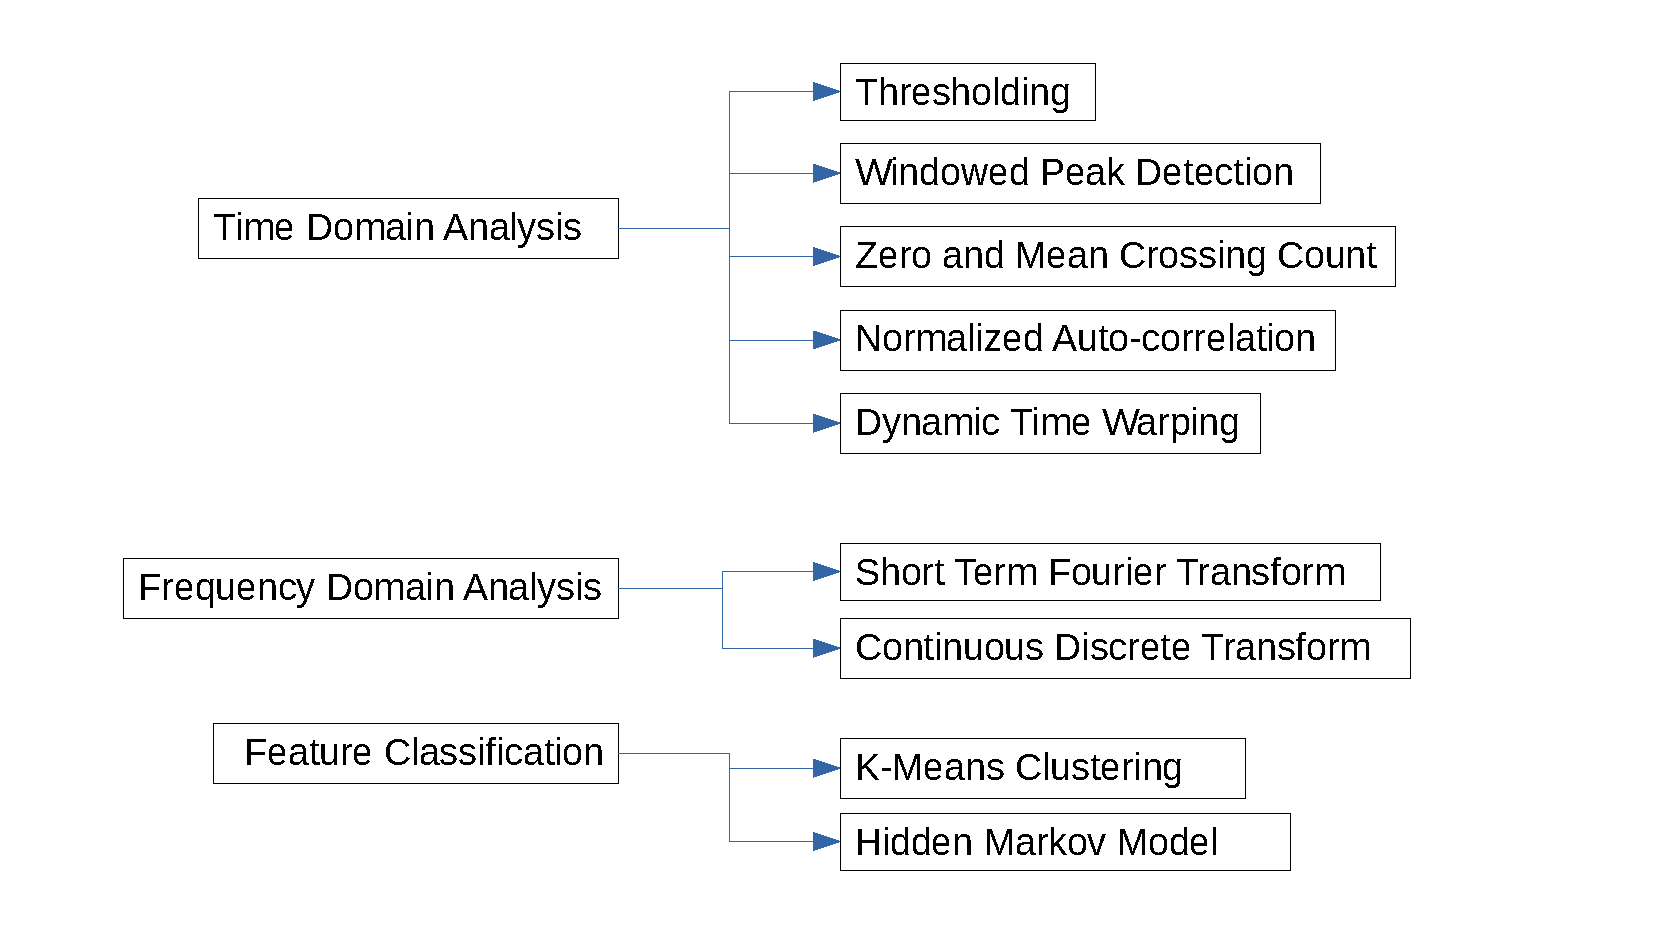
\includegraphics[trim=0 15 0 20, clip,width=0.7\linewidth]{images/step_detection_options}
	\caption{Overview of walk and step detection methods}
	\label{fig:step_detection_options}
\end{figure}

	\begin{table}
	\centering
	\footnotesize
	\begin{tabularx}{\linewidth}{@{} P{17mm} L}
		\toprule
		\thead[lb]{Technique}	&   \thead[c]{Explanation}	\\
		\midrule			
		Threshold & Acceleration magnitude is monitored for the passing of certain values or sign changes, in the case of Zero Crossing method \cite{Davidson2017,Harle2013}. Typically determines when the foot is on the floor \cite{Harle2013}, but has also been applied to pitch angle of the upper leg, where the sensor has been placed \cite{Diaz2014a}. In some instances, the thresholds are altered adaptively, for example through different motion mode detection or information gathered from the previous step \cite{Wu2019}.\\ \cline{1-2}
		(Windowed) Peak Detection & Recognizes local maximum or minimum on acceleration magnitude caused by foot impact on the floor, often within a sliding window \cite{Susi2013}. Generally combined with thresholding, which is one of the simplest combination used with \ac{SHS} \cite{Davidson2017}. \\ \hline
		Auto-correlation (Template Matching) &  Finds correlation of a signal with a time-shifted copy of itself. It leverages the strong cyclic nature of bipedal locomotion \cite{Harle2013}. Since the lag for the highest correlation is not known beforehand, an interval is often swept and correlation values compared. \\ \hline
		Dynamic Time Warping & Similar to autocorrelation, it measures the similarity between two waveforms from accelerometer data \cite{Davidson2017}, These waveforms can both come from the data or one could be a stride template generated offline. A non linear mapping between the two methods is made, resulting in a DTW distance. A smaller distance indicates higher similarity \cite{Davidson2017}.  \\ \hline
		Short Term Fourier Transform & Transforms acceleration signal of successive windows of data into the frequency domain. For spectral analysis, a subset containing a stride (two steps) is required to determine the frequency \cite{Harle2013}.  \\ \hline
		Wavelet Decomposition & Acceleration magnitude is split into low and high-frequency components, from which the dominant frequency is assumed to be the walking frequency. Iterating this process on the resulting low-frequency signal approximation, a smoother shaped dominant low-frequency signal is generated. The frequency of this signal corresponds to walking cadence \cite{Davidson2017}. \\ \hline	
		Hidden Markov Model & Uses gait cycles segmented into different states of a state machine, to determine if a step has been taken \cite{Ren2016a}. Thresholds can be used to induce a state change. If a full state machine cycle is achieved, a step is detected.\\ \hline
		K Nearest Neighbours & Uses labeled data containing features from successive time windows and compares a new time window with its features. It finds the labeled data whose features are most similar. This new set then recieves its label. \\
		\bottomrule
	\end{tabularx}
	\caption{Overview of different step detection methods}
	\label{tab:step_detection_comparison}
\end{table}

In \cite{Brajdic2013}, a variety of algorithms for both walk detection and step detection on unconstrained smartphones are tested and compared. The paper reviews techniques with different levels of complexity from a variety of different papers. In order to compare the different techniques, \citet{Brajdic2013} collected a large dataset from 27 test subjects leading to 130 recordings was made. Each subject held the smartphone in six different carrying modes: in hand in front of user (idle and with device interaction), in a front pocket, in a back pocket and in a handbag or backpack. A ground truth was generated by video recording each session and manually counting the amount of steps taken. Using this dataset a comparison is made between the nine algorithms.
\newline
The paper concludes that for the generated dataset, the best step counting results were obtained using the windowed peak detection, hidden Markov model, and continuous wavelet transform. Each had a median error of about 1.3\%.\\
Considering the relative simplicity of the technique, the authors recommend that windowed peak detection as the most efficient algorithm for step detection. The best walk detection algorithms were thresholds on either standard deviation or signal energy,  short-term Fourier transform, and normalized autocorrelation.\\
\citet{Salvi2018} build upon the conclusions and recommendations of \citet{Brajdic2013}, with the aim of further optimizing the windowed peak detection algorithm and its parameters. The algorithm is based on the approach of \citet{Palshikar2009} and consists of 5 stages run in series. These are pre-processing, filtering, scoring, detection and post processing. An exhaustive grid search across the parameter space was performed to find the optimal set for step detection. Using these parameters, an average accuracy of $95\% \pm 4.5\%$ was reached for the different carrying modes. 

%These results make this approach 


\subsubsection{Step Length Estimation}
In order to generate a displacement vector from step detection, the step length must be estimated. \citet{Collins2013a} found that increasing step speed leads to larger step lengths, while step speed can have slow and spontaneous fluctuations depending on the motion mode. In addition, step size depends on the physical characteristics of the user and on their walk strategy, which can be different per individual \cite{Diez2018}. These discrepancies indicate that using a simple average step length for every pedestrian could result in quick accumulation of error. 

\citet{Diez2018} categorizes step length estimation methods into integration based and model-based methods. \\
Theoretically, the double integration of the IMU acceleration signal is the best approach to step size estimation, using the INS approaches outlined in chapter \secref{sec:INS}. This would give a direct measurement of displacement. It does not require any modeling, assumptions, or person-specific calibration \cite{Diez2018}. However, since it would be an INS approach, it suffers from the same drift problems and would require the same solutions. Therefore this approach benefits from having the sensor to be located on the foot. \\
Analytical models can be made of human mobility based on geometrical relationships of body composition, angles, and displacement of body parts. One of the largest disadvantages of a model-based approach is that human proportions are not uniform, requiring approximations and/or some form of calibration for the model to be accurate.
An overview of different step length estimation methods can be found in \cref{tab:step_length_methods}.

\begin{table}[H]
	\centering
	\textcolor{cyan}{Table with different step length methods}
	\caption{Different Step Length Methods}
	\label{tab:step_length_methods}
\end{table}

\citet{Vezocnik2019} compared different existing step length estimation algorithms. The review focuses on the methods applicable to smartphone use. This means methods that do not require training and do not require the sensor to be placed on the foot. This, therefore, excludes machine learning and INS systems. The models used are either based on an inverted pendulum model or relate predictors to step length. Examples of step length predictors are step frequency and acceleration range within a step. The robustness of the methods was tested by having the smartphone in different carrying modes. This includes front 

\begin{equation}
	\label{eq:Tian2016_sle}
	\text{step size} = K \cdot h \cdot \sqrt{F}.
\end{equation}

Here $K$ is a tunable parameter, $h$ is the height of the user and $F$ is the step frequency. This method reported an average error of  4.59 \% for personalized variables and 6.96 \% for global ones. For personally tuned variables the method of \cite{Weinberg2002} was best. This is an inverted pendulum model in which the human center of mass is used, located approximately at the pelvis. The center of mass rotates as an inverted pendulum when taking a step. This is followed by a forward horizontal displacement when both feet are on the ground \cite{Diez2018}. The model is defined as 

\begin{equation}
\text{step size} =K \sqrt[4]{A_{\max }-A_{\min }}.
\label{eq:weinberg_stepsize}
\end{equation}

Here $A_{\max}$ is the largest measured acceleration measured within a step interval, while $A_{\min}$ is the smallest. $K$ is a calibration variable  \cite{Weinberg2002,Diez2018}. The model had an average error of  10.64 \% for global variables and  3.60 \% for personalized \cite{Vezocnik2019}.



\subsubsection{Step Heading Estimation}
Step heading determines the direction of a detected step. It requires the orientation of the sensor in the navigation frame and determining in what direction the sensor is moving in the sensor frame. This provides an estimate in which direction the sensor is moving in the navigation frame.  Step heading estimation is currently the component within SHS whose performance is the most limiting for positioning purposes \cite{Diez2018b, Qian2013,Combettes2017}.\\
Even though the phone orientation may be known accurately, the direction in which the user is moving is not instantly clear. \par
There are two approaches to determining the heading. The first is knowing beforehand what the orientation of the phone is with respect to heading \cite{Tian2016}.  This would constrain the carrying mode that can be used.  With the use of motion classification, this method could be expanded, where different carrying modes can be sensed,which changes the heading accordingly. Heading per carrying mode would need to be derived beforehand, through the training of the necessary model. 

\textcolor{cyan}{this section is not done yet, and so will need completing } \\ \newline
\textcolor{red}{I do not have a comparison of different orientation estimation methods. How do I explain the use of EKF compared to the different possibilities? Should i just add this comparison section?}

\subsubsection{Activity Recognition}





% The Beauregard implementation introduced backtracking, whereby the filter kept a limited history of each particle’s ancestors to allow deletion of an entire trajectory when a particle was killed due to a wall constraint. This is a variant of backward belief propagation also used by Rai et al. [23] and is useful to improve position estimates made in the past when live positioning is not a requirement.

\chapter{Method}
\label{chap:method}
In the previous chapter different indoor localization methods were introduced. From this information an initial system design was destilled. The details of the different components can be found in the following sections.

\section{Proof of Concept System Overview}
Summarizing the information and the decision made so far, the overall proof of concept can be found in \cref{fig:system_design}.
\textcolor{cyan}{further explanation}

\begin{figure}[H]
	\centering
	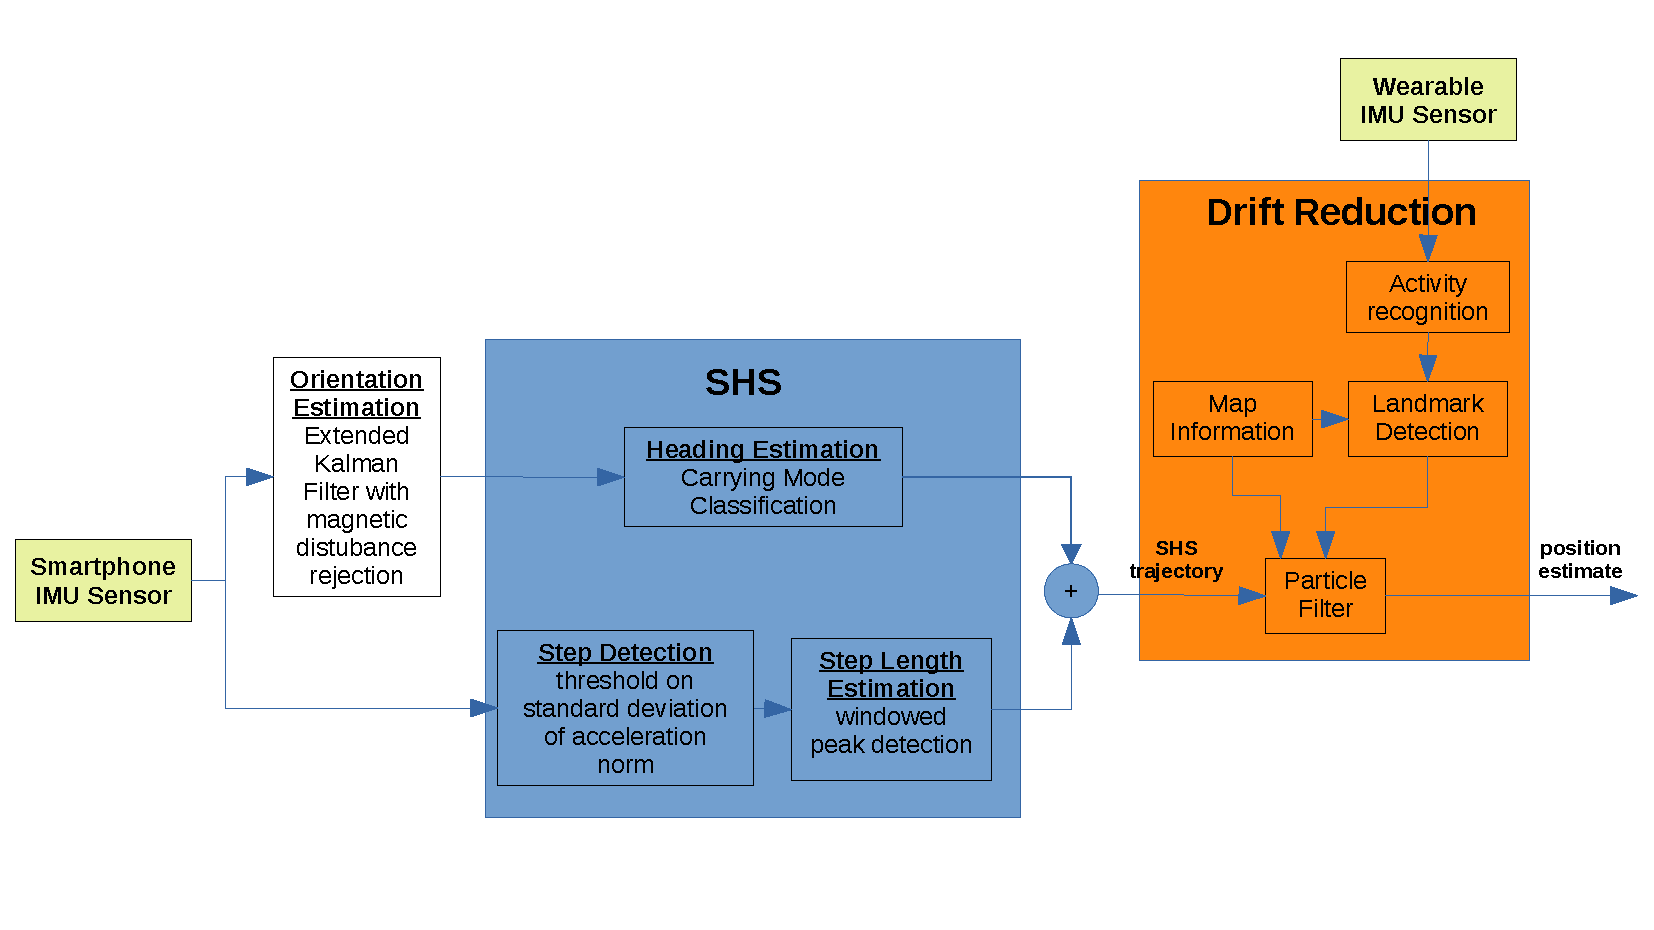
\includegraphics[width=\linewidth]{images/system_design}
	\caption{Overview of proof of concept SHS-PF with activity recognition from wearable device}
	\label{fig:system_design}
\end{figure}


\section{Step Detection and Step Length Estimation}

\textcolor{cyan}{introductory text}

\subsection*{Step Detection}
\label{sec:meth - step detection}
The method used for step detection is similar to the one presented by \cite{Salvi2018}, introduced in \secref{sec:rw - step detection}. 
 An overview of the different components of this windowed peak detection method is shown in \cref{fig:step_detection} . To optimize the algorithm, different combinations of stage components were compared in \cite{Salvi2018}. A custom made, electronic ground truth device was worn by test subjects for easy comparison with the different parameter settings. A dataset of 36 recordings was made,  where three researchers walking for two to three minutes with the phone held in six different carrying modes. This includes in hand, in a front pocket, in a back pocket, in an armband, in a shoulder purse, and in a neck pouch on a string. Each set contains around 2.5 minutes of accelerometer and ground truth data.
\begin{figure}
	\centering
	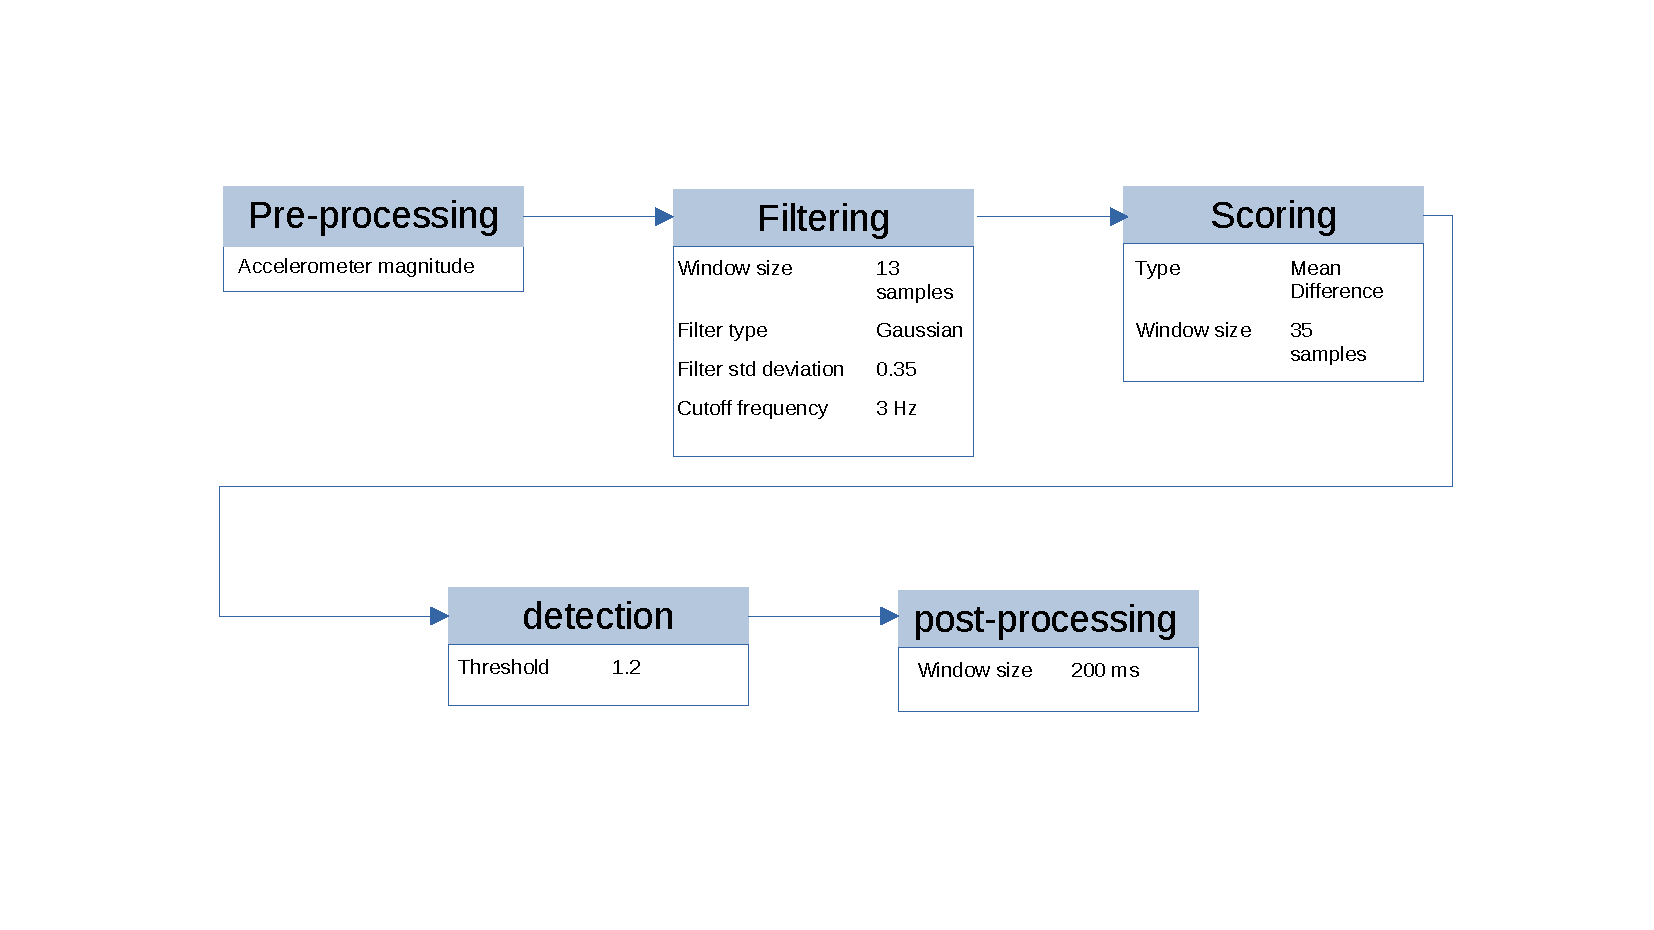
\includegraphics[trim=20 100 50 80, clip, width=0.7\linewidth]{images/step_detection}
	\caption{Windowed peak detection components and parameters used by \cite{Salvi2018}}
	\label{fig:step_detection}
\end{figure}

 This thesis uses the method and parameters found by \citet{Salvi2018} as basis for step detection. The eventually implemented method differs slightly from the referenced paper in that the data is being handled offline, not having to wait for data buffers to fill. It also differs in that it adds the walk detection method from \cite{Brajdic2013}. The values used for the different parameters are based on those found by \cite{Salvi2018}. The implemented method consists of five steps:
\begin{enumerate}
	\item \textbf{Pre-processing} \\
	The IMU used in most smartphones provide acceleration information over three orthogonal axes. For the step detection algorithm the magnitude of the combined signal from the three orthogonal axes is used.
	
	\item \textbf{Walk detection} \\
	Since a person is not walking continuously, the regions in which it does occur need to be indicated. \cite{Brajdic2013} determined that thresholding on the standard deviation of the norm the accelerometer signal was sufficient. This is done using the parameters found by the paper, which is determining the standard deviation over a moving frame of 0.8 seconds, with all standard deviation magnitude levels above $0.6 m/s^2$ being considered walking.
	
	\item \textbf{Filtering} \\
	A gaussian window is applied with a window size of 13 frames and a standard deviation of 0.35.
	
	\item \textbf{Scoring }\\
	With the scoring stage the "peakiness" of a given sample is evaluated. The result
	of this stage should increase the magnitude of any peaks. This makes it easier for the subsequent peak detection. The scoring used is that of mean difference 
	\begin{equation}
		p_{i}=\frac{\sum_{k=-N, k \neq i}^{N}\left(x_{i}-x_{i+k}\right)}{2 N}
		\label{eq:mean difference}
	\end{equation}
	where $p$ is the score given to the sample, $i$ is the index of the sample, $N$ is window size, and $x$ is the sample value.
	
	
	\item \textbf{Step detection} \\
	Here outliers are statistically detected. The algorithm processes the signal by calculating a running mean and standard deviation.
	These two measures determine whether a sample is an outlier or not. If the difference between sample and mean is over 1.2 times the standard deviation, then it is marked as a potential step.
	
	
	\item \textbf{Post-processing} \\
	The final stage of step detection is determining local maxima of the outliers detected in the previous stage. Here local maxima are found that have a minimum separation duration of 0.2 seconds.
	
\end{enumerate}

\begin{algorithm}[]
	\SetAlgoLined
	\caption{Step Detection}
	\label{algo:step_detect}
	\underline{initialization:}\\
	\For{k = 1,2,...}{
		\underline{measurement update:}\\		
	}
\end{algorithm}

The parameters used for the process coincide with those found by the researchers, an overview of which can be found in \cref{tab:parameters_used}.

\begin{table}
	\centering
	\footnotesize
	\begin{tabular}{clc} 
		\hline
		Stage & Parameters & Value \\
		\hline & Window size & $\mathrm{M}=13$ \\
		Filtering & Filter type & Gaussian \\
		& Filter SD & 0.35 \\
		\multirow{2}{*} { Scoring } & & \\
		& Type & Mean Difference \\
		& Window size & $N=35$ \\
		Detection & Threshold & 1.2 \\
		Post-Processing & $t_{\text {window}}$ & $200 \mathrm{ms}$ \\
		\hline
	\end{tabular}
	\caption{Parameters used in \cref{algo:step_detect}}
	\label{tab:parameters_used}
\end{table}

An example of this step detection method and its different stages can be found in \cref{fig:all_stages_of_step_detection}.

\begin{figure}[H]
	\centering
	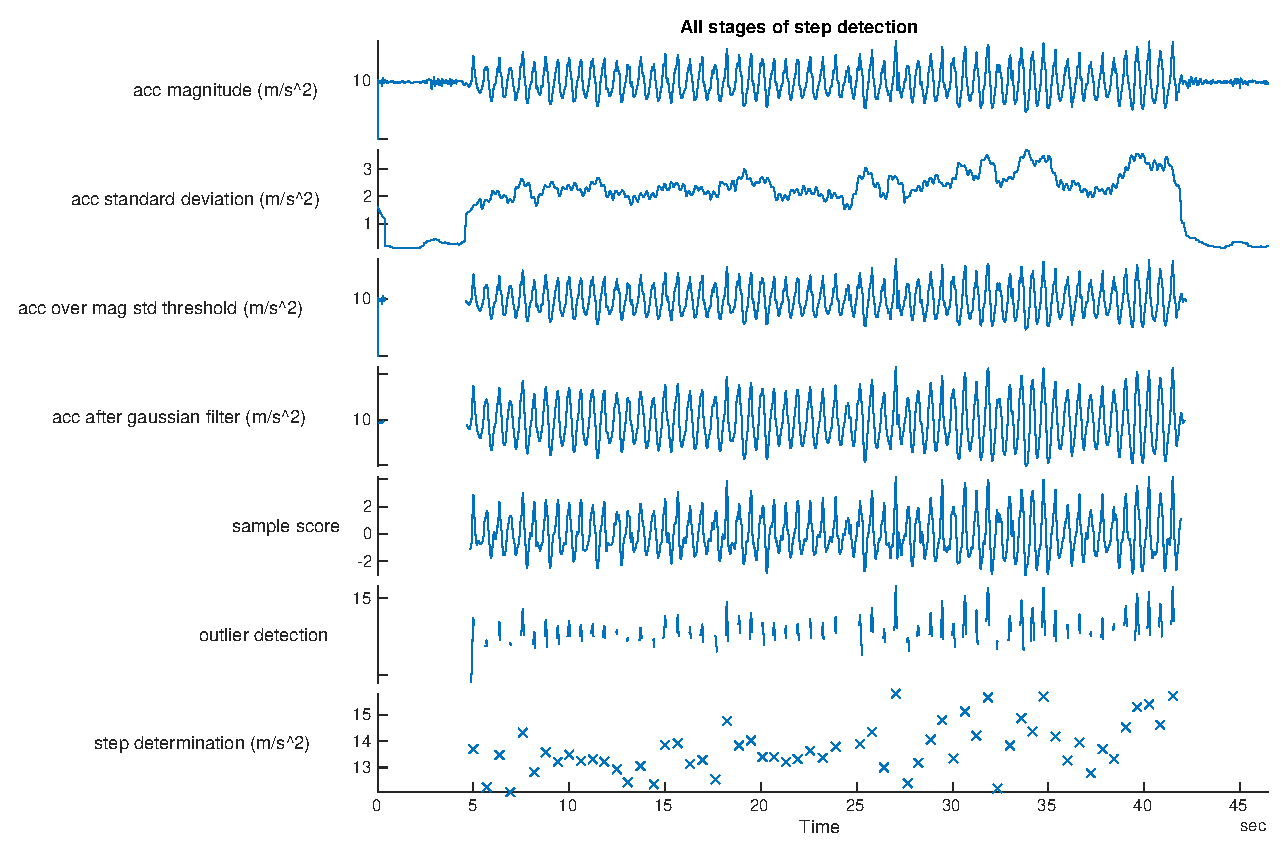
\includegraphics[width=1\linewidth]{images/20200924_1204_All_stages_of_step_detection}
	\caption[All stages of step detection ]{All stages of step detection from recorded accelerometer data, with the x's in the last graph indicating the steps taken }
	\label{fig:all_stages_of_step_detection}
\end{figure}
\subsection*{Step Length Estimation}
For step length estimation the method outlined as working best by \cite{Vezocnik2019} will be used. This is \eqref{eq:Tian2016_sle} in \cref{sec:rw-SHS}. Within this method there is a tuneable parameter that needs to be estimate in order for the method to be applied. One way of doing this is by using the data that \cite{Vezocnik2019} have made available online. Running this data through the above outlined step detection, the result can be used for parameter estimation.

\textcolor{red}{this section is pretty small at the moment, should it require a heading? What else to add?}

\section{Orientation Estimation}
\textcolor{cyan}{introductory text}
\subsection{Coordinate Frames}
Within orientation estimation there are  different coordinate frames to be considered. There are two frames that are of importance for localization: the body frame and the navigation frame.\\
The body frame ($b$) is the coordinate frame of the IMU, the origin of which is at the center of the triaxial accelerometers found in the device \cite{Kok2017}. The navigation frame ($n$) is the geographical frame in which the user is moving. It is also the frame in which we want to determine the pose, consisting of orientation and position, of the body frame. For a localization application it is considered stationary \cite{Kok2017}.
A superscript on a vector is used to indicate in which coordinate frame it is expressed. For example,
$x^n$ is the vector $x$ expressed in the navigation frame. A double superscript on any orientation mapping from one frame to another indicates from which frame to which frame the rotation is occurring. For example,
$R^{nb}$ is a rotation matrix that maps from the body frame to the navigation frame.


\subsection{Orientation Parametrization}
While position is often represented by a point in a 3D orthogonal axis frame, orientation has different parametrizations, each able to map to one another. This chapter will introduce rotation matrices ($R$) and quaternions ($q$), which will be used in the following section to determine orientation from IMU sensor data.

\subsubsection{Rotation Matrix}
Rotation matrices $R \in \mathbb{R}^{3 \times 3}$ have the following properties:

\begin{equation}
	\label{eq:rot_mat_properties}
	R R^{\top}=R^{\top} R=I_{3}, \quad \text { det } R=1.
\end{equation}

These matrices can be used to express a vector $x$ in frame $v$ to frame $u$ as 

\begin{equation}
	\label{eq:rot_mat_rot_x}
	x^{\mathfrak{u}}=R^{\mathfrak{u} \mathrm{v}} x^{\mathrm{v}}.
\end{equation}

Transposing a rotation matrix represent a rotation back to it's original coordinate frame:
\begin{subequations}
	\begin{align}
		\label{eq:rot_mat_trans}
		x^{\mathrm{v}}&=\left(R^{\mathrm{uv}}\right)^{\top} x^{\mathrm{u}},\\
		&=R^{\mathrm{vu}} x^{\mathrm{u}}.
	\end{align}
\end{subequations}

\subsubsection{Quaternion}
A quarternion is a common parametrization of orientation frequently used by attitude estimation algorithms. This is because it is free of non-singularity in attitude representation \cite{Hashim2019}, also known as wrapping. A unit quaternion can be described by

\begin{equation}
	\label{eq:unit_quarternion}
	q=\left(\begin{array}{llll}{q_{0}} & {q_{1}} & {q_{2}} & {q_{3}}\end{array}\right)^{\top}
	=\left(\begin{array}{l}{q_{0}} \\ {q_{v}}\end{array}\right), 
	\quad q \in \mathbb{R}^{4}, 
	\quad\|q\|_{2}=1.
\end{equation}

A rotation of vector $x$ using quaternions between two frames, from $v$ to $u$, is indicated as

\begin{equation}
	\label{eq:quat_rot}
	\bar{x}^{\mathrm{u}}=q^{\mathrm{uv}} \odot \bar{x}^{\mathrm{v}} \odot q^{\mathrm{vu}},
\end{equation}

where $q^{\mathrm{vu}} = \left(q^{\mathrm{uv}}\right)^{\mathrm{c}}$, with the latter representing the quaternion conjugate, defined by 

\begin{equation}
	\label{eq:quat_conjugate}
	q^{\mathrm{c}}=\left(\begin{array}{c}{q_{0}} \\ {-q_{v}}\end{array}\right).
\end{equation}

$\bar{x}^u$ represents the quaternion version of the vector $x^u \in \mathbb{R}^3$, as

\begin{equation}
	\label{eq:quat_vec_ref}
	\bar{x}^u=\left(\begin{array}{l}{0} \\ {x^u}\end{array}\right).
\end{equation}


The $\odot$ operator describes quaternion multiplication, defined by:

\begin{equation}
	\label{eq:quat_multiplication}
	p \odot q=\left(\begin{array}{c}{p_{0} q_{0}-p_{v} \cdot q_{v}} \\ {p_{0} q_{v}+q_{0} p_{v}+p_{v} \times q_{v}}\end{array}\right)
\end{equation}

\subsection{Motion and Measurement Models}
\label{sec:motion_and_measurement_models}
The signals generated by an IMU can be formatted in such a way that orientation can be deduced. For many sensor fusion algorithms this is generally done by defining a motion and measurement model, together forming a state space representation. This state space can be defined as \cite{Kok2017}

\begin{subequations}
	\begin{align}
		\label{eq:orient_dynamics}
		q_{t+1}^{\mathrm{nb}} &=q_{t}^{\mathrm{nb}} \odot \exp _{\mathrm{q}}\left(\frac{T}{2}\left(y_{\omega, t}+e_{\omega, t}\right)\right), 	\\ 
		\label{eq:orient_acc_measure}
		y_{\mathrm{a}, t} &=-R_{t}^{\mathrm{bn}} g^{\mathrm{n}}+e_{\mathrm{a}, t},\\ 
		\label{eq:orient_mag_measure}
		y_{\mathrm{m}, t} &=R_{t}^{\mathrm{bn}} m^{\mathrm{n}}+e_{\mathrm{m}, t}, 
	\end{align}
	\begin{equation}
		\label{eq:orient_ss_noise}
		e_{\omega, t} \sim \mathcal{N}\left(0, \sigma_{\mathrm{\omega}}^{2} \mathcal{I}_{3}\right), 
		\quad 
		e_{\mathrm{a}, t} \sim \mathcal{N}\left(0, \sigma_{\mathrm{a}}^{2} \mathcal{I}_{3}\right), 
		\quad 
		e_{\mathrm{m}, t} \sim \mathcal{N}\left(0, \sigma_{\mathrm{m}}^{2} \mathcal{I}_{3}\right).
	\end{equation}
	\label{eq:orient_state_space}
\end{subequations}

Here \eqref{eq:orient_dynamics} is the motion model and \eqref{eq:orient_acc_measure,eq:orient_mag_measure} are the measurement models. \\
For the motion model, $q^{nb}$ represents unit quaternion from body $(b)$ to navigation frame $(n)$. $T$ is the time period between two samples. $y_{\omega, t}$ is the gyroscope measurement. The $\odot$ operator describes quaternion multiplication, as in \eqref{eq:quat_multiplication}. The $\text{exp}_\text{q}$ operator is defined as

\begin{equation}
	\exp_\mathrm{q} (\eta) = \left(\begin{array}{c}{\cos \|\eta\|_{2}} \\ {\frac{\eta}{\|\eta\|_{2}} \sin \|\eta\|_{2}}\end{array}\right) \label{eq:exp_q_in_text}.
\end{equation}

For the measurement model, $y_{\mathrm{a}, t}\in \mathbb{R}^3$ is the accelerometer measurement and $R^\mathrm{nb}_t$ is the rotation matrix mapped from the orientation quaternion generated in \eqref{eq:orient_dynamics}. $g^n \in \mathbb{R}^3$ is the gravity vector in the navigation frame. Similarly, $y_{\mathrm{m}, t}\in \mathbb{R}^3$ is the accelerometer measurement and $m^n$ is the magnetic field in the navigation frame. \\
This state space model is simplified using certain assumptions.
For both motion and measurement models, the noise terms  $(e)$ is assumed to be normally distributed, independent and have the same noise levels for the three sensor axis of all three sensors, as indicated in \eqref{eq:orient_ss_noise}. The zero mean in these noise definitions also indicate the assumption that the sensors have been calibrated properly and therefore do not contain any bias. \\
Another assumption is that the sensor does not travel over significant distances in comparison to the size of the earth \cite{Kok2017}. Additionally the magnitude of the earth rotation and coriolis acceleration are discarded. Furthermore, it is assumed that the acceleration signal is dominated by the gravity vector, making external acceleration negligible. Additionally, the magnetic field is assumed to be constant. These different assumptions will be needed to taken into account when constructing orientation estimation while walking indoors.

\subsection{Calibration}

For proper orientation estimation, sensor calibration is required. \\
\textcolor{cyan}{elaboration need to introduce the subject} 

%\citet{Moder2017} indicates that it is  beneficial for PDR systems to have the gyroscope and magnetometer bias  calibrated, while the accelerometer bias and scale factor is optional. In addition it is advised to estimate the gyroscope bias frequently before testing.

\subsubsection{Gyroscope Calibration}
Gyroscope measurements from MEMS IMUs are generally offset by a bias ($o_\omega$) and influenced by noise ($e_{\omega, t}$)  resulting in

\begin{equation}
	y_{\omega, t}=\omega_{t}+o_{\omega}+e_{\omega, t},
\end{equation}

where $e_{\omega, t}$ is assumed to have the same noise properties as in \eqref{eq:orient_ss_noise}. The gyroscope bias is slowly time varying but for relatively short experiments can be assumed to be constant \cite{Kok2016}. It can be measured by placing the gyroscope on a flat surface for some time and recording data from the sensor. Since the sensor is not moving, the biases are the means of the data over the three axis and the covariance is the square of the standard deviation of the data to the previously mentioned means.

\subsubsection{Accelerometer and Magnetometer Calibration}
% In outdoor environments, mn is equal to the local earth magnetic field and is accurately
%known from geophysical studies, see e.g. [29]. In indoor environments, however, the local magnetic
%field can differ quite significantly from the local earth magnetic field. Because of that, we treat mn as
%an unknown constant. 

For magnetometer and accelerometer calibration the method outlined by \citet{Kok2016} can be used. This method indicates that for a perfect calibration a magnetometer measures the local magnetic field, no matter the orientation. Any measurement will then lie on a sphere with a radius  equal to the local magnetic field. The same applies for a perfect calibration with an accelerometer, replacing the local magnetic field with the gravity vector. Any sensor calibration should strive to achieve this sphere as best as possible.\\
MEMS sensor are imperfect sensors, with sensor specific errors that can differ per sensor. These errors, including non orthogonality of sensor axis, the presence of zero bias, and difference in sensitivity on different axis \cite{Kok2016} can be combined into a distortion matrix $D$ and offset vector $o$.
This results in the following uncalibrated measurement model,
\begin{equation}
	y_{\mu, t}=D_\mu R_{t}^{\mathrm{bn}} \mu^{\mathrm{n}}+o_\mu +e_{\mu, t},
\end{equation}

where $\mu$ is a placeholder for either the acceleration vector or local magnetic field vector with the superscript indicating in what coordinate frame it is expressed. Each have their own respective distortion matrix and offset vector. $y_{\mu, t}$ represents the measurement associated with either gyroscope or magnetometer.
Due to the distortion matrix and offset vector, the measurements lie on a translate ellipsoid instead of on a sphere as previously stated. Determining these parameters, the sensor errors can be compensated through

\begin{equation}
	y_{\mu, t}^{cal}=D_\mu^{-1}\left(y_{\mu, t}-o_{\mu}\right)
\end{equation}

Without loss of generality the desired sphere radius can be normalized and written as followed to expressed the sphere characteristic
\begin{equation}
	\begin{aligned}
		\left\|\mu^{\mathrm{b}}\right\|_{2}^{2}-1 &=\left\|R_{t}^{\mathrm{bn}} \mu^{\mathrm{n}}\right\|_{2}^{2}-1 \\
		&=\left\|D^{-1}\left(y_{\mu, t}-o-e_{\mu, t}\right)\right\|_{2}^{2}-1=0.
	\end{aligned}
\end{equation}

Since real calibration measurements are still corrupted by noise, the above equality does not hold exactly. The ellipsoid fitting problem can be rewritten as

\begin{equation}
	\label{eq:calib_elipsoid}
	y_{\mu, t}^{\top} A y_{\mu, t}+b^{\top} y_{\mu, t}+c \approx 0,
\end{equation}
where
\begin{subequations}
	\label{eq:calib_elipsoid_components}
	\begin{align}
		A \triangleq D_\mu^{-\top} D_\mu^{-1}, \\
		b \triangleq-2 o_\mu^{\top} D_\mu^{-\top} D_\mu^{-1}, \\
		c \triangleq o_\mu^{\top} D_\mu^{-\top} D_\mu^{-1} o_\mu.
	\end{align}
\end{subequations}

Assuming that $A$ is positive definite, this defines an ellipsoid with parameters $A, b$ and $c$. This can be rewritten as a linear relation as

\begin{equation}
	M \xi \approx 0
\end{equation}
with
\begin{equation}
	M=\left(\begin{array}{ccc}
		y_{\mu, 1} \otimes y_{\mu, 1} & y_{\mu, 1} & 1 \\
		y_{\mu, 2} \otimes y_{\mu, 2} & y_{\mu, 2} & 1 \\
		\vdots & \vdots & \vdots \\
		y_{\mu, N} \otimes y_{\mu, N} & y_{\mu, N} & 1
	\end{array}\right), \quad \xi=\left(\begin{array}{c}
		\mathrm{vec} A \\
		b \\
		c
	\end{array}\right),
\end{equation}

where $\otimes$ is the kronecker product and vec the vectorization operator.
The ellipsoid fitting problem can be written as the following semidefinite program \cite{Kok2016} 
\begin{equation}
	\begin{array}{ll}
		\min _{A, b, c} & \frac{1}{2}\|M\left(\begin{array}{c}
			\operatorname{vec} A \\
			b \\
			c
		\end{array}\right)\|_{2}^{2} \\
		\text { s.t. } & \operatorname{Tr} A=1, \quad A \in S_{++}^{3 \times 3}
	\end{array},
\end{equation}

where $S_{++}^{3 \times 3}$ is the set of $3 \times 3$ positive definite symmetric matrices. This is a convex optimization problem with a globally optimal solution that can be solved using software packages such as CVX \cite{cvx} and YALMIP \cite{Lofberg2004}. Initial estimates of the calibration matrix $D_\mu$ and offset vector $o_\mu$ can be obtained from the estimated $\widehat{A}, \widehat{b}, \widehat{c}$ defined as

\begin{subequations}
	\begin{align}
		\beta &=\left(\frac{1}{4} \hat{b}^{\top} \widehat{A}^{-1} \widehat{b}-\widehat{c}\right)^{-1} \\
		\widetilde{D}_{\mu 0}^{\top} \widetilde{D}_{0} &=\beta \widehat{A}^{-1} \\
		\widehat{o}_{\mu 0} &=\frac{1}{2} \widehat{A}^{-1} \widehat{b}
	\end{align}
\end{subequations}

An example of this calibration can be found in \cref{fig:calibration_magnetometer} where data was recorded by recording a smartphone in as many orientations as possible, in a stationary setting. It clearly shows how the uncalibrated data is mapped to a unit sphere. The distortion matrix and offset vector for this calibration are 

\begin{subequations}
	\begin{align}
	\widehat{D}_{m0} &= \left(\begin{array}{rrr}
		0.0203 & -0.0001 & -0.0009 \\
		0 & 0.0191 & 0.0000 \\
		0 & 0 & 0.0199
	\end{array}\right), \\
	\widehat{o}_{m0} &= \left(\begin{array}{r}
		-13.3918 \\
		81.0407 \\
		20.9336
	\end{array}\right).
	\end{align}
	
\end{subequations}

\begin{figure}[H]
	\centering
	\begin{subfigure}[t]{.4\textwidth}
		\centering
		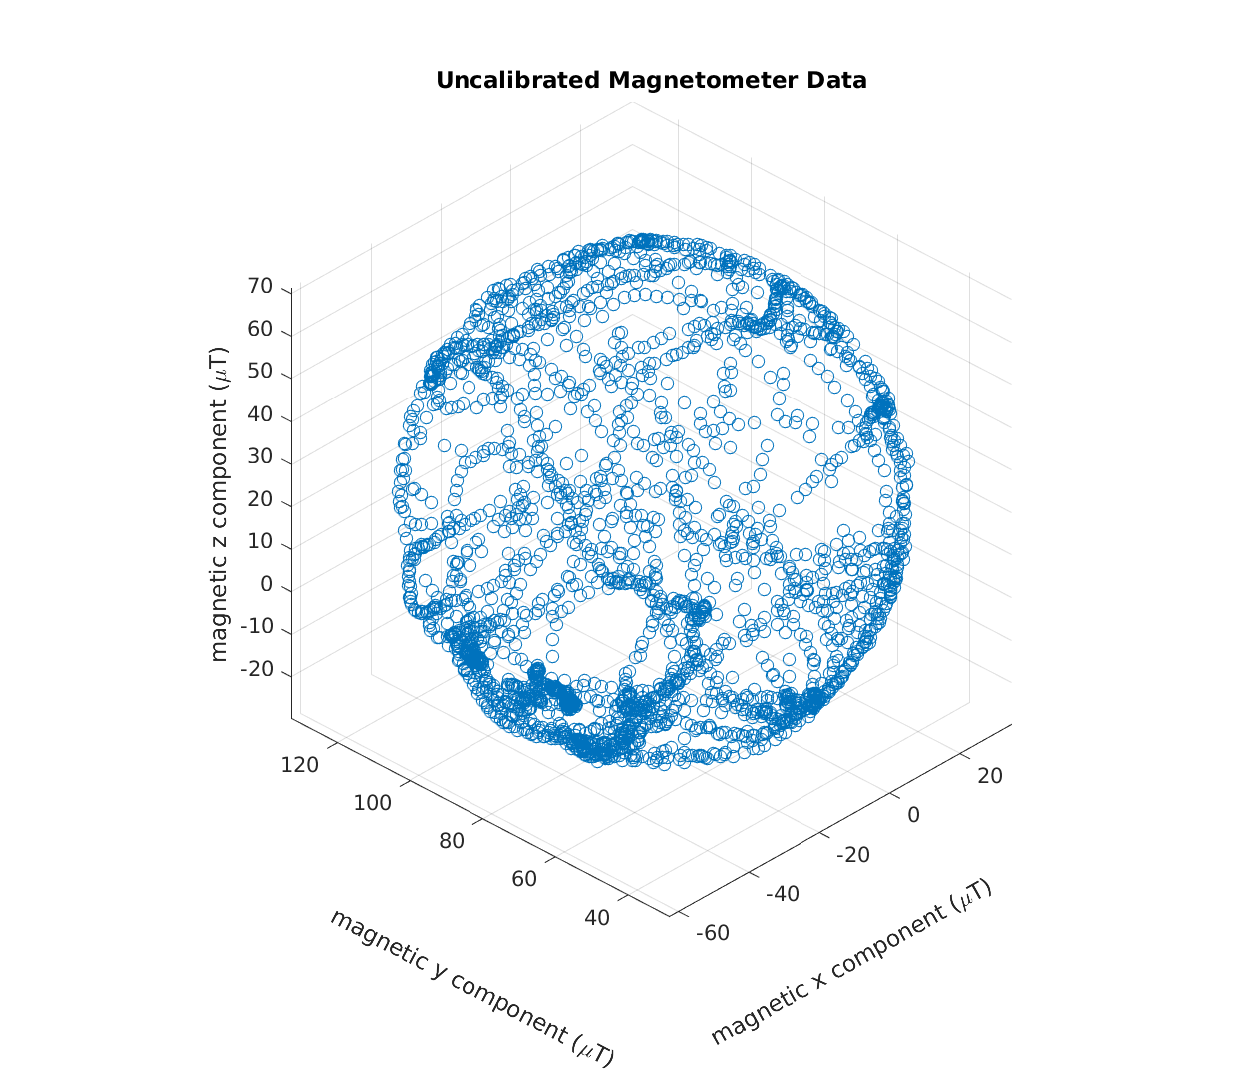
\includegraphics[width=\linewidth]{images/20201020_1125_Uncalibrated_Magnetometer_Data}
		\caption{Uncalibrated magnetometer data}
		\label{fig:uncalibrated_magnetometer_data}
	\end{subfigure}
	\begin{subfigure}[t]{0.4\textwidth}
		\centering
		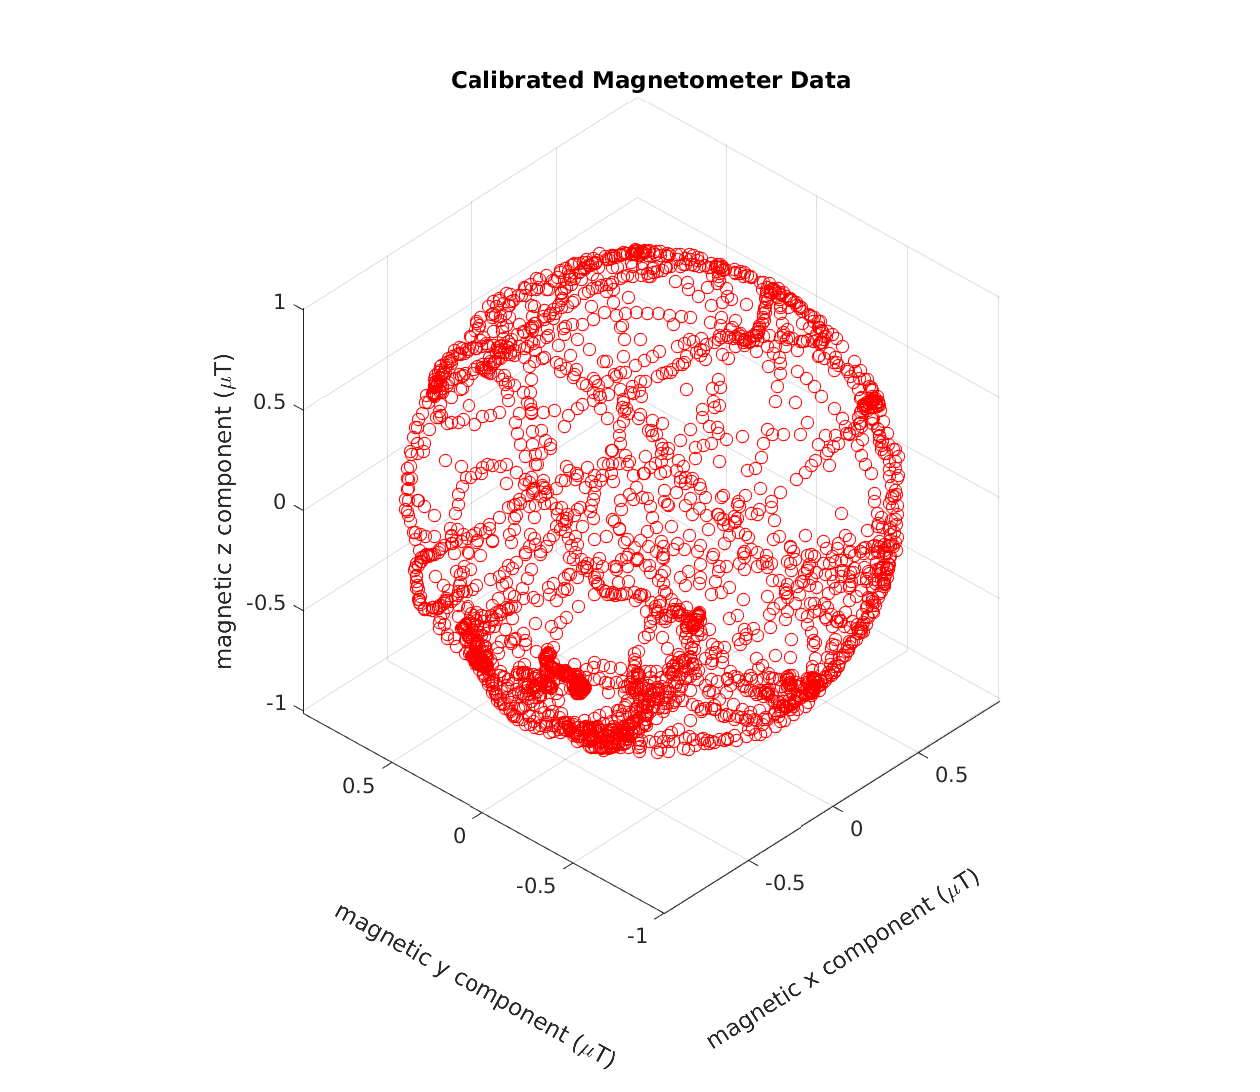
\includegraphics[width=\linewidth]{images/20201020_1125_Calibrated_Magnetometer_Data}
		\caption{ Calibrated magnetometer data}
		\label{fig:calibrated_magnetometer_data}
	\end{subfigure}
	\caption{Magnetometer calibration for smart MEMS IMU in one location}
	\label{fig:calibration_magnetometer}
\end{figure}

\newpage
\subsection{Extended Kalman Filter}
\label{sec:method-EKF}
The Kalman Filter (KF) uses a linear state space model in combination with measurements and its characteristics to make an unbiased minimum-variance estimator \cite{verhaegen2007filtering}. The KF assumes that the noise affecting the state space model is additive and that both process and measurement noise are Gaussian and zero mean.
The Kalman Filter consists of three steps, with the last two steps performed recursively. The first is stating an initial estimate and the variance of the process and measurement noise.  The second is the time update in which the state is propagated through a motion model, which may or may not have an external input, resulting in a one step ahead estimate. The third step is the measurement update in which the estimate generated by the time update is compared with actual measurements related to the state being estimated. Discrepancies between the two will lead to an error measurement. This error can then be used to correct the estimate.
The Extended Kalman Filter (EKF) is an adaptation of the Kalman Filter that estimates for non linear models. 

For orientation estimation the motion and measurement model presented in \eqref{eq:orient_state_space} can be used. As stated in \cref{sec:motion_and_measurement_models}, this model has assumptions that need to be accommodated. This will have to be incorporated in the EKF. Additionally sensor data does not all arrive at the same time. This means that the measurement update will potentially need to only update with either magnetometer or accelerometer data.  

\subsubsection{Time Update}

A time update occurs every time a gyroscope measurement ($y_\omega$) is received. It calculates a one step ahead estimate of the state vector and its covariance matrix. The calculations are as followed: 

\begin{subequations}
\begin{align}
\hat{q}_{t | t-1}^{\mathrm{nb}}=\hat{q}_{t-1 | t-1}^{\mathrm{nb}} \odot \exp _{\mathrm{q}}\left(\frac{T}{2} y_{\omega, t-1}\right) \\
P_{t | t-1}=F_{t-1} P_{t-1 | t-1} F_{t-1}^{\top}+G_{t-1} Q G_{t-1}^{\top}
\end{align}
with $Q = \Sigma_\omega$ and $P$ the state covariance. Here
\begin{align}
F_{t-1}&=\left(\exp _{q}\left(\frac{T}{2} y_{\omega, t-1}\right)\right)^{R},\\
G_{t-1}&=-\frac{T}{2}\left(\hat{q}_{t-1 | t-1}^{\mathrm{nb}}\right)^{L} \frac{\partial \exp _{q}\left(e_{\omega, t-1}\right)}{\partial e_{\omega, t-1}},
\end{align}
\end{subequations}
where $q^L$ and $q^R$ are defined as 
\begin{subequations}
\begin{equation}
q^L = \left(\begin{array}{cc}{q_{0}} & {-q_{v}^{\top}} \\ {q_{v}} & {q_{0} \mathcal{I}_{3}+\left[q_{v} \times\right]}\end{array}\right),
\end{equation}	
\begin{equation}
q^R = \left(\begin{array}{cc}{q_{0}} & {q_{v}^{\top}} \\ {-q_{v}} & {q_{0} \mathcal{I}_{3}+\left[q_{v} \times\right]}\end{array}\right).
\end{equation}
\end{subequations}

\subsubsection{Measurement Update}

A measurement update occurs every time either an accelerometer or magnetometer reading is received. \\
To ensure that the assumptions of the gravity vector being dominant in the accelerometer and the homogeneous magnetic field being dominant in the magnetometer, thresholds can be used. This is of importance with pedestrian dead reckoning, as a walking motion will induce additional external forces, affecting the acceleration measured by the IMU. Additionally, when localizing indoors, magnetic disturbance within the built environment will affect the magnetometer readings.\\
The measurement update for the EKF with quaternions as states is as followed:

\begin{subequations}
	\begin{align}
	\tilde{q}_{t | t}^{\mathrm{nb}} &=\hat{q}_{t | t-1}^{\mathrm{nb}}+K_{t} \varepsilon_{t}, \\
	\tilde{P}_{t | t} &=P_{t | t-1}-K_{t} S_{t} K_{t}^{\top}
	\end{align},
	with	
	\begin{align}
	\varepsilon_{t} &= y_{t}-\hat{y}_{t | t-1},\\
	\quad S_{t} &= H_{t} P_{t | t-1} H_{t}^{\top}+R, \\
	\quad K_{t} &= P_{t | t-1} H_{t}^{\top} S_{t}^{-1}.
	\end{align}
\label{eq:quat_meas_update}	
\end{subequations}


If an accelerometer measurement is received and whos magnitude falls in an interval around the magnitude , the variables to use in \eqref{eq:quat_meas_update} are

\begin{subequations}
	\begin{align}
	y_{t}&=
	y_{\mathrm{a}, t}, \\
	\hat{y}_{t | t-1}&=
	-\hat{R}_{t | t-1}^{\mathrm{bn}} g^{\mathrm{n}},\\
	H_{t}&=	-\left.\frac{\partial R_{t | t-1}^{\mathrm{bn}}}{\partial q_{t | t-1}^{\mathrm{nb}}}\right|_{{q_{t | t-1}^{\mathrm{nb}}}=\hat{q}_{t | t-1}^{\mathrm{nb}}} \quad g^{\mathrm{n}}.
	\end{align}
\end{subequations}

Likewise if a magnetometer measurement arrives and meets the threshold requirement, the variables are defined as

\begin{subequations}
	\begin{align}
	y_{t}&=	y_{\mathrm{m}, t},\\
	\hat{y}_{t | t-1}&=	\hat{R}_{t | t-1}^{\mathrm{bn}} m^{\mathrm{n}},\\
	H_{t}&=	\left.\frac{\partial R_{t | t-1}^{\mathrm{bn}}}{\partial q_{t | t-1}^{\mathrm{nb}}}\right|_{{q_{t | t-1}^{\mathrm{nb}}}=\hat{q}_{t | t-1}^{\mathrm{nb}}} \quad m^{\mathrm{n}}.
	\end{align}
\end{subequations}

\subsubsection{Renormalization}
Once a measurement update occurs the resulting quaternion is not necessarily a unit quaternion, which is a requirement for orientation parametrization. To facilitate this a renormalize the quaternion is required, using

	\begin{equation}
	\hat{q}_{t | t}^{\mathrm{nb}}=\frac{\tilde{q}_{t-1}^{\mathrm{nb}}}{\left\|\tilde{q}_{t | t}^{\mathrm{nb}}\right\|_{2}}.
	\end{equation}

Using steps outlined in \cite{Kok2017} and \cite{Linkoping2013}, the above outlined EKF was implemented in MATLAB. It was preliminarily  tested in a limited case with actual smartphone sensors. Calibration and testing occurred in the same room, where the phone was continuously randomly orientated while recording sensor data. This data was afterwards exported and entered into the EKF. The results can be seen in \cref{fig:simple_stationary_ekf}, where it is compared with the orientation estimation calculated by the android system. It is clear that the orientation estimation is almost identical to the system derived orientation.

\begin{figure}[H]
	\centering
	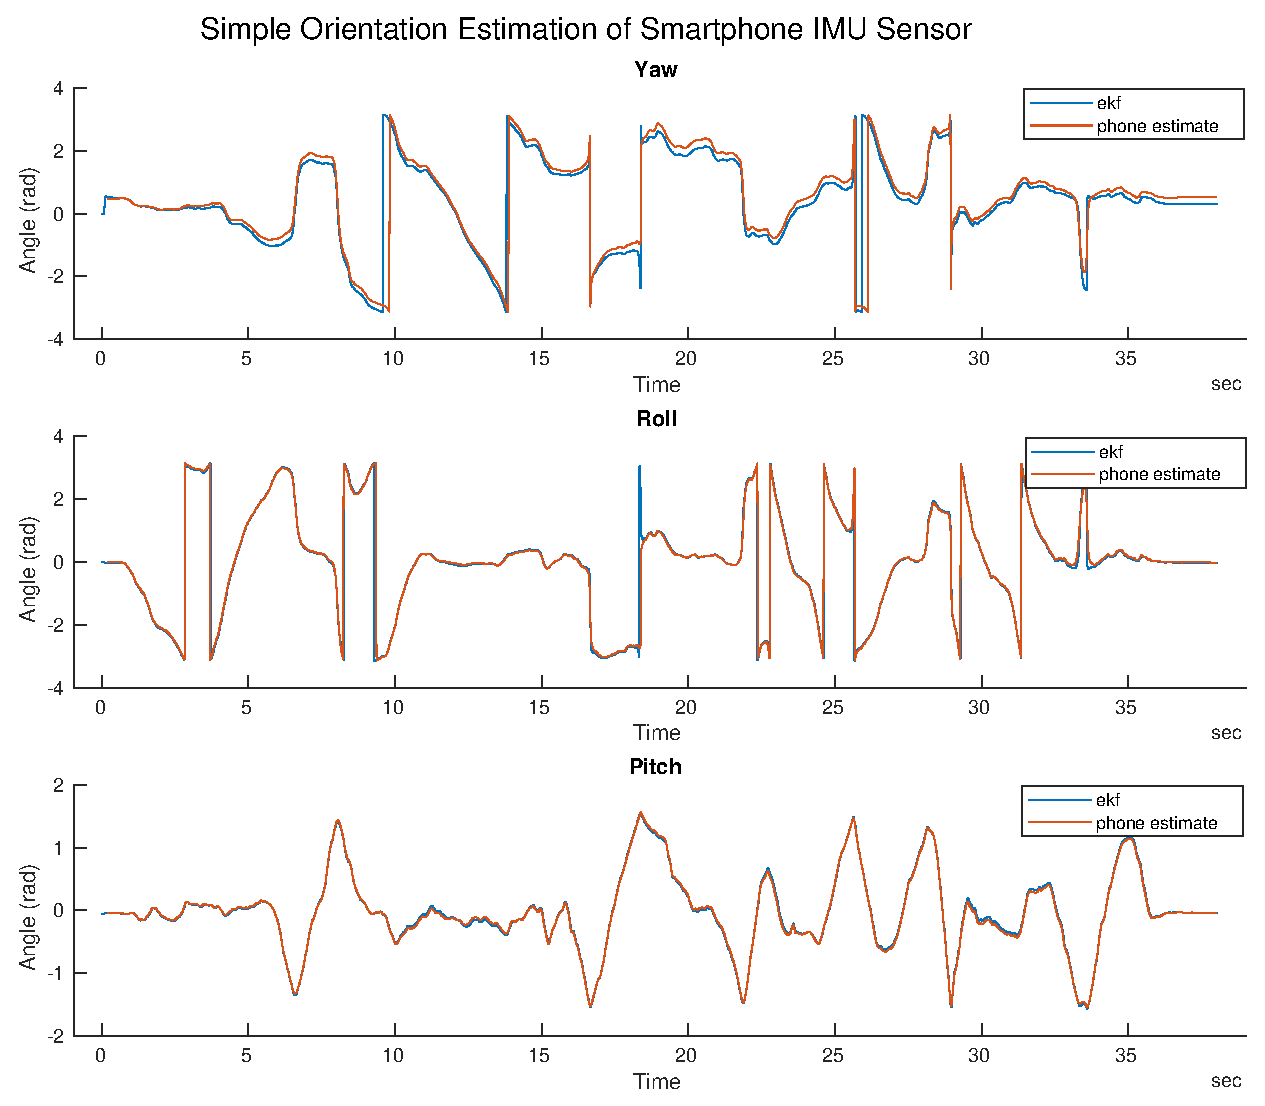
\includegraphics[width=0.7\linewidth]{images/20201025_2015_simple_stationary_ekf}
	\caption[Simple orientation estimation comparison]{ Simple orientation estimation comparison between own EKF and android orientation estimation}
	\label{fig:simple_stationary_ekf}
\end{figure}

\textcolor{red}{what other metrics are important to show to proof the performance of the EKF?}

\newpage
\section{Map based Particle Filter with Landmark Measurement Update}
In \cref{sec:rw-drift_reduction}, the Particle Filter was introduced as a drift reduction method able to handle spatial context such as map information, landmarks and spatial models. In this section, the spatial information of the experimental setup is shown and the implementation of the particle filter with step and heading system input is presented.

\subsection*{Map Creation}
In order to use spatial context with the particle filter, different sources were combined to generate a map of the experiment space. Rudimentary blueprints of the building were used generate a diagram of the indoor environment. The positioning and size of furniture was estimated. The resulting image has clear color distinction between the different structures within the building, including walls, doors and furniture, as seen in \cref{fig:indoor_blueprint}. Through a comparison between structures in the generated image and satellite images, shown in \cref{fig:house_google_maps}, the image was transformed from pixel to meter coordinates. This provides the basis for incorporating spatial context within a Particle Filter.

\begin{figure}[H]
	\centering
	\begin{subfigure}[t]{.38\textwidth}
		\centering
		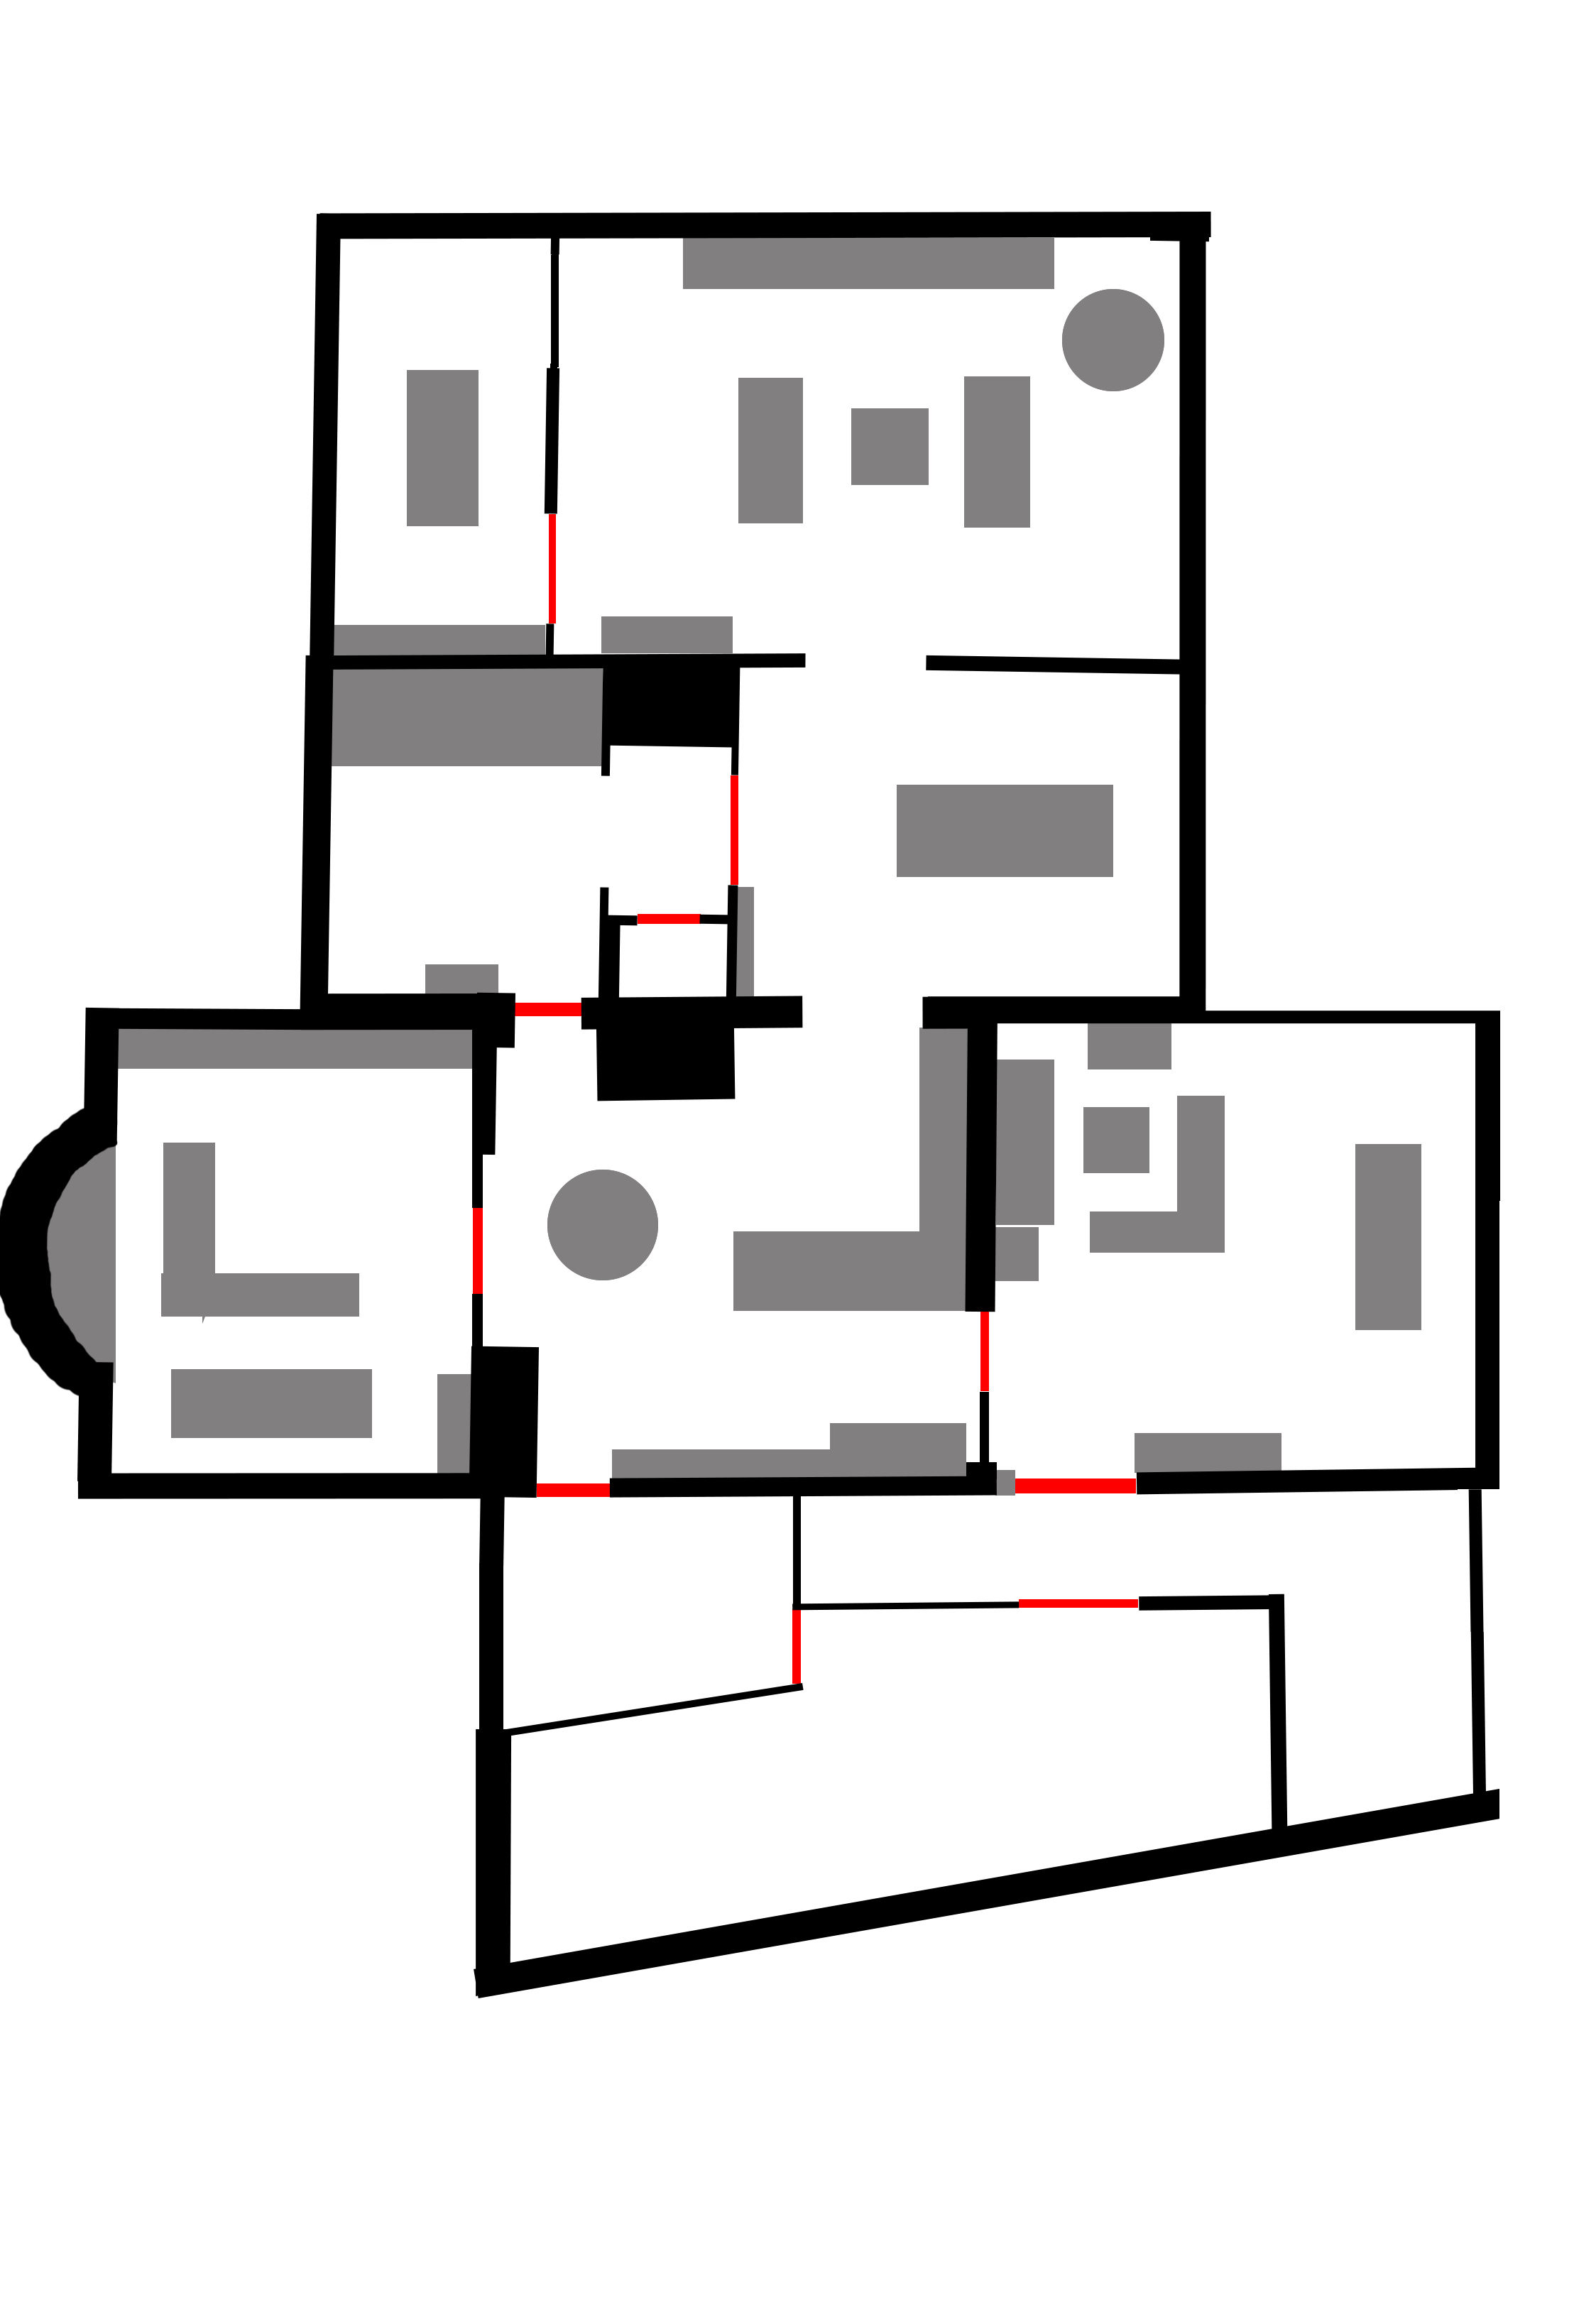
\includegraphics[width=0.9\linewidth]{images/indoor_blueprint}
		\caption[Image from building blueprints]{Image from building blueprints. Black, grey and red represent walls, furniture, and doors, respectively.}
		\label{fig:indoor_blueprint}
	\end{subfigure} \quad
	\begin{subfigure}[t]{.4\textwidth}
		\centering
		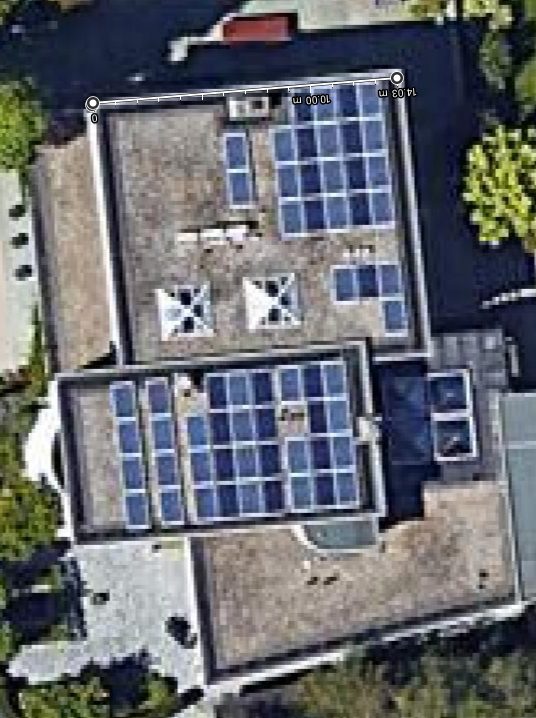
\includegraphics[width=0.9\linewidth]{images/house_google_maps}
		\caption{Measurement from Google Maps}
		\label{fig:house_google_maps}
	\end{subfigure} \quad
	\label{fig:particle_map_construction}
	\caption{Particle filter map creation}
\end{figure}

\subsection*{Implementation}

The implementation of the particle filter for indoor localization using SHS trajectory and activity recognition as input will be explained next.  \cref{algo:bootstrap_PF} summarizes the whole approach.

\subsubsection*{Initialization}
For indoor localization on one floor, particles are limited to $\mathbb{R}^{2}$ and by the outer perimeter of the building the user is located in. The particle is defined by 

\begin{equation}
x_k^i = \left(\begin{array}{l}
p_{1,k}^i   \\
p_{2,k}^i  \\
\theta_k^i
\end{array}\right), 
\label{eq:pf_state}
\end{equation}
where $x^i_k$ is the state of particle $i$ at time $k$, $p_1 $ and $p_2$ are the particle x axis and y axis position respectively. The heading angle is  $\theta$.\\
For initialization,  all particles are positioned around a known starting point. The initial weight of each particle $\omega^i$ is $1/N$, where $N$ is the total number of particles. Once initialized the following three steps are performed recursively \cite{Wu2019,Woodman2008}: 

\begin{enumerate}
	\item \textbf{Measurement update} \\
	There are two measurement updates possible within the particle filter, one that compares particle trajectories to map constraints and the other were door positions are compared with particle positions. \par 
	
   With a map, the position of physical structures can be compared with the trajectory of particles as a measurement update. If these structures cannot be traversed, as is the case with walls, the trajectory of a particle that crosses such a structure is incorrect. This makes the likelihood of it being a position estimate 0, rendering its weight 0 as well. Particles that traverse accessible regions have a likelihood of 1, and therefore also a weight of 1. This form of measurement turns wall information into a two dimensional probability density function ($p_{\scaleto{map}{4pt}}$). A grid based spatial model was used in which each pixel that contained some form of obstruction was label as inaccessible for particles in the particle filter. The result is shown in \cref{fig:pf_map}, where black color regions are inaccessible and have a likelihood of 0.\\
   Depending on this distribution, the individual particle weights are evaluated as 
   
   \begin{subequations}
   	\begin{equation}
   		\omega^i_{k|k} = \frac{1}{c_k} \omega^i_{k|k-1} p_{\scaleto{map}{4pt}}(x^i_{k:k-1}),
   		\label{eq:pf_map_weight}	
   	\end{equation}
   	\begin{equation}
   		c_{k}=\sum_{i=1}^{N} w_{k | k-1}^{i} p_{\scaleto{map}{4pt}}\left( x^i_{k:k-1}\right).
   		\label{eq:pf_map_normalization}
   	\end{equation}
   	\label{pf_map_update}
   \end{subequations}
   
   Here $x^i_{k:k-1}$ represent the indivifual particle path between its current and previous particle positions. This measurement update occurs every timestep of the step and heading system.
   
   
   
   	\begin{figure}
   	\centering
   	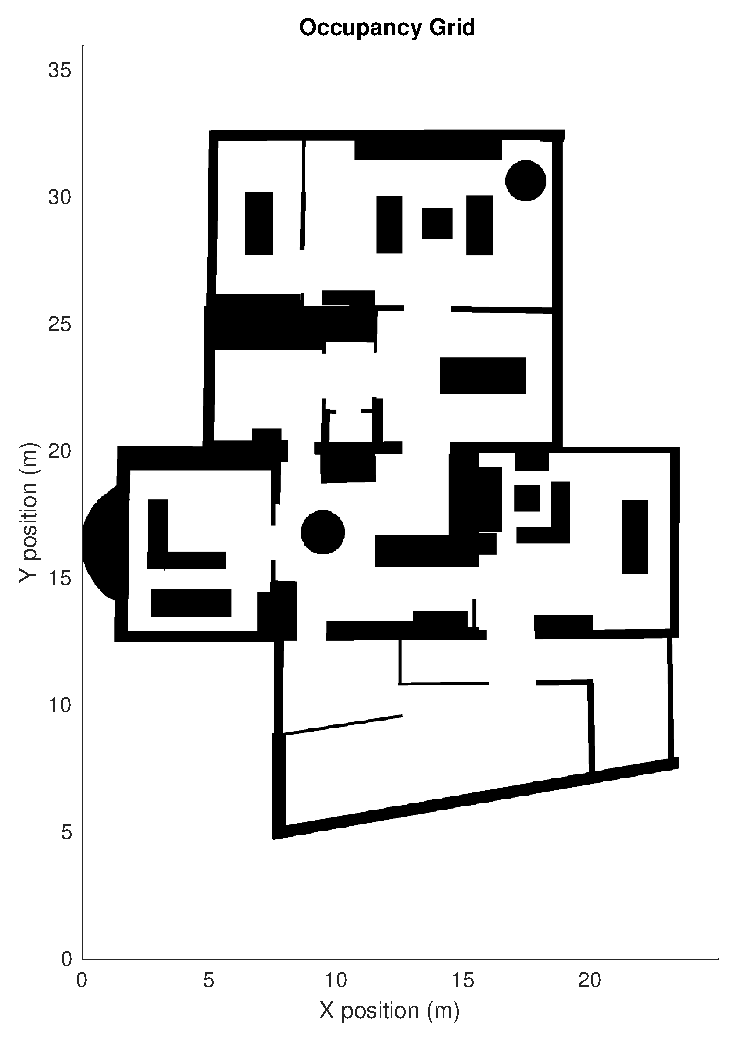
\includegraphics[width=0.4\linewidth]{images/20201030_1157_pf_map_1}
   	\caption{Particle Filter two dimensional probability function, where white and black has a probability of 1 and zero, respectively.}
   	\label{fig:pf_map}
   \end{figure}
   
	A map also indicates door locations, which are used as landmarks. If a door opening is detected through activity recognition, a conditional probability at each particle can be used to determine its weight, as 
	\begin{subequations}
		\begin{equation}
			c^*_{k}=\sum_{i=1}^{N} w_{k | k}^{i} p_{\scaleto{door}{4pt}}\left(y_{k} | x_{k}^{i}\right)
			\label{eq:pf_door_normalization}
		\end{equation}
		\begin{equation}
			\omega^{i*}_{k|k} = \frac{1}{c^*_k} \omega^i_{k|k} p_{\scaleto{door}{4pt}}(y_k|x^i_k),
			\label{eq:pf_door_weight}	
		\end{equation}
	\end{subequations}

 In the case of \cref{fig:pfdiagram}, if a door activity is detected the weight of particles P1 and P3 will be made higher than that of P2. This measurement update can only happen when a door interaction detection occurs, and happens after the map constraint measurement update.
	
	\begin{figure}[]
			\centering
			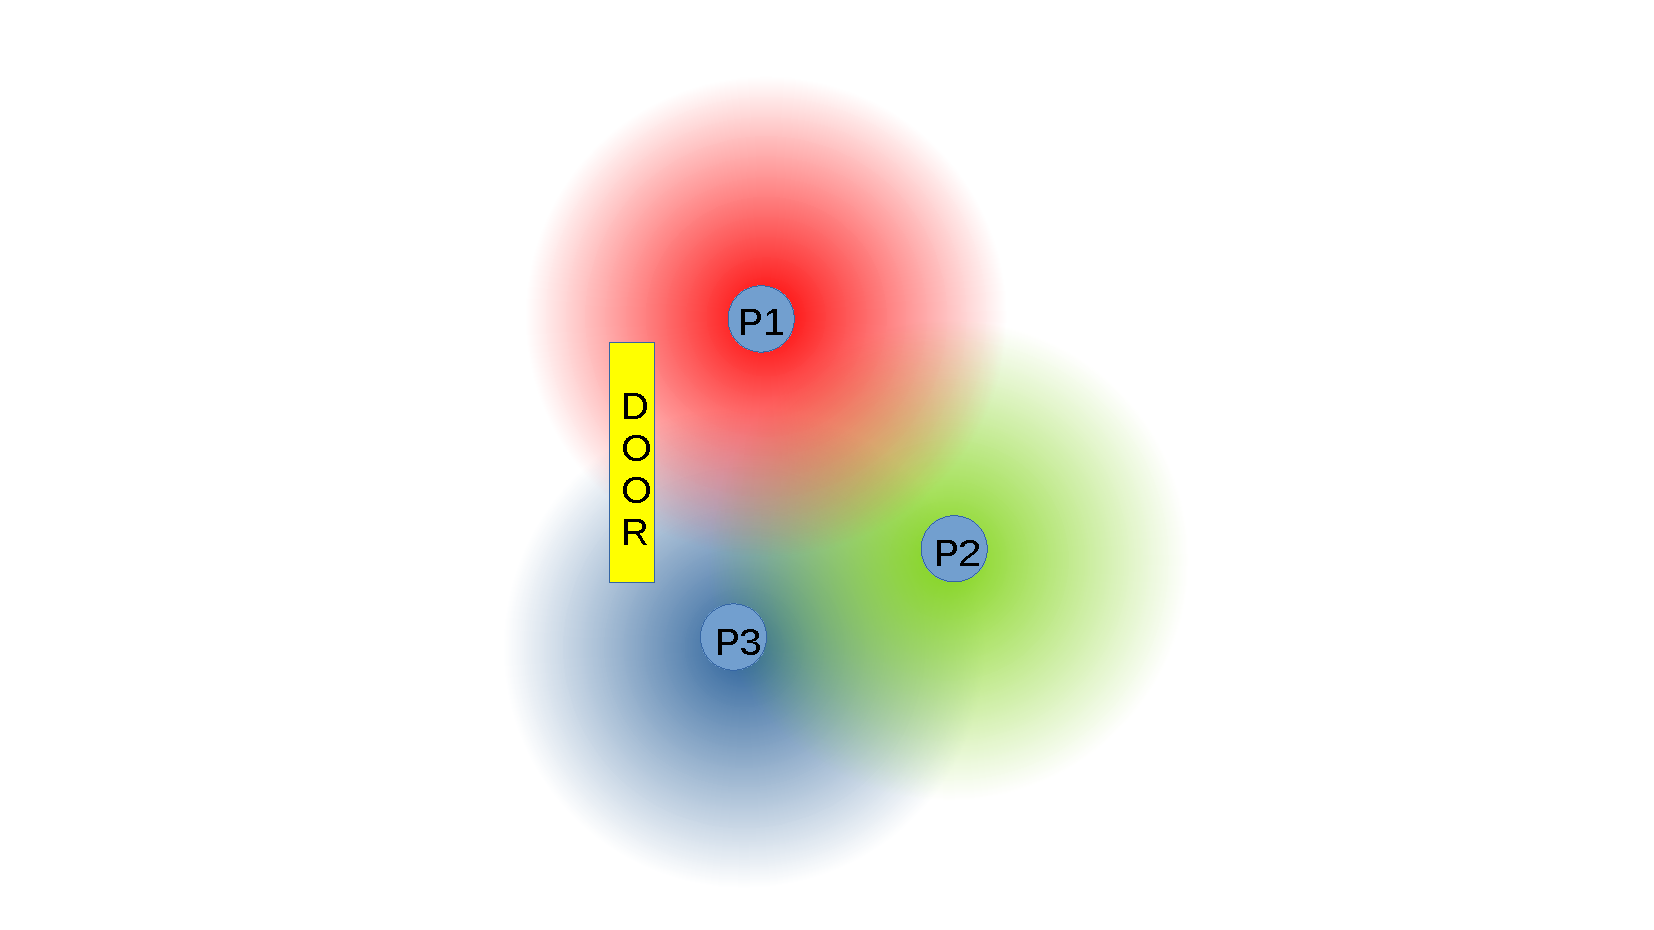
\includegraphics[trim=240 0 220 0, clip, width=0.35\linewidth]{images/pf_diagram}
			\caption{ Particles with a multivariate normal probability density function, represented by color gradient. At door interaction detection, particle weight is determined by probability at location of door in individual density functions.}
			\label{fig:pfdiagram}
	\end{figure}
	
	\item \textbf{Resampling}\\
	Resampling is used to select a new group of particles based on the weights of the current particles. The higher the weight of a particle is, the more likely it will be resampled. A particle can even be resampled multiple times. \par 
	There are multiple methods that can be used for resampling including multinomial, stratified, systematic, and	residual resampling \cite{hol2006resampling,gustafsson2010statistical}. \citet{hol2006resampling} conclude that  systematic resampling is the best considering resampling quality and computational complexity. Systematic resampling is defined as 
	
	\begin{align}
		x^{i*} &= x(F^{-1}(u^i)) \\
		u^i &= \frac{(i-1) + \tilde{u}}{N}, \tilde{u} \sim \mathcal{U}[0,1).
	\end{align}	
	
	 Here $x^{i*}$ represents the newly sample particle with index $i$, $F^{-1}$ represents the generalized inverse of the cumulative probability distribution of the normalized particle weights. Once the particles are resampled the particle weights are reset with $\omega^i_{k+1|k} = 1/N$ . \par
	Resampling inevitably destroys information and therefore increases uncertainty by the random sampling \cite{gustafsson2010particle}. Resampling should therefore occur only when it is needed. \citet{gustafsson2010statistical} proposes the use of  \textit{effective number of samples} to trigger a  resampling. This can be calculated as 
	\begin{subequations}
		\begin{equation}
		N_{\mathrm{eff}}=\frac{1}{\sum_{i=1}^{N}\left(w^{i}\right)^{2}},
		\end{equation}
		
		where
		
		\begin{equation}
		1 \leq N_{\mathrm{cff}} \leq N.
		\end{equation}
	\end{subequations}
	
	The resampling condition can then be defined as $N_{eff} < N_{th}$ \cite{gustafsson2010statistical}, where the threshold can be placed at $N_{th} = 2N/3$, with $N$ being the total number of particles.
	
	
	\item \textbf{Time update} \\	
	After resampling, the new particles update their state with a dynamic model. For indoor localization using a step and heading trajectory as input, the dynamic model used is
	
	\begin{equation}
		\label{eq:SHS_dynamic_model_with_noise}
		x^i_{k + 1}
		=
		\left(\begin{array}{l}
			p_{1,k}^i + (l_{k} + e_l) * \cos (\theta_{k}^i) \\
			p_{2,k}^i + (l_{t} + e_l) * \sin (\theta_{k}^i) \\
			\theta_{k}^i + \Delta \phi + e_\theta 
		\end{array}\right), \quad
		e_{\theta} \sim \mathcal{N}\left(0, \sigma_{\theta}^{2}\right), \quad e_{l} \sim \mathcal{N}\left(0, \sigma_{l}^{2}\right).
	\end{equation}

The inputs to this dynamic model are $l_{t}$, which is the step length found by step detection and step length estimation, and $\Delta \theta_t$, which is the change in heading between the current and previous timestep of the step and heading trajectory, found through the orientation estimation. These variables have additive zero mean Gaussian noise realizations $e_{\theta}$ and $e_{l}$, representing the uncertainty in the values of these inputs.
\end{enumerate}
The resulting particle filter from the previous steps is summarized in \cref{algo:bootstrap_PF}.

\begin{algorithm}[H]
	\small
	\SetAlgoLined
	\caption{Indoor Localization Particle Filter}
	\label{algo:bootstrap_PF}
	$i = 1,...,N$.   \\
	% choose a proposal distribution $ q(x_{k+1}|x_{1:k},y_{k+1})$, resampling strategy and the number of particles N.\\
	% \KwResult{Write here the result }
	\underline{Initialization:}\\
	choose the number of particles N.
	Generate initial distribution with
	\begin{subequations}
		\begin{equation}
			x^i_1 \sim p_{x_1},
		\end{equation}
		and let
		\begin{equation}
			\omega^i_{1|0} = 1/N.
		\end{equation}
	\end{subequations}
	
	\For{k = 1,2,...}{
		\underline{Measurement update:}\\
		\begin{subequations}
			\begin{align}
				\omega^i_{k|k} &= \frac{1}{c_k} \omega^i_{k|k-1} p_{\scaleto{map}{4pt}}(x^i_{k:k-1}),
				\label{eq:algo_pf_map_weight}\\	
				c_{k} &=\sum_{i=1}^{N} w_{k | k-1}^{i} p_{\scaleto{map}{4pt}}\left( x^i_{k:k-1}\right)
				\label{eq:algo_pf_map_normalization}
			\end{align}
			\label{pf_map_update}
		\end{subequations}
		
		
		\begin{subequations}
			
			\If{(door interaction detected)}{
				\begin{align}
					c_{k}&=\sum_{i=1}^{N} w_{k | k}^{i} p_{\scaleto{door}{4pt}}\left(y_{k} | x_{k}^{i}\right)
					\label{eq:pf_door_normalization} \\			
					\omega^i_{k|k} &= \frac{1}{c_k} \omega^i_{k|k} p_{\scaleto{door}{4pt}}(y_k|x^i_k),
					\label{eq:pf_door_weight}	
				\end{align}
			}
			\label{eq:pf_door_update}			
		\end{subequations}\smallskip
		
		
		\underline{Resampling:}\\
		\begin{subequations}
			\begin{equation}
				N_{\mathrm{eff}}=\frac{1}{\sum_{i=1}^{N}\left(w^{i}\right)^{2}},
			\end{equation}
			\If{	$N_{\mathrm{eff}} < 2N/3$}{
				
				\begin{align}
					x^{i*} &= x(F^{-1}(u^i)) \\
					u^i &= \frac{(i-1) + \tilde{u}}{N}, \tilde{u} \sim \mathcal{U}[0,1).\\
					\omega^i_{k+1|k} &= 1/N
				\end{align}
				
				\label{eq:pf_resampling}	
		}	\end{subequations}\smallskip
		\underline{Time update:}\\
		\begin{equation}
			\label{eq:algo_SHS_dynamic_model_with_noise}
			x^i_{k + 1}
			=
			\left(\begin{array}{l}
				p_{1,k}^i + (l_{k} + e_l) * \cos (\theta_{k}^i) \\
				p_{2,k}^i + (l_{t} + e_l) * \sin (\theta_{k}^i) \\
				\theta_{k}^i + \Delta \phi + e_\theta 
			\end{array}\right), \quad
			e_{\theta} \sim \mathcal{N}\left(0, \sigma_{\theta}^{2}\right), \quad e_{l} \sim \mathcal{N}\left(0, \sigma_{l}^{2}\right).
		\end{equation}		
	}
\end{algorithm}
\newpage

\textbf{State Estimation}\\
The Particle Filter is able to estimate non linear posterior densities, allowing for multimodal distributions \cite{gustafsson2010particle,kihlberg2012map}. Multimodal distribution refers to distributions with multiple maxima in the probability density function. This allows the particle filter to have multiple hypotheses for the system that it is modeling. In the case of localization, this translates to indicating that there are two position estimates that are equally as likely based on the information that the filter has received so far. This can occur due to symmetry in the indoor environment \cite{Woodman2008}.

The posterior distribution is the primary output of a particle filter \cite{gustafsson2010particle}. For state inference purposes a single point estimate is more convenient \cite{Saha2009}. The weights and positions of the particle cloud can be used to generate a single point estimate \cite{gustafsson2010particle}. There are different ways of defining the eventual position estimate. The maximum a posteriori (MAP) estimate picks the particle with the highest weight from the posterior distribution \cite{Saha2009}, while the  minimum mean square error (MMSE) estimate calculates a weighted mean \cite{gustafsson2010particle,Saha2009}.\par 

For the particle filter method outlined in this thesis, both forms have disadvantages.
Firstly, MMSE does not work well in situations in which there are multiple equal likely hypotheses \cite{Saha2009}. In such a case it will take the position in between the different hypothesis as the position estimate. A good example of this can be found in \cref{fig:lopen_11_mmse_estimator}. The figure shows the output of a particle filter after 10 time steps. There are clear groups visible, all moving in different directions. The position estimate is expected to be in either one of the particle clouds, however RMSE put it between the different clouds, a position in which no particles are found, making it a subpar estimate. \par 
Implementing MAP as the state estimate in the particle filter is actually similar to MMSE. The measurement update that occurs every timestep of the step and heading trajectory is the one that compares particle trajectories to map constraints, setting infeasible particles probability to zero and feasible particles to one. All feasible particles will then have the same weighting. Since all particles have the same weight, a MAP cannot be defined.
\begin{figure}[]
	\centering
	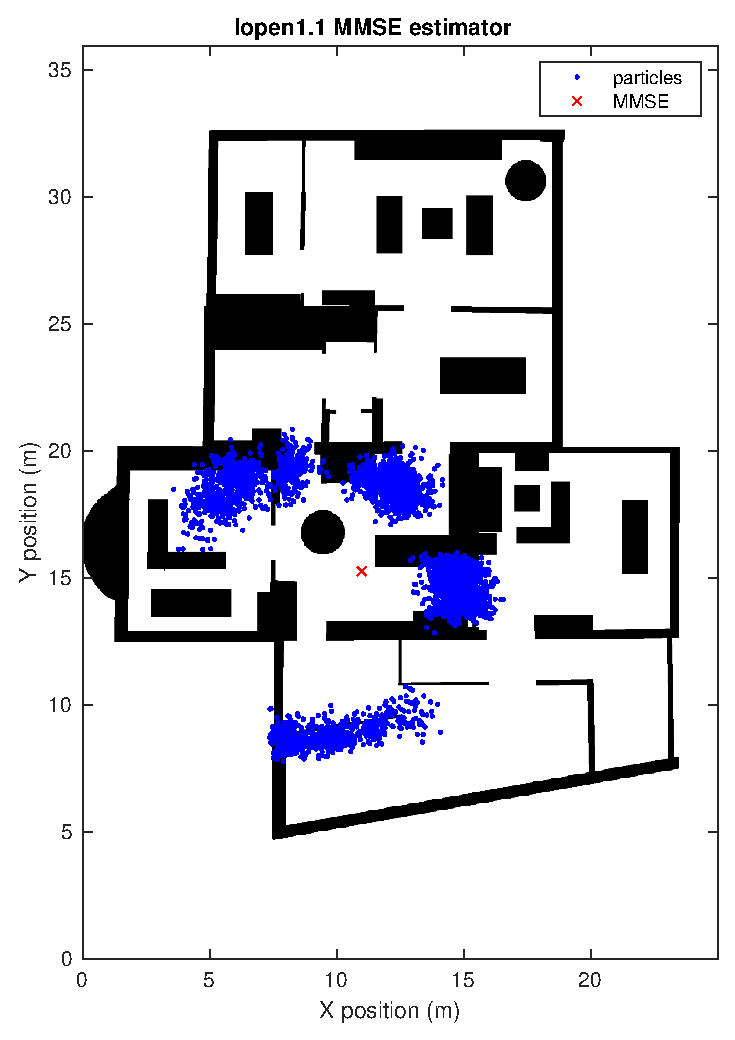
\includegraphics[width=0.35\linewidth]{images/20201108_1751_lopen1_1_MMSE_estimator}
	\setlength{\belowcaptionskip}{-20pt}
	\caption{Particle filter after 10 iterations, showing how MMSE does not provide a suitable single point estimate.}
	\label{fig:lopen_11_mmse_estimator}
\end{figure}

A different approach is to using the particles at the last timestep of the SHS trajectory and calculate all ancestors of these particles. A final particle with all its ancestors generate a feasible trajectory.  Averaging the trajectories of multiple final particles can give an estimate trajectory within the indoor environment.

\section{Activity Recognition}
\label{sec:method-AR}

Activity recognition is large research field in which methods span a broad range of complexity, from simple thresholding to the use of deep learning techniques such as neural networks and its many variations \cite{Lima2019}. Even the subset of activity recognition that use IMU sensors does not decrease the amount of possibilities significantly.

%TODO add drear as activity recognition

The choice for a particular activity recognition method is often a trade-off between performance and computational complexity \cite{Bulling2014}. Considering the scope of this thesis, certain constraints can be applied, such as that the system should be able to function on a smartphone and must use comparable sensors to those found in such devices, thus MEMS IMUs. \citet{Shoaib2015} have performed an extensive survey that focuses on the online activity recognition solely using mobile phone sensors and onboard processing. Other metrics such as resource consumption were also presented. 30 papers were found to meet the requirements of the review. Within the review they indicate that most commonly used classification methods include Decision Tree, support vector machine (SVM), K-nearest neighbor (KNN) and Naive Bayes, in descending order. A third of the papers were found to use decision trees. All but 6 of the papers had the training process occurring offline. The classification process takes the method generated offline, and uses it online to classify new activities. The authors refrain from listing any performance measures, such as accuracy or precision, since no direct comparison between the different methods is made. \citet{Ahmad2020} specifically focuses on seeing whether smartphone activity recognition techniques are also applicable to smartwatches, and what parameters, including classifiers, work best. Activities to recognize included walking, up-stairs, down-stairs, running, and jogging. Their results indicated that  Decision Trees, SVM and KNN had around 90 percent accuracy a minor difference. \citet{Shoaib2016} show that combining information from both a smartwatch and smartphone, complex human activity recognition is improved compared to when only a smart watch is used. 


\textcolor{purple}{ section overview:
\begin{itemize}
	\item Many different type of activity recognition methods, from simple to complex. 
	\item Depends on what needs to be detected. For activities with a clear time based foot print, simple method can be good enough. It is possible to construct own decision tree.
	\item \cref{fig:stand_still_detection_from_shs} shows ground truth first door interaction and the accelerometer traces from a smartwatch and a standstill detection from SHS.
	\item standstill detection from SHS is made by determining when the period buildup between steps exceeds over 3 seconds.
	\item A simple manually constructed decision tree can be used to indicate door interaction. Using both smartwatch data and shs standstill detection the system can distinguish between standing still and interaction with a door.  
\end{itemize}}

\begin{figure}[H]
	\centering
	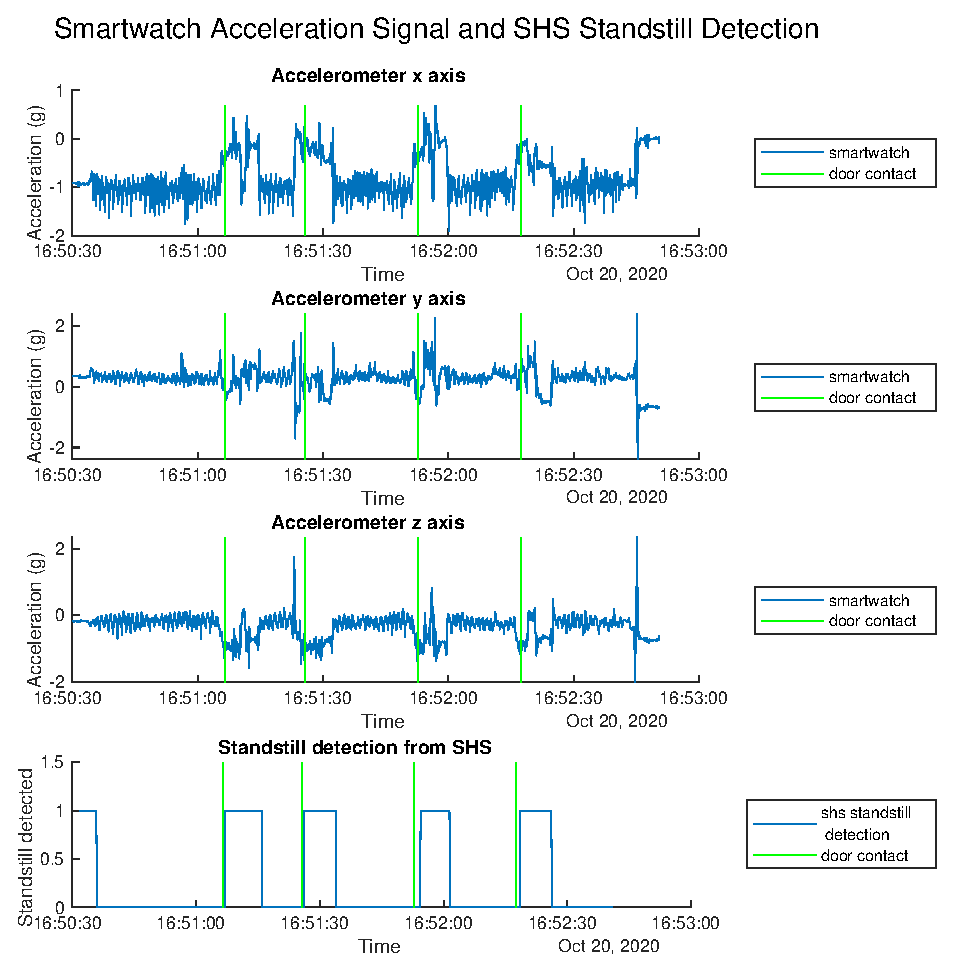
\includegraphics[width=0.7\linewidth]{images/20201103_1325_Standstill_detection_from_SHS}
	\caption{Smartwatch accelerometer data and SHS stand still detection}
	\label{fig:stand_still_detection_from_shs}
\end{figure}

\begin{figure}[H]
	\centering
	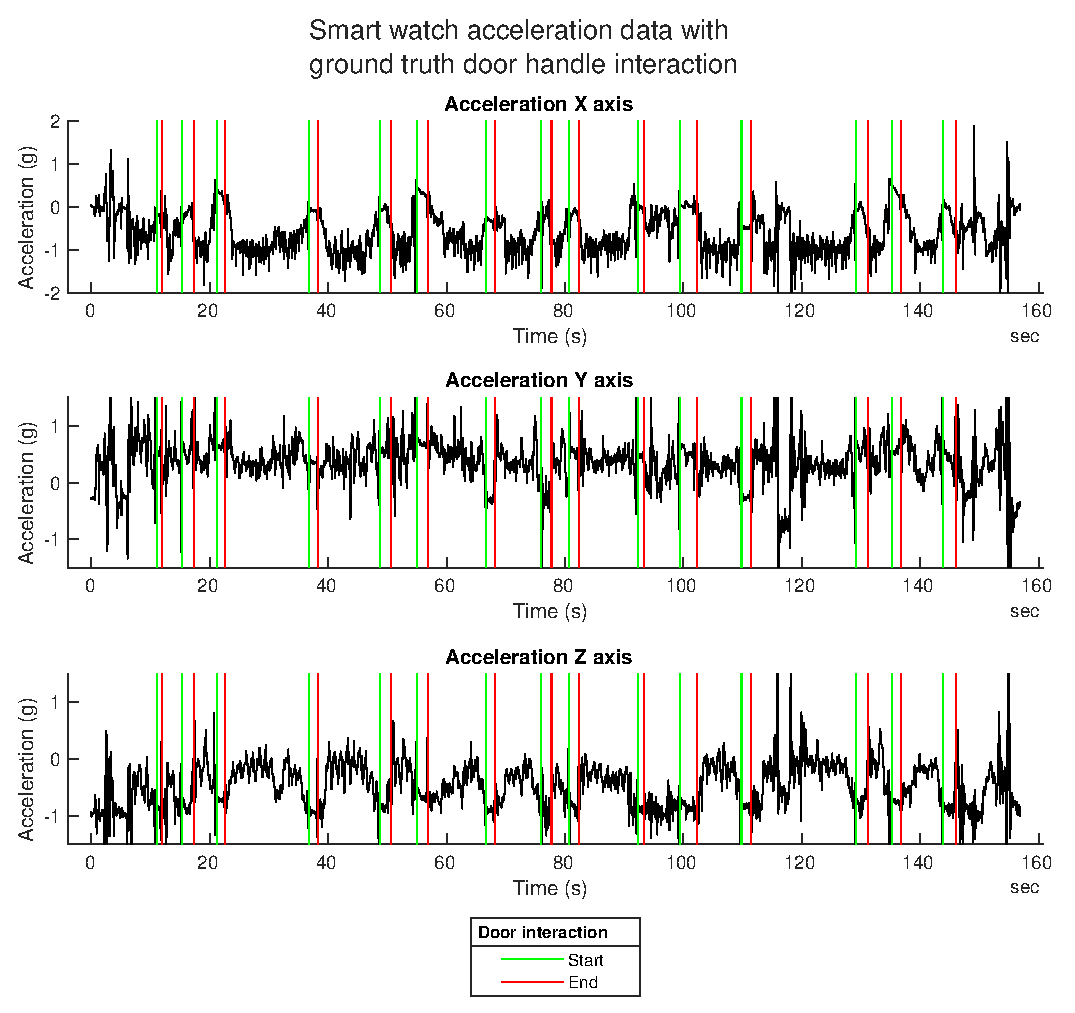
\includegraphics[width=0.7\linewidth]{images/20201114_1820_smartwatch_acc_with_gt_door_and_door_detect_1}
	\caption{}
	\label{fig:202011141820smartwatchaccwithgtdooranddoordetect1}
\end{figure}

\begin{figure}[H]
	\centering
	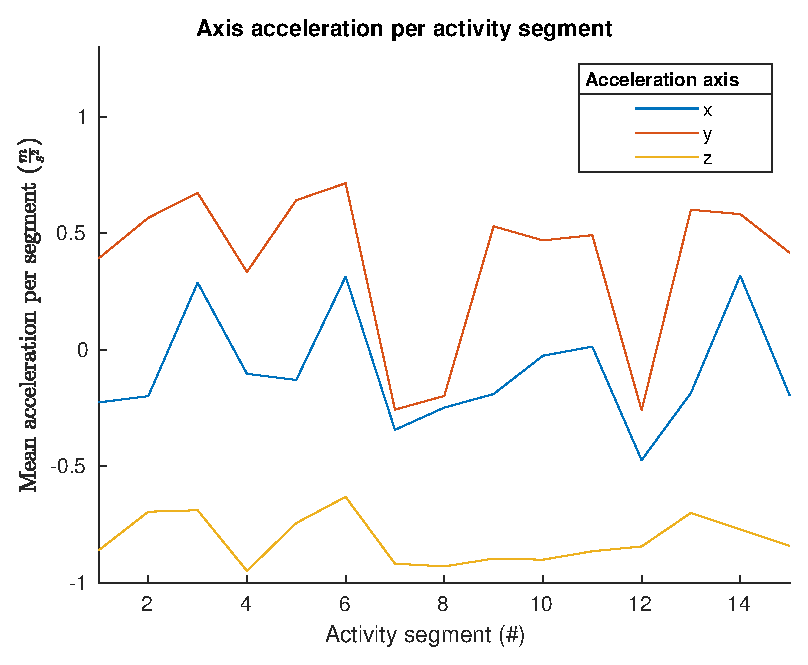
\includegraphics[width=0.7\linewidth]{images/20201114_1858_Axis_acceleration_per_activity_segment}
	\caption{}
	\label{fig:202011141858axisaccelerationperactivitysegment}
\end{figure}

\begin{figure}[H]
	\centering
	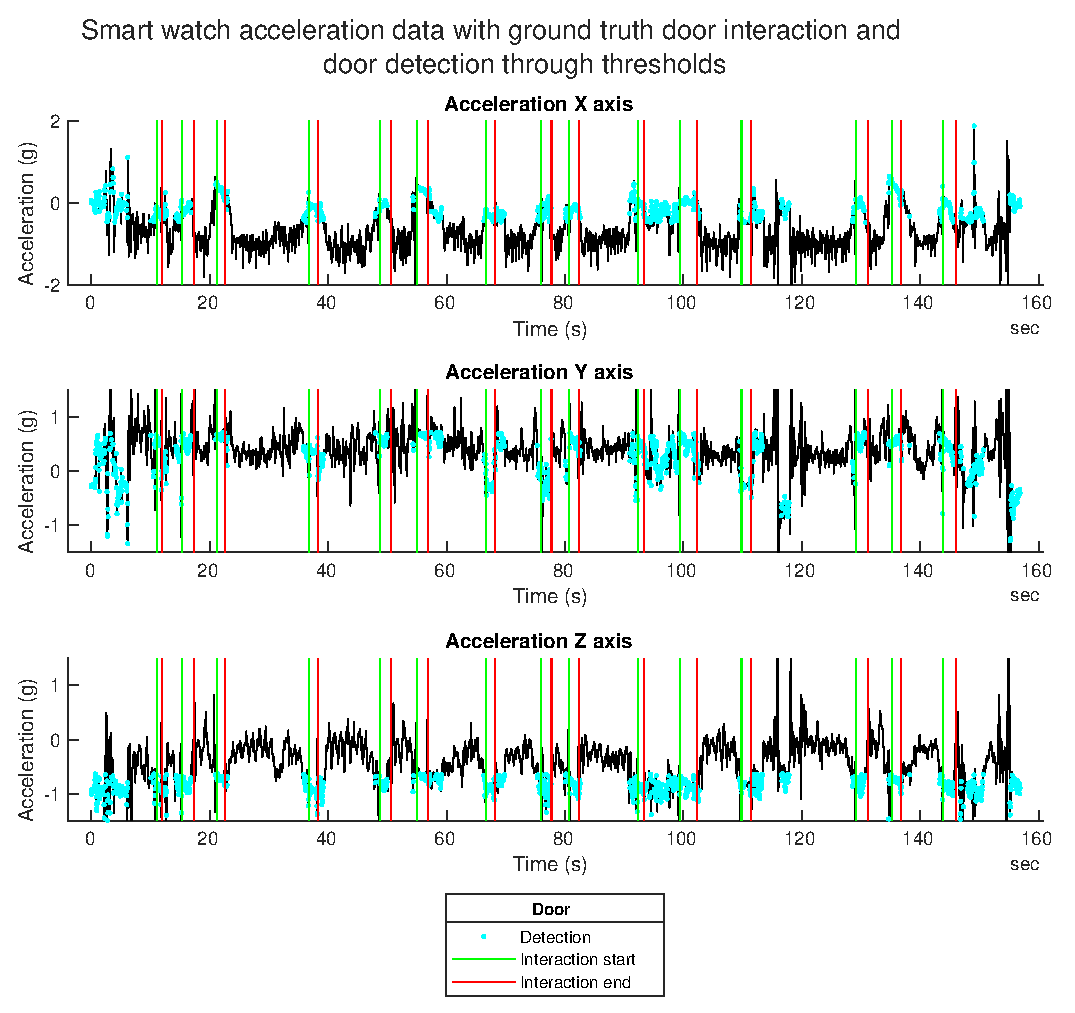
\includegraphics[width=0.7\linewidth]{images/20201114_1820_smartwatch_acc_with_gt_door_and_door_detect_2}
	\caption{}
	\label{fig:202011141820smartwatchaccwithgtdooranddoordetect2}
\end{figure}

\textcolor{red}{I have more data on smartwatch accelerometer also from different people. I can use that data to determine the threshold on accelerometer data that would work on different people. Do you think that this is a good idea?}
\chapter{Experimental Results}

\textit{In this chapter, the  different components of the proof of concept explained in \cref{chap:method}are tested and the results shown. First, the  experimental setups are outlined. Afterwards the \ac{SHS} components outlined in \cref{chap:method} are tested individually. Hereafter the whole SHS-PF with activity recognition is treated.}

\section{Experimental Setups}
\label{sec:results-experimental setup}
In order to determine the performance of the \ac{SHS} \ac{PF} and its components, different experiments were devised. \par 

The step detection and step length estimation components are tested using a combination of data made available online under an open license and original data collected. The online data used for step detection and length estimation derive from the research upon which the individual methods are based on. The advantage of using online data is that it allows testing of techniques using the data from multiple test subjects holding a smartphone in multiple carrying modes, without having to perform extensive experiments.  \par 

The original data was collected personally, using an available smartwatch and smartphone. The step detection and step length estimation experiments for gathering original data  were performed outdoors using only a smartphone carried in the "in front, in hand" carrying mode, as in \cref{fig:experiment_carrying_position}. This was done since the location has no effect on accelerometer readings and outdoor testing allows for long straight walking distances, which are also easily measured from satellite images.\par 

For step detection, accelerometer measurements were recorded using different carrying modes while counting the number of steps. For step length estimation, known distance were walked and compared with the total distance estimated using the devised method. Further details on the experiments can be found in their respective sections, \cref{sec:results-step_detection} and \cref{sec:results-step_length_estimation}.    \par

Since orientation estimation and the whole indoor localization system are location-dependent, experiments were performed indoors. This was located at the residential property introduced in \cref{sec:method-particle_filter}. The tests consisted of walking around indoors with an android smartphone in hand and recording the \ac{IMU} signals in the phone through a dedicated android app. In addition, a smartwatch was worn around the wrist of the hand that was not holding the smartphone. This hand was used to open and close doors. The opening of doors was also indicated manually through the app on the smartphone, which had a button to record timestamps when pressed.\par 

In addition to recording \ac{IMU} data from both smartphone and smartwatch while the path was being walked, the trials were also being filmed from a breast pocket by another device. The video recordings are used to get a rough estimate of the path walked during the trial. This was done by replaying the video and pausing it at one second intervals. At the paused moments, the approximate position was manually indicating on the map of the experiment location. The map position and time elapsed since the start of the trial were recorded. The resulting trajectory can be used to give a rough performance indication of the indoor localization method. The full experimental process can be found in \cref{appendix:shs_experiment}. \par

A total of 6 successful trials were walked by one test subject, each trial trying to generate a different trajectory than the previous trials. The same person that generated the original data for the step detection and step length estimation experiments was also used for the indoor orientation and localization experiments.\par 


\section{Step Detection Performance}
\label{sec:results-step_detection}
The step detection method presented in \cref{sec:meth - step detection} is tested on both online and original data. In this section, first an overview of the relevant online data will be given, followed by several different metrics with which the performance of the step detection method from \cref{sec:meth - step detection} is evaluated. 


\subsection{Online Data}
\citet{Salvi2018} have released the raw accelerometer data used for their step detection algorithm under an open license. The raw data of the validation set consists of sampling time and three raw accelerometer axis signals. In addition, it indicates when a new step has been detected by the ground truth device. The ground truth device consisted of sensors placed in the soles of the test subject's shoes. This device could measure when the foot applied pressure to the sole of the shoe, indicating contact with the floor, hence when a step is taken. The dataset contains data of two users carrying the phones in different carrying modes. These are in an armband, back pocket, bag, front pocket, hand, and neck pouch. The device is carried in each carrying mode individually.  This dataset provides the opportunity to assess the performance of different step detection techniques, by comparing detections with the ground truth.\par

\subsection{Step Counting}

The step detection implementation outlined in \cref{sec:meth - step detection} was applied to the dataset of the researchers, the results of which can be found in  \cref{fig:sd_abs_comparison} and \cref{fig:sd_percent_comparison}. \cref{fig:sd_abs_comparison} compares the number of steps detected and actually taken, while \cref{fig:sd_percent_comparison}  shows the corresponding percentage error, where positive percent error indicates over-counting, while negative under-counting. \par 

In addition to the data made available online, original data was gathered outdoors in which a test subject walked exactly 60 steps in a straight line while having a smartphone in 3 different carrying modes, back pocket, front pocket, and in hand. Two trials per carrying mode were performed. The steps were counted manually. The percentage error from the ground truth can be seen in \cref{fig:202009291013step_counting_error_of_60_steps}.

The results using the opensource data of \citet{Salvi2018} indicate that the step detection implementation performs well for most carrying modes with many carrying modes having a percentage error close to 5\% or less. The original data shows similar results for smartphone in hand performance, with slightly larger error in the front pocket carrying mode.\par 

In both the opensource and original data, bad step detection performance in the back pocket carrying mode was found. Researchers attribute the bad detection in the back pocket to the pocket being loose and allowing the phone to rebound when a step was taken \cite{Salvi2018}. This would introduce nefarious components in the accelerometer signal, leading to false positives. \citet{Brajdic2013} encountered similar problems with this carrying position, hypothesizing that the relaxing of the gluteus maximus during locomotion could influence the acceleration trace.

	\begin{figure}[htbp]
		\centering
		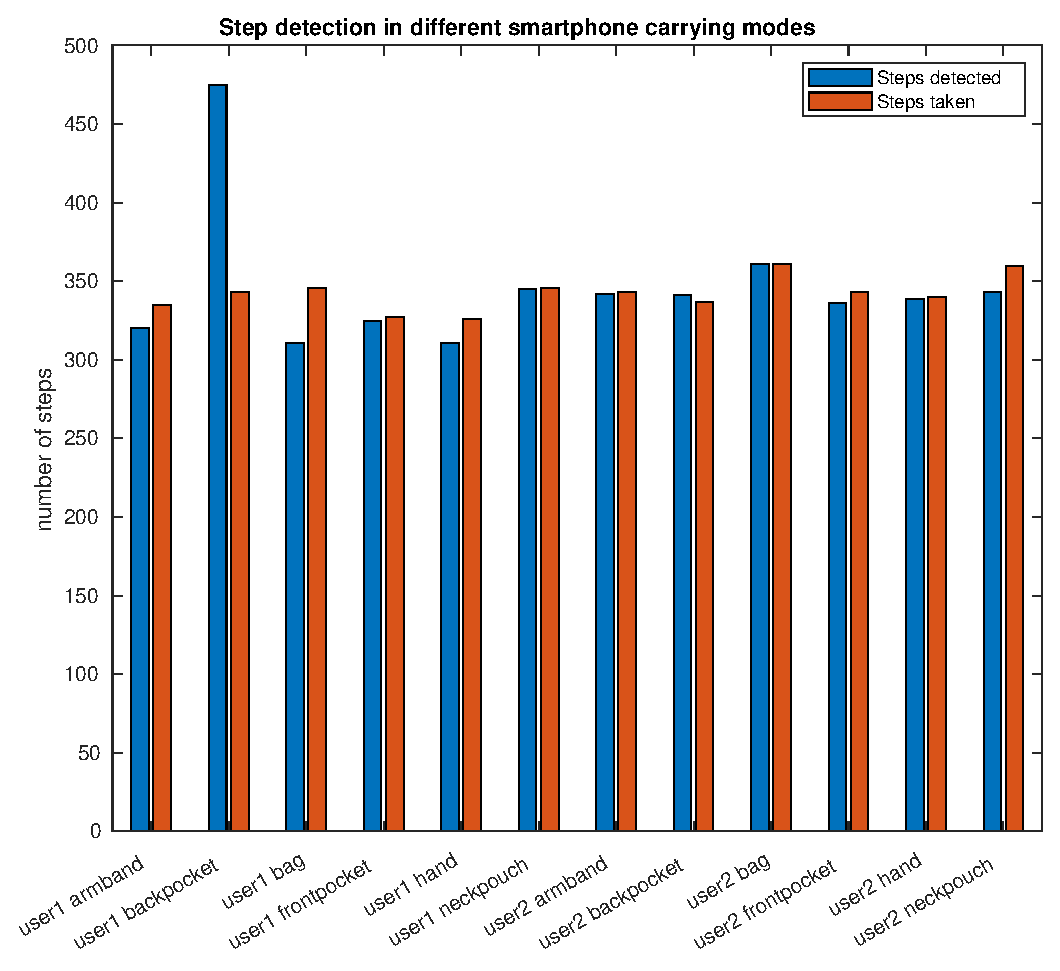
\includegraphics[width=0.7\linewidth]{images/20201127_1516_Step_detection_in_different_smartphone_carrying_modes}
		
		\caption{Absolute number of steps detected using method in \cref{sec:meth - step detection} on \citet{Brajdic2013} dataset.}
		\label{fig:sd_abs_comparison}
	\end{figure}
	\begin{figure}[H]
		\centering
		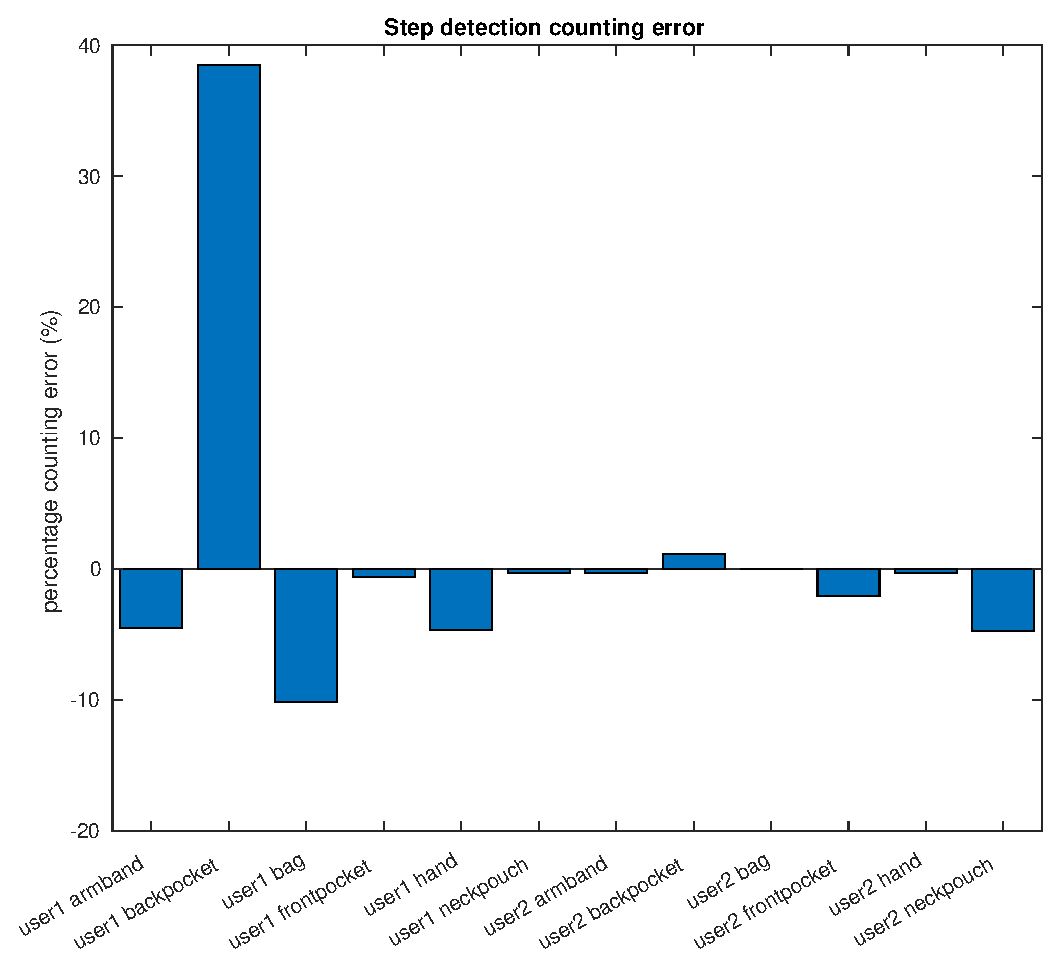
\includegraphics[width=0.7\linewidth]{images/20201127_1520_Step_detection_counting_error}
		\setlength{\belowcaptionskip}{-10pt}
		\caption{Percentage error step detections from steps taken using method in \cref{sec:meth - step detection}. }
		\label{fig:sd_percent_comparison}
	\end{figure}

%	\caption[Step detection comparison]{Comparison between \citet{Salvi2018} step detection algorithm, \cref{algo:step_detect} and ground truth for different carrying modes.}
%	\label{fig:sd_comparison}
\begin{figure}[H]
	\centering
	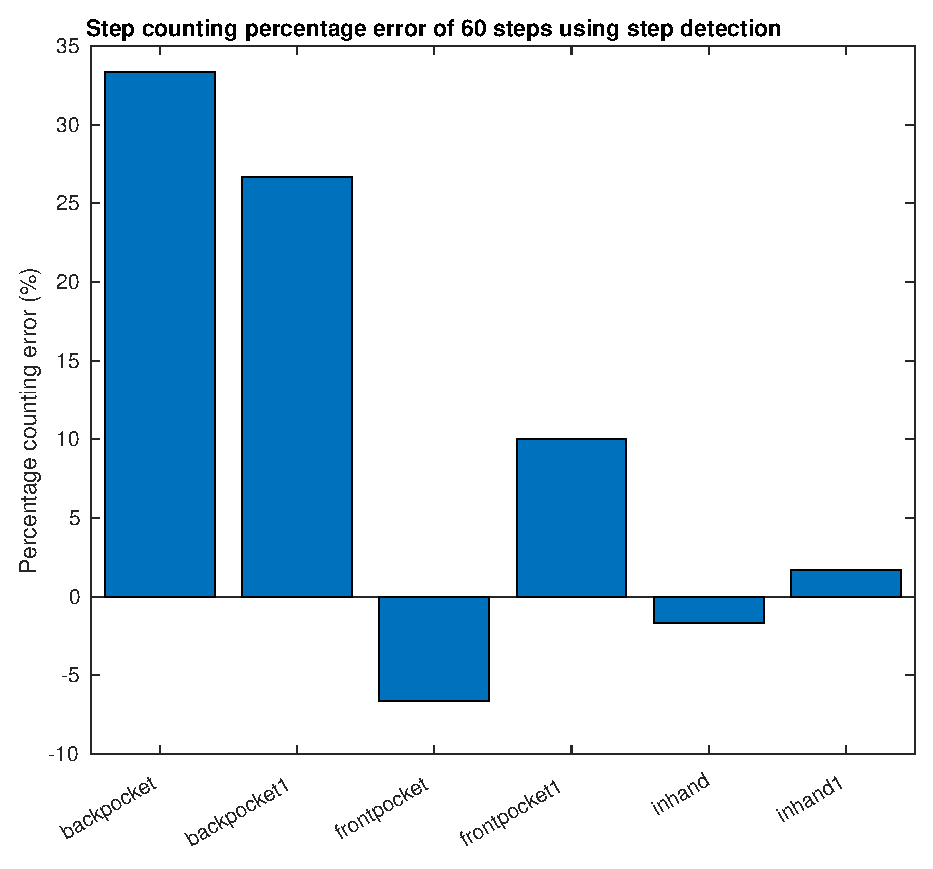
\includegraphics[width=0.7\linewidth]{images/20201127_1640_Step_counting_percentage_error_of_60_steps_using_step_detection}
	\setlength{\belowcaptionskip}{-20pt}
	\caption{Original data step counting using method in \cref{sec:meth - step detection} on \citet{Brajdic2013} dataset.}
	\label{fig:202009291013step_counting_error_of_60_steps}
\end{figure}

\subsection{Time Difference between Detection and Ground Truth Step}

For a \ac{SHS} it is not enough for the number of steps detected to be accurate, but also the time when a step actually occurs. Detecting a step, combined with the heading orientation at that moment, determines the displacement vector. It is therefore preferable for a detection to be as close as possible to when a step actually occurs, with no other detections in the vicinity. \par
Using the \citet{Salvi2018} data with ground truth step detection, the time difference between a step detection and its closest ground truth point was calculated per trial. The mean and standard deviation of the time difference for each carrying mode was calculated, shown in \cref{fig:202011130914smallest_diff_to_gt_1}. 

\begin{figure}[H]
	\centering
	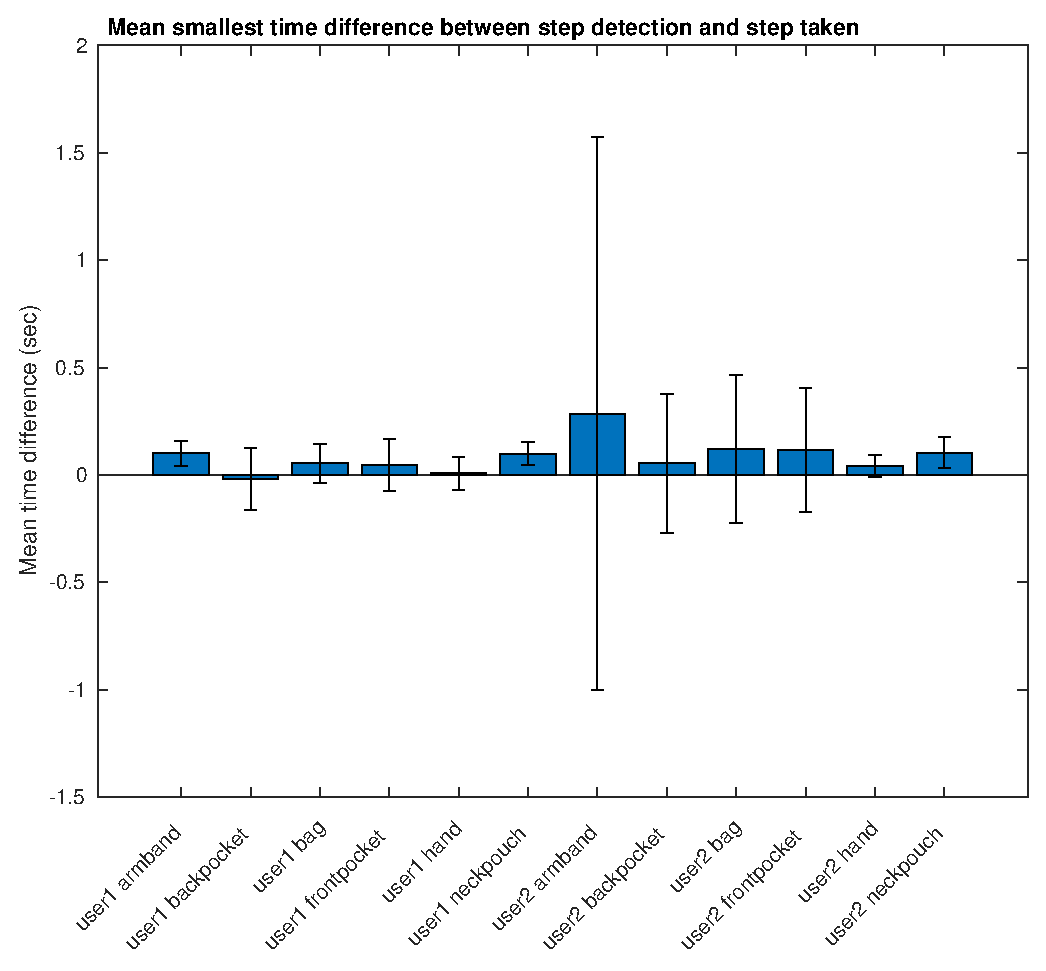
\includegraphics[width=0.7\linewidth]{images/20201127_1607_Mean_smallest_time_difference_between_step_detection_and_step_taken}
	\caption{Mean and standard deviation of the smallest time different between step detection and step occurrence using method in \cref{sec:meth - step detection} on \citet{Brajdic2013} dataset . Positive difference indicates detection before step occurrence and negative after occurrence}
	\label{fig:202011130914smallest_diff_to_gt_1}.
\end{figure}

The results show that most detections are within 0.1 seconds from the closest ground truth point. The best performing carrying mode is in hand. The large standard deviations for "user2 armband" is caused by the step detection methods having already counted multiple steps before the ground truth device has registered any. The low time difference for the backpocket carrying mode supports the hypothesis that double counting is occur close to step, since the time differences to the actual steps are small.

\subsection{Unique Step Detection}

One problem with time difference between detections and step taken is that two subsequent detections may have the same ground truth point as the nearest point, indicating that there is no unique detection of the step occurring. \par 

An approach to determining unique step detection performance was fashioned. Since it is unrealistic to expect the step detection to be at the exact time an actual step occurs, intervals are defined around ground truth step where if it is detected once within the interval using the method in \cref{sec:meth - step detection}, the detection counts as a unique step. If in this interval two steps are detected, no unique step is indicated. The time interval is increased itteratively in an attempt to find the highest unique step counts. The results for each user and carrying mode can be found in \cref{fig:sd_tp_fp_comparison}. 

\begin{figure}[H]
	\centering
	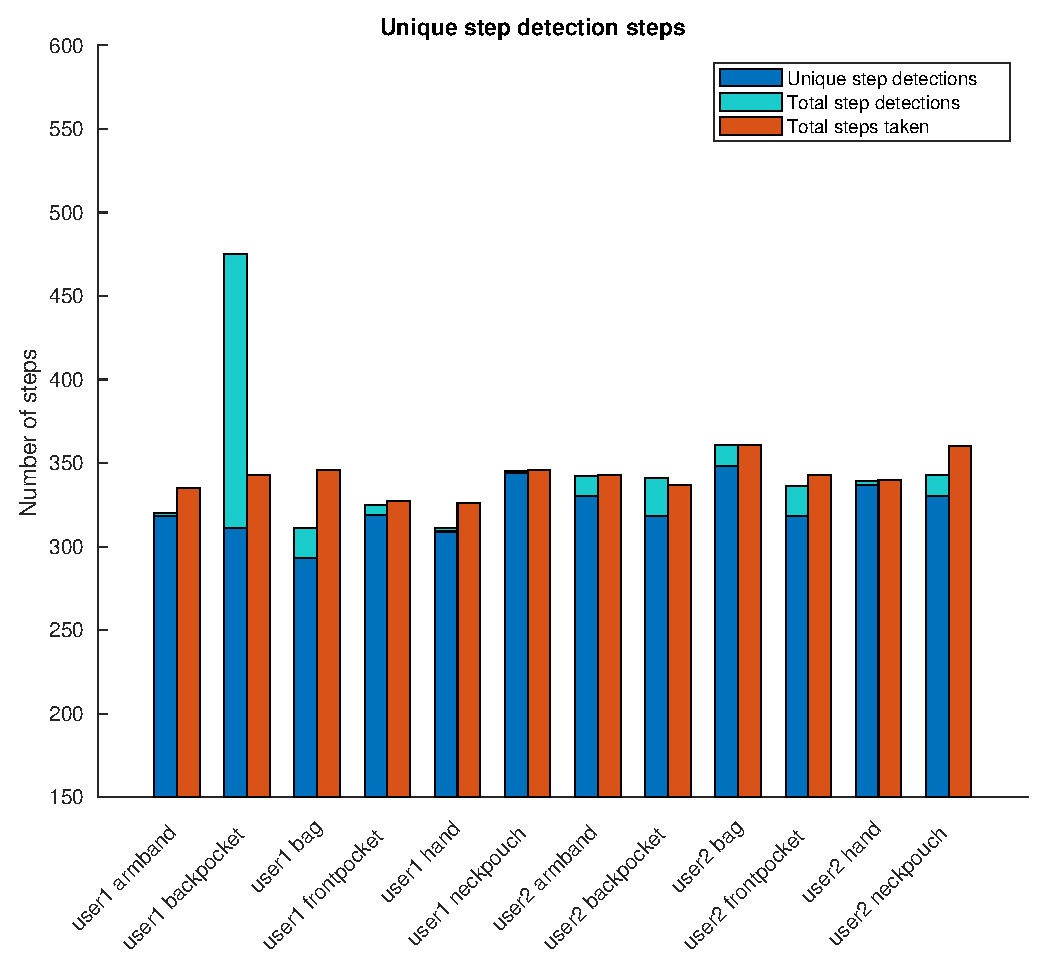
\includegraphics[width=0.7\linewidth]{images/20201127_1626_Unique_step_detection_steps}
	\setlength{\belowcaptionskip}{-10pt}
\caption[False positives and true positives step detection comparison]{Highest unique steps detected using interval method vs total number of steps taken using the method in \cref{sec:meth - step detection}. \citet{Brajdic2013} dataset is used. }
\label{fig:sd_tp_fp_comparison}
\end{figure}

These results show that the number of unique step is close to the total number of detections, indicating that the step detection method is relatively good at uniquely determining when steps are taken. \par 

From all results in step detection, the in front, in hand carrying mode has proven to be the best with low total counting error, small time difference to ground truth step and little to no double detections of the same step. This is likely caused by the fact that when held in hand, the smartphone is more or less attached to the user and has little possibility to wiggle in its constraints, in contrast to when the device is placed in pockets. It is fortunate that this carrying mode works best, since it also the carrying mode used for pedestrian heading estimation when testing the whole system.

\section{Step Length Estimation}
\label{sec:results-step_length_estimation}
For step length estimation, the linear relationships between dependent variables and step length, outlined in \cref{sec:rw - step detection} need to be determined using step detection method in \cref{sec:meth - step detection}. The step detection algorithm cannot guarantee that all steps are counted, potentially affecting the tunable parameter for both methods.  From \cref{sec:rw - step detection} the best performing algorithm for global parameters according to \cite{Vezocnik2019} is reiterated for convenience,

\begin{equation}
	\label{eq:Tian2016_sle2}
	\text{step size} = K_1 h \sqrt{F}.
\end{equation}


where $h$ is the user's height and $F$ is the step frequency. The linear relationship between step length and the dependent variables is defined by $ K_1 $, a tunable parameter. \par 

The best algorithm for individual parameters is 

\begin{equation}
	\text{step size} =K_2 \sqrt[4]{A_{\max }-A_{\min }},
	\label{eq:weinberg_stepsize2}
\end{equation}

where $A_{\max}$ and $A_{\min}$ are the maximum and minimum acceleration within a step interval. The two approaches will be used and compared to see if similar results are achieved as within \cite{Vezocnik2019}.

\citet{Vezocnik2019} have made their accelerometer data available under an open license, consists of smartphone accelerometer data of 15 different people for three walking speeds and in different carrying modes, including in front of the torso and in hand with the screen pointing up. This carrying mode will be used for step length estimation in this section, since it performed best in step detection and is used for heading estimation. \par 
Within the dataset metrics for each test subject are collected, including height, gender, and leg length. The walking speeds were defined qualitative, in that they were either slow, normal, or fast. Each person has two measurements for each walking speed, one for a 15-meter long straight path and another for a 108-meter long straight path. Within \cite{Vezocnik2019}, the smaller set is used to determine parameters for step length estimation methods, while the longer distance is used as a performance measure. This same process will be used to determine the performance of step detection and step length estimation.First the tuneable parameters $ K_1$ and $ K_2$ will be determined using the shorter length walking distances in the opensource data. \par 

\subsection{Parameter Estimation}

In \cref{fig:step_length_tian}, the dependent variables of \eqref{eq:Tian2016_sle2} are plotted against average step length. The data from the smaller distances in the \citet{Vezocnik2019} dataset are used. The average step length is calculated by dividing the distance traveled by the number of steps detected. In the figure each test subject is shown as a different color with the form of the different markers indicating the speed at which that trial was walked at. The positive upward trend indicated in \eqref{eq:Tian2016_sle2} can be observed for all test subjects as walking speed increases. In order to find the universal constant $K_1$ in \eqref{eq:Tian2016_sle2}, a linear least square estimation is performed across all test subject data points. The result is shown by the green striped line in \cref{fig:step_length_tian}, where $ K_1 = 0.3116$. \par 

A similar plot is shown in \cref{fig:step_length_weinberg}, using the same data as in \cref{fig:step_length_tian} but for the \eqref{eq:weinberg_stepsize2} dependent variables. The positive trend indicated by \eqref{eq:weinberg_stepsize2} can be noticed. Since \eqref{eq:weinberg_stepsize2} works best for personalized variable the tunable parameter $ K_2 $ is calculated per test subject, instead of all together as with \eqref{eq:Tian2016_sle2}. This is also done through the linear least square approach.

	\begin{figure}[H]
	\centering
	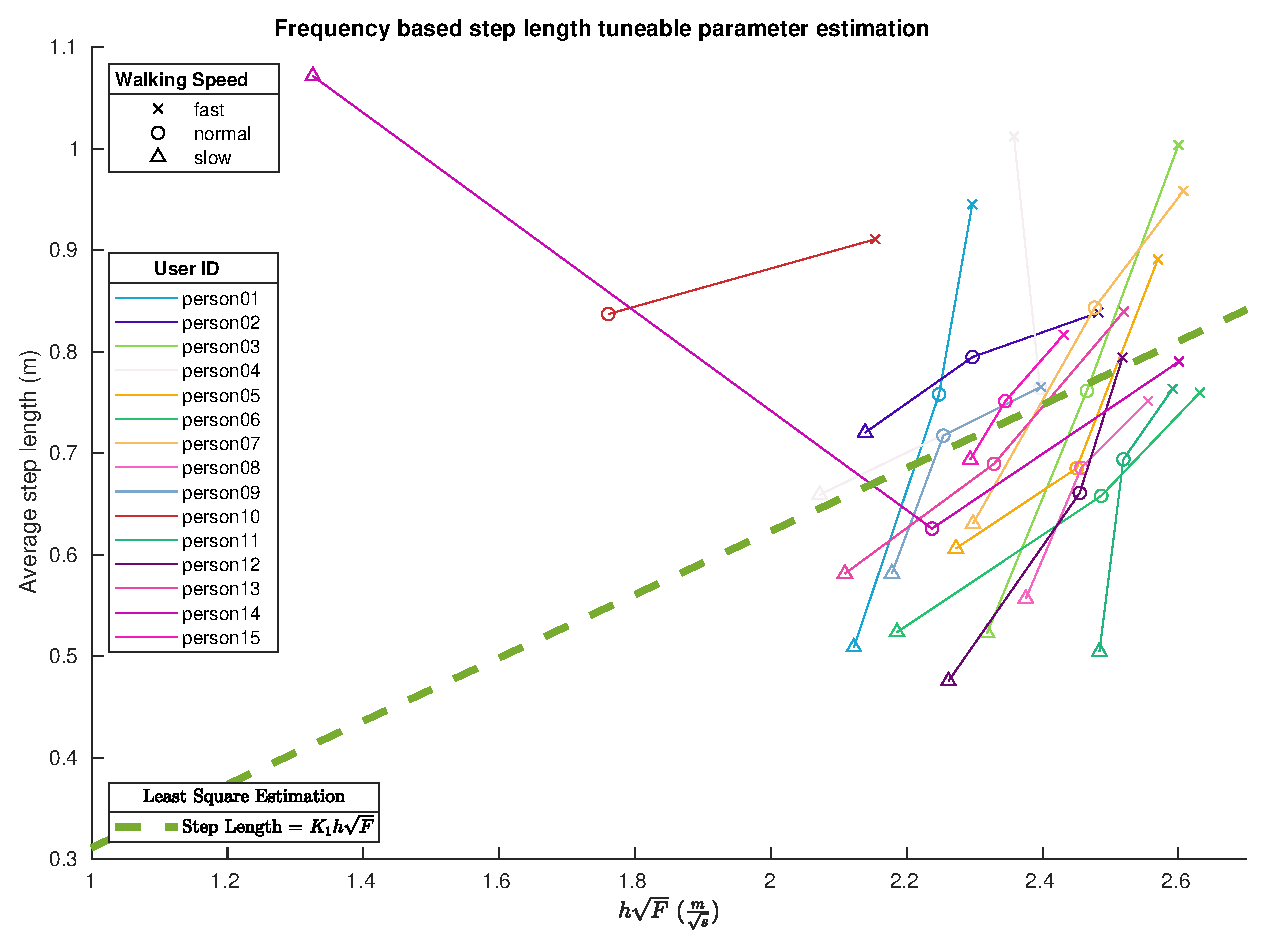
\includegraphics[width=0.8\linewidth]{images/20201128_1304_}
	\caption{Dependent variables of \eqref{eq:Tian2016_sle2} plotted against average step length over the smaller distances in the \citet{Vezocnik2019} dataset with step detection from \cref{sec:meth - step detection}. Green striped line represents \eqref{eq:Tian2016_sle2}, where $ K_1 = 0.3116$.  }
	\label{fig:step_length_tian}
	\end{figure}

\begin{figure}[h]
	\centering
	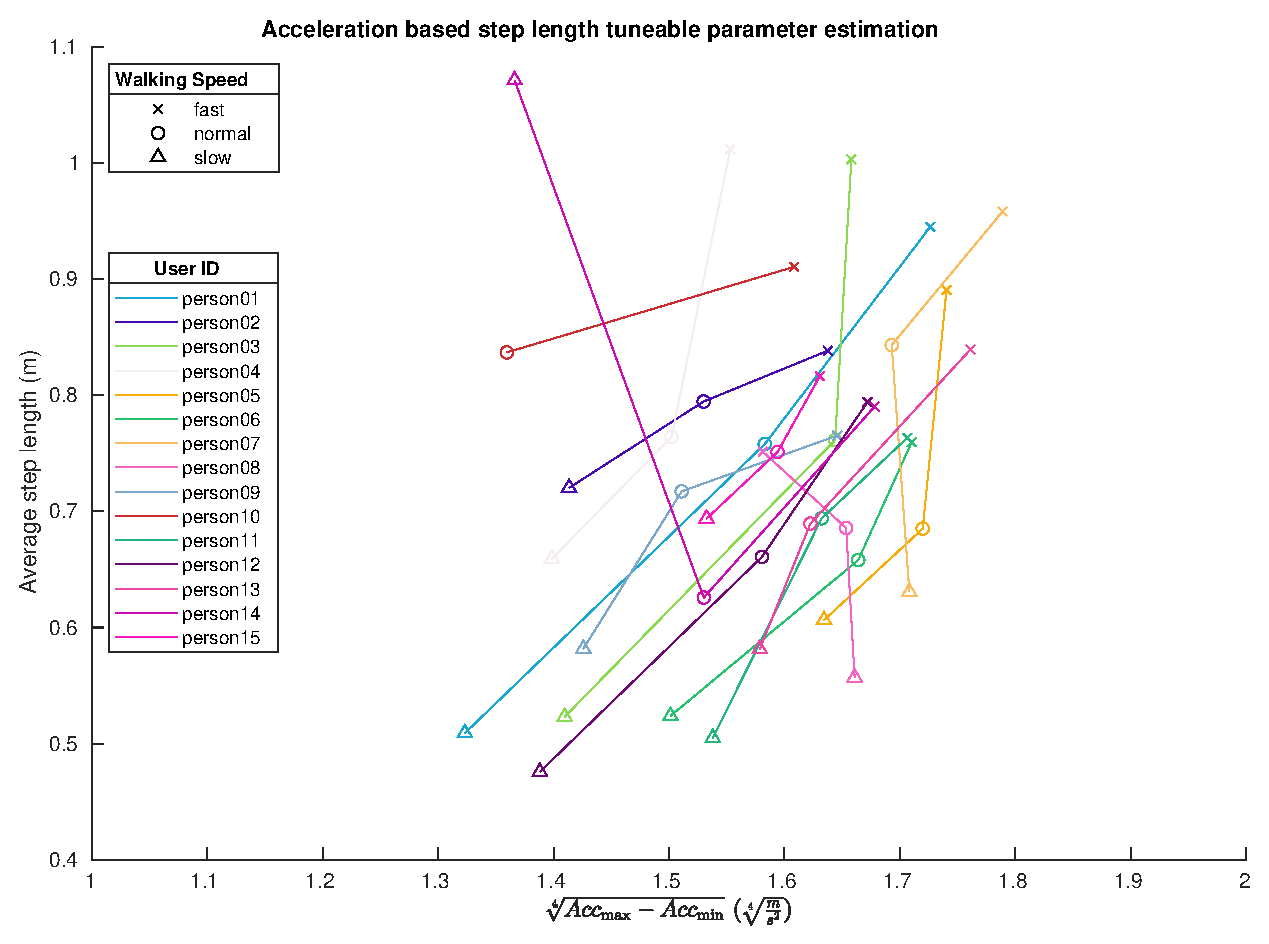
\includegraphics[width=0.8\linewidth]{images/20201128_1317_}
	\caption{Dependent variables of \eqref{eq:weinberg_stepsize2} plotted against average step length over the smaller distances in the \citet{Vezocnik2019} dataset.}
	\label{fig:step_length_weinberg}
\end{figure}

While most data seems to follow the general linear relationship for both approaches, there are two samples that do not. The two potentially faulty data points are the slow walking sample of both person 10 and 14. For the former, no steps have been detected and are therefore not visible in the plots, while for the latter too few steps have been detected. \par 

For person 14, 14 steps have been detected for slow walking, which is fewer steps than when the subject was walking fast. This is either a wrong step detection occurring, or the user walks slowly with very large steps. It is difficult to determine why this is occurring. It could be that during this sample, the test subject was holding the phone incorrectly, the person had a very different step strategy when performing at this speed, or the phone was malfunctioning. \par 

This outlier affects the eventual tunable parameter for both step length approaches. Removing it will change the estimate of $K_1$ from 0.3116 to 0.3080. The validation dataset can be used to determine if the difference in the tunable parameter has a significant effect on the total distance traveled. The difference was found to have a negligible effect on the outcome of the method.
%The results are found in  \cref{fig:step_length_estimation_validation}, where the absolute distance error for all walking speeds for all test subjects are shown, indicated by the dataset ID.
%\begin{figure}[H]
%	\centering
%	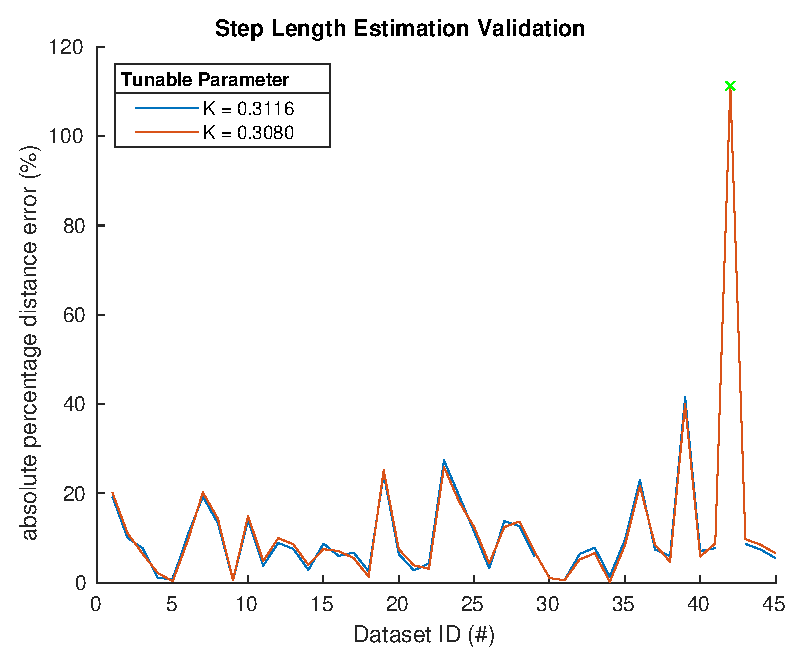
\includegraphics[width=0.65\linewidth]{images/20201028_1344_Step_Length_Estimation_Validation}
%	\setlength{\belowcaptionskip}{-30pt}
%	\caption{Step length estimation using validation dataset}
%	\label{fig:step_length_estimation_validation}
%\end{figure}

\subsection{Step Length Method Validation}

The performance of both step length estimators is evaluated by applying them to the data of the longer walking distance in the \citet{Vezocnik2019} dataset. The estimated total distance from both \eqref{eq:Tian2016_sle2} and \eqref{eq:weinberg_stepsize2} can be compared with the actual distance walked. The results are shown in  \cref{fig:202011131943_wienberg_vs_tian_vezocnik_data1}. This data surprisingly shows that depending on the test subject one or the other method is better at estimating distance traveled at different walking speeds. This does not coincide with the results of \cite{Vezocnik2019}, where \eqref{eq:weinberg_stepsize2}, which uses personalized parameters for $ K_2 $, performed better than \eqref{eq:Tian2016_sle2}, which uses general parameters for $ K_1 $. \par 

What is noticeable from the results is that there is an outlier. This is with the slow walking speed of test subject 14, which is are also the test subject with which the tunable parameter estimation had an outlier. This further supports that there is something significantly different when this test subject is performing at this walking speed.\par 

 Without the outlier, the mean absolute error for \eqref{eq:Tian2016_sle2} method is 9.7 percent with a standard deviation of 8.0 percent. For the \eqref{eq:weinberg_stepsize2} method the mean is 10.38 percent error with a standard deviation of 7.8 percent error. Both results differ from those cited by \cite{Vezocnik2019}, which indicate a mean of 7 percent with a standard deviation of 5 percent for the former and 3 percent with a 2.5 percent standard deviation for the latter.
 This is most likely caused by the difference in step detection methods, which \cite{Vezocnik2019} does not state explicitly.
 
\par

\begin{figure}[]
	\centering
	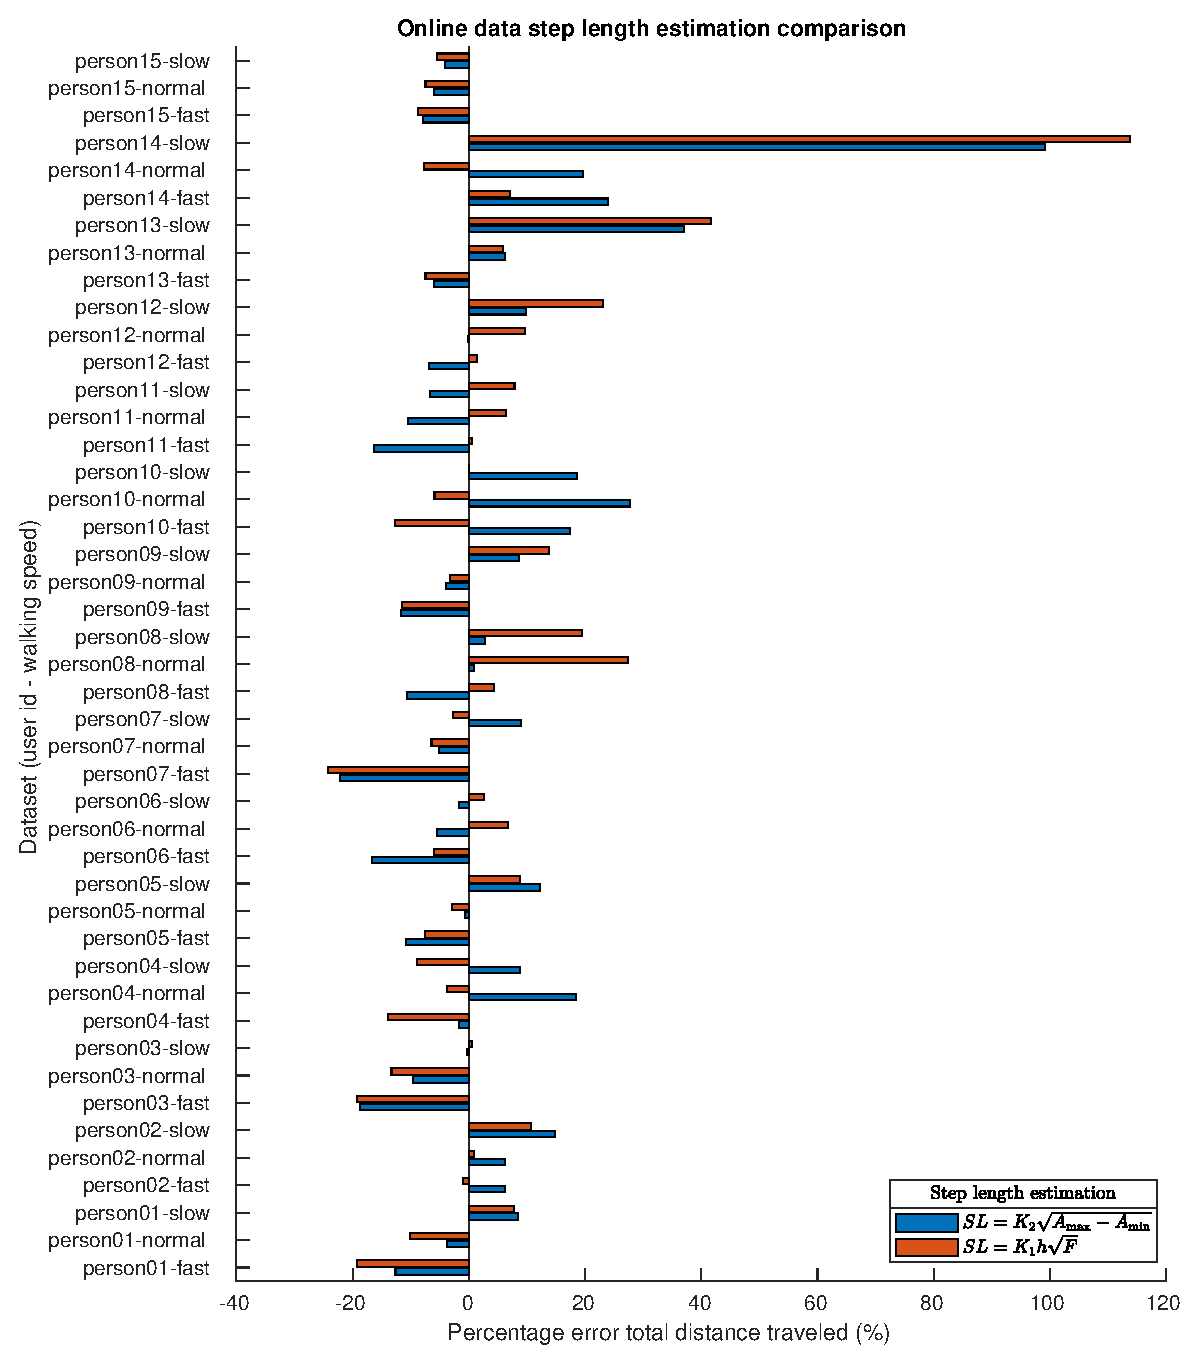
\includegraphics[width=\linewidth]{images/20201128_1403_Online_data_step_length_estimation_comparison}
	\caption{Total distance traveled estimation error from in front, in hand carrying mode from long distance data from \citet{Vezocnik2019} dataset, using \eqref{eq:Tian2016_sle2} and \eqref{eq:weinberg_stepsize2} with step detection from \cref{sec:meth - step detection}. }
	\label{fig:202011131943_wienberg_vs_tian_vezocnik_data1}
\end{figure}
 
Since no conclusive result could be distilled from applying the methods to the opensource data, a small scale experiment was performed outdoors. Within the experiment the same process as in \cite{Vezocnik2019}, where a small distance was used for parameter $ K_1 $ and $ K_2 $ estimation and a longer for performance measurement. Original data was collected from the same person and device used in the eventual indoor localization experiment. The smartphone was held in front of the torso and in hand as in \cref{fig:experiment_carrying_position}. \par 

Three trials of 30 meters were walked at different qualitative walking speeds, slow, normal, and fast, while recording accelerometer data. Four longer trials of 300 meters were walked, to determine performance, also at different walking speeds. All trials were walked with the smartphone in the same carrying mode. \par 

During the smaller walking distances, the number of steps taken was counted manually. For two trials the number of steps detected was exactly the number of steps taken. This was for slow and fast walking where 67 and 50 steps were counted respectively.  For the other trial, the detection was off 2 steps, with 57 steps being taken and 55 being recorded. With these results indicating that step detection is working properly, errors in step length estimation is likely not caused by wrongful step detection.  \par 

The different step length estimation methods were applied to the original accelerometer data. The same parameter $ K_1 $ determined for the online dataset. The $ K_2 $ parameter was based on the smaller distance data. The results are shown in \cref{fig:step_length_personal_testing}. The results suggest that for slow to normal walking step detection using \eqref{eq:Tian2016_sle2} works best, with a chance of underestimating the distance traveled. For normal to fast walking using \eqref{eq:weinberg_stepsize2} for step detection works better, with a chance of overestimating the distance traveled. By making the assumption that walking indoor is generally more in the normal to slow speed range, the choice was made to use the \eqref{eq:Tian2016_sle2} method for step length estimation in the indoor localization system.
\begin{figure}[H]
	\centering
	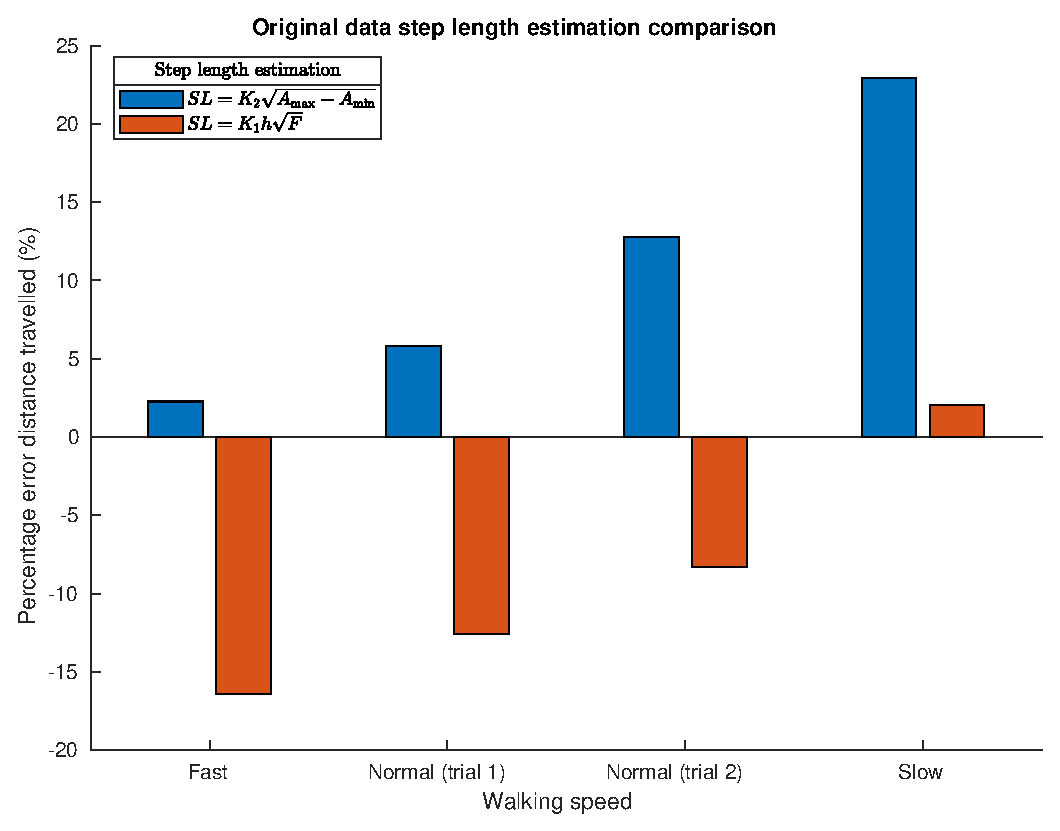
\includegraphics[width=0.7\textwidth]{images/20201128_1430_Original_data_step_length_estimation_comparison}
		\setlength{\belowcaptionskip}{-15pt}
	\caption{Step length estimation method comparison using original accelerometer data recording while walking and step detection from \cref{sec:meth - step detection}. }
	\label{fig:step_length_personal_testing}
\end{figure}

For both the opensource data and the original data the accelerometer based method in \eqref{eq:weinberg_stepsize2} does not necessarily work better than frequency based method in \eqref{eq:Tian2016_sle2}, as indicated by \citet{Vezocnik2019}. For future work it may be worthwhile to test the other algorithms outlined by \cite{Vezocnik2019} to see if there are any other differences between the outcomes. 

\section{Indoor Orientation Estimation}

Determining the performance of orientation estimation during the indoor experiments is difficult since no ground truth was available for comparison. A sanity check that can be performed is comparing the orientation estimations of the EKF with the orientation estimations calculated by the android operating system. The results will not be able to give an indication of which performed best with respect to reality, but could potentially highlight any very diverging behavior. \par 

In order to calculate an orientation difference, a difference quaternion ($	\Delta q_t$) can be used, defined as \cite{Kok2017}

\begin{equation}
	\Delta q_t = \hat{q}_{t}^{nb} \odot \left( \hat{q}_{comp,t}^{nb}  \right)^c,
\end{equation} 

where $\hat{q}_{comp,t}^{nb}$ is the unit quaternion that $ \hat{q}_{t}^{nb} $ is compared with.  In order to compare the orientation estimates of the android system and the EKF from \cref{algo:indoor_EKF}, the difference in angle between the first quaternion estimate and the following quaternions estimate is calculate for both orientation estimates. This is done to calculate the relative orientation estimate to the initial orientation, which are the angles used by the \ac{SHS}.\par 

Since both relative orientation estimates start at the same initial quaternion, the two estimates can now be compared. Applying the difference quaternion calculation to these estimates, the difference quaternions over the whole orientation estimate are determined.  \par 

Once calculated, the difference quaternions can be converted into Euler angles for more intuitive interpretation. The mean difference in yaw component for each trial is shown in  \cref{fig:yaw_difference_between_android_and_ekf_1}. From the results, the difference between both orientation estimations seems larger for trial 3 and 6, requiring further investigation.

\begin{figure}[H]
	\centering
	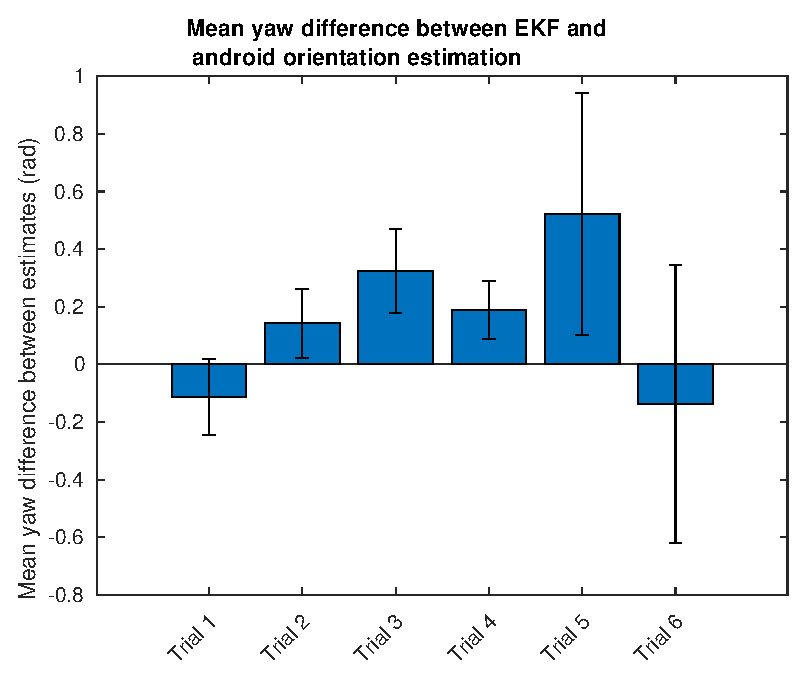
\includegraphics[width=0.7\linewidth]{images/20201128_1646_mean_yaw_difference_1}
	\setlength{\belowcaptionskip}{-20pt}
	\caption{Mean yaw difference between \cref{algo:indoor_EKF} and android orientation estimates.}
	\label{fig:yaw_difference_between_android_and_ekf_1}
\end{figure}

\newpage
\section{Step and Heading System Particle Filter Testing}

Through the indoor experiment outlined in \cref{sec:results-experimental setup} the complete indoor localization system could be tested from input sensor measurements and map information to postion estimate. The IMU data is passed through the \ac{SHS} subsystem of \cref{sec:method-SHS} to produce a \ac{SHS} trajectory. The smartwatch IMU data is passed through the activity recognition method in \cref{sec:method-AR} to  detect door interaction. Combining the \ac{SHS} trajectory and door interaction detection with the floor map generated in \cref{sec:method-particle_filter}, the Particle Filter propagates position estimates through the indoor environment, while taking spatial context into account. The resulting trajectories from the particles at the last time step of the SHS are averaged to produce the indoor position estimate over the experiment , as explained in \cref{sec:method-pf_location_estimate}. The whole system combined will be referred to as the Step and Heading Particle Filter (SHS-PF).  \par 

By using the video recordings made during the different trials, a rough position trajectory was created. This rough estimate can be used for comparison with the position estimate of the \ac{SHS} Particle Filter, in order to get an indication of the estimating performance. This can be done by calculating the root-mean-square error between the two position estimate as

\begin{equation}
	\displaystyle \operatorname {RMSE} ={\sqrt {\frac {\sum _{t=1}^{T}({\hat {y}}_{t}-y_{t})^{2}}{T}}},
	\label{eq:RMSE}
\end{equation}

where $T$ is the total time of the trial, $\hat{y_t}$ the postion estimate at time $t$ of the SHS-PF and $y_t$ the video trajectory position at time $t$.

\subsection{SHS-PF with Manually Labeled Door Interaction}
\label{sec:results-SHS_PF_manually indicated}
During the experiment, timestamps were recorded to indicate the beginning of interaction with a door within the indoor environment. The recorded timestamps can be used to trigger a Particle Filter door interaction measurement update. Using this method, the potential effect of activity recognition for indoor localization in the ideal case can be evaluated, since there is no chance for false positives to occur.\par

This section will first use these additional position measurements to find model parameters, through an iterative process. First the number of particles to use will be estimated. Afterwards the standard deviations in the time update of the Particle Filter will be determined. Once these parameters are defined, the performance of SHS-PF with manually labeled door interaction is evaluated.

\subsubsection{Determining Particle Filter Time Update Standard Deviations}

\subsubsection{Determining Number of Particles}

This represent particle runs that have been able to propagate particles for the whole \ac{SHS} trajectory.
 
\begin{figure}[H]
	\centering
	\begin{subfigure}[t]{.38\textwidth}
		\centering
		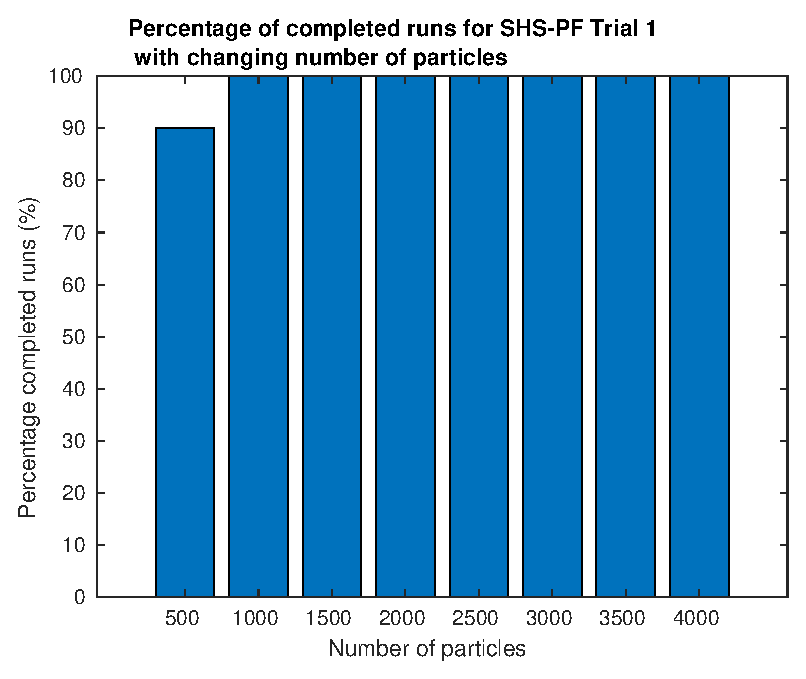
\includegraphics[width=\linewidth]{images/20201129_1147_Trial_1_nr_particles_1}
		\caption{}
		\label{fig:trial1_nr_particles}
	\end{subfigure} \quad
	\begin{subfigure}[t]{.4\textwidth}
		\centering
		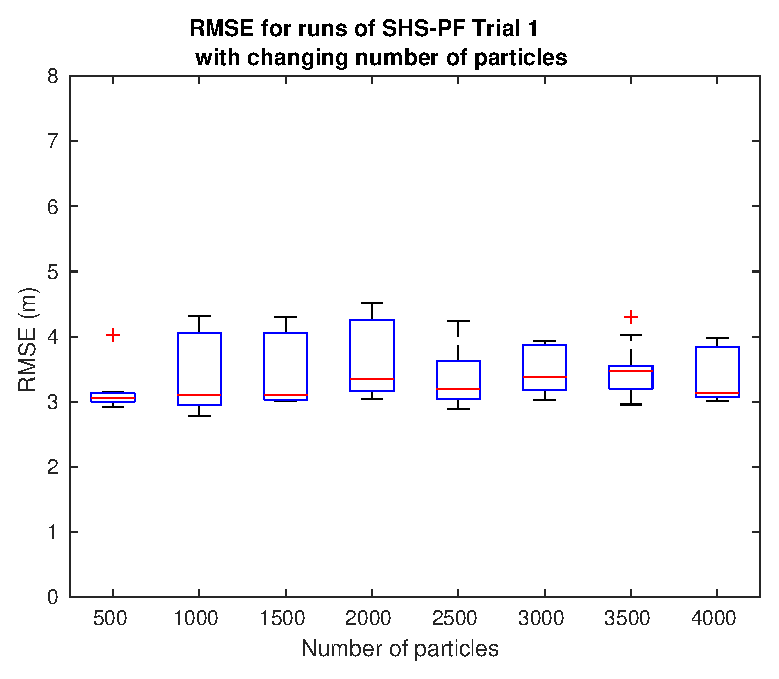
\includegraphics[width=\linewidth]{images/20201129_1154_Trial_1_RMSE_nr_particles_1}
		\caption{}
		\label{fig:trial3_nr_particles}
	\end{subfigure} \quad
\end{figure}

\begin{figure}[H]
	\centering
	\begin{subfigure}[t]{.4\textwidth}
		\centering
		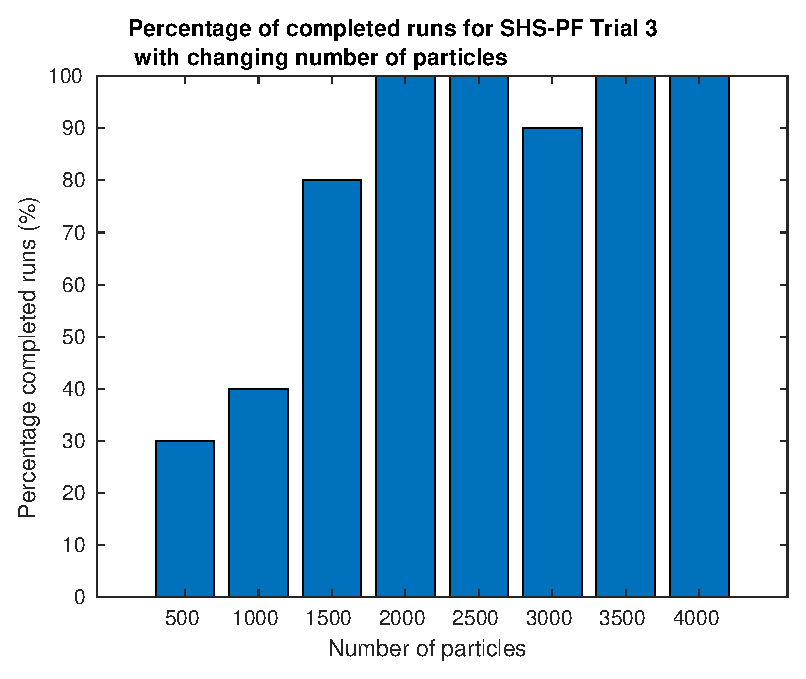
\includegraphics[width=\linewidth]{images/20201129_1147_Trial_3_nr_particles_1}
		\caption{}
		\label{fig:trial3_nr_particles}
	\end{subfigure} \quad
\begin{subfigure}[t]{.4\textwidth}
	\centering
	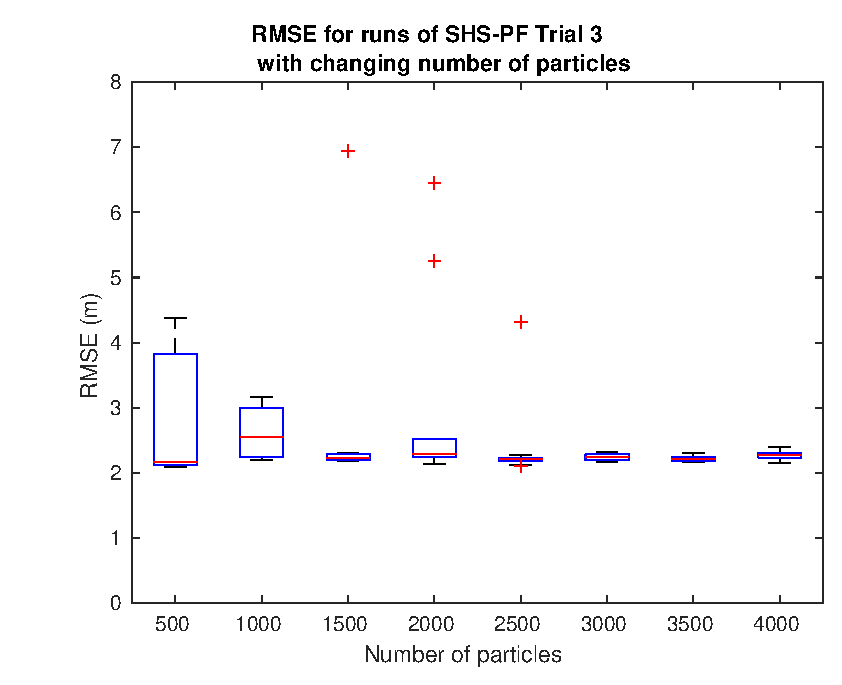
\includegraphics[width=\linewidth]{images/20201129_1154_Trial_3_RMSE_nr_particles_1}
	\caption{}
	\label{fig:trial3_nr_particles}
\end{subfigure} \quad
\end{figure}

\subsubsection{Performance}
All trials were run through the complete SHS-PF with the manually recorded door interactions, with 4000 particles. This was done for five runs per trial, in order to show reproducibility. The results can be found in \cref{fig:pf_boxplot}. The figure shows the root-mean-square errors values per experimental trial over 5 runs. At the top of the figure the amount of completed runs is indicated.

\begin{figure}[H]
	\centering
	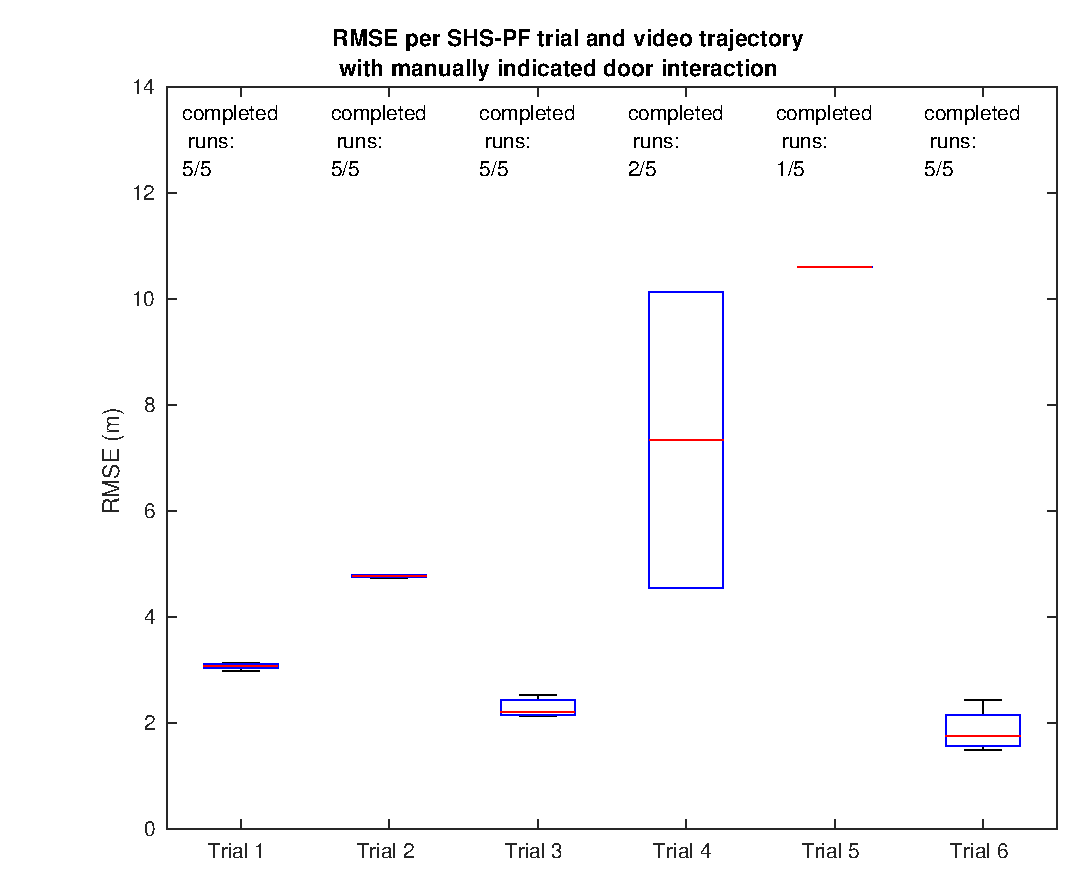
\includegraphics[width=0.7\textwidth]{images/20201129_1419_RMSE_manually_indicated_ar_shspf_trials_1}
	\caption[Particle Filter position estimation performance with manual door interaction]{Particle Filter position estimation root mean square error compared to rough video generated estimate. Manually indicated door interactions were used for Particle Filter measurement update.}	
	\label{fig:pf_boxplot}
\end{figure}

The results show that for trials 1 to 3 and trial 6 that all five runs were completed, with their individual runs having similar RMSE values to the rough video estimate. The RMSE value per trial do vary, which can be explained by looking at the trajectory that the system generates. \par  

While the particles for trial 1 and 2 complete all iterations, however both do not follow the complete trajectory derived from video analysis. This can be seen in  \cref{fig:shspf_trial1_shs_gt_comparison} where the structure circled in green is circled by the rough estimate but not by the Particle Filter. For \cref{fig:shspf_trial2_shs_gt_comparison} the Particle Filter seems to walk too far and is unable to make the correct turn.

\begin{figure}[H]
	\centering
	\begin{subfigure}[t]{.45\textwidth}
		\centering
		\begin{tikzpicture}
			\node[anchor=south west,inner sep=0] (image) at (0,0) {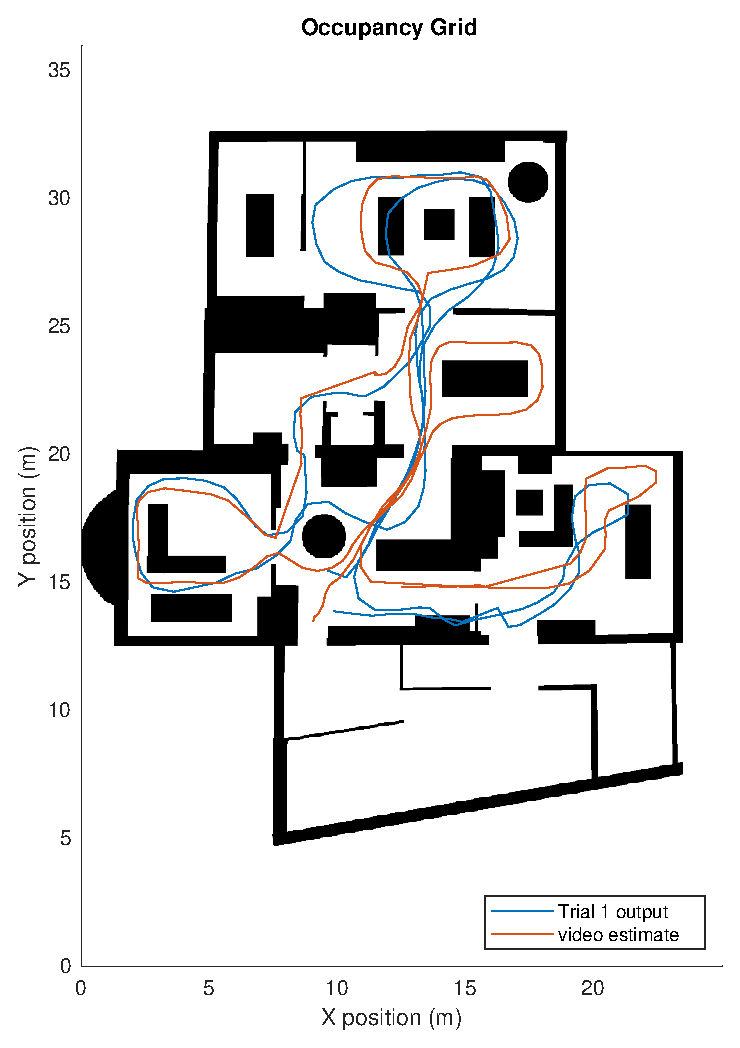
\includegraphics[width=0.9\textwidth]{images/20201118_1900_trial1_output_2}};
			\begin{scope}[x={(image.south east)},y={(image.north west)}]
				\draw[green,ultra thick,rounded corners] (0.6,0.625) rectangle (0.73,0.66);
			\end{scope}
		\end{tikzpicture}		
		\caption{trajectory comparison}
		\label{fig:shspf_trial1_on_map}
	\end{subfigure}
	\begin{subfigure}[t]{.45\textwidth}
		\centering
		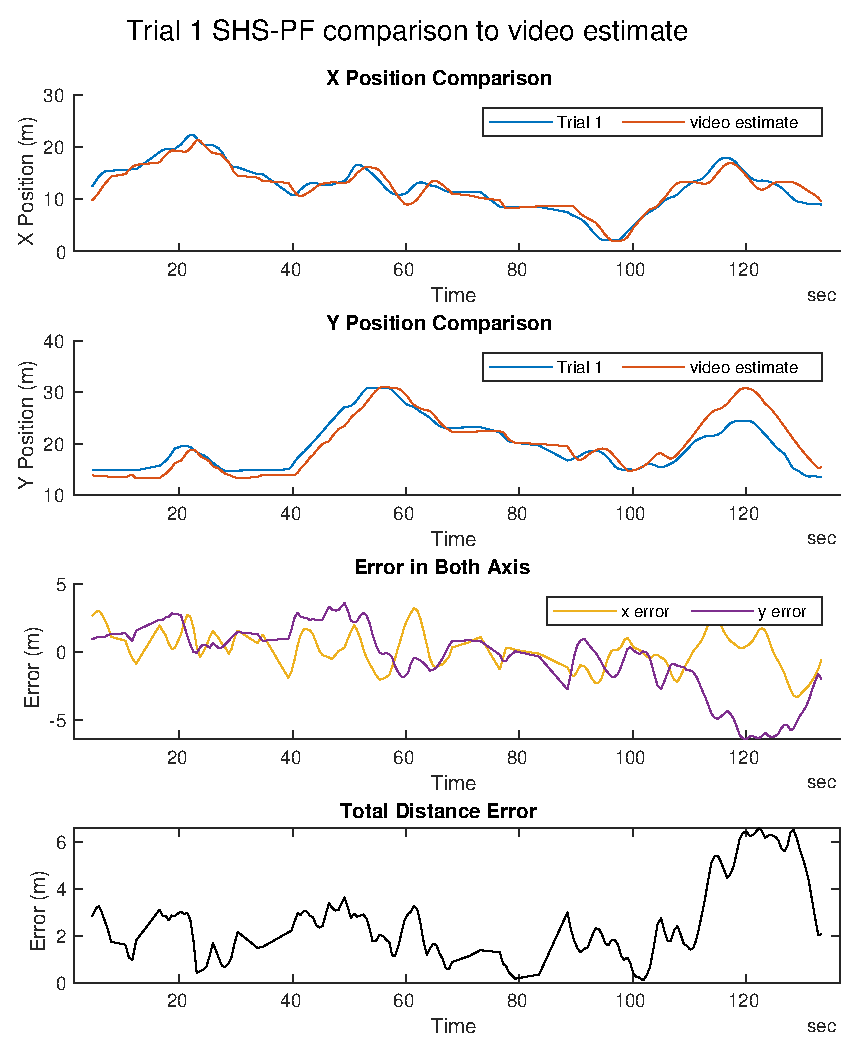
\includegraphics[width=\linewidth]{images/20201118_1900_trial1_output_1}
		\caption{axis comparison}
		\label{fig:shspf_trial1_comparison}
	\end{subfigure}
	\setlength{\belowcaptionskip}{-20pt}
	\caption{SHS-PF comparison of trial 1 with ground truth}
	\label{fig:shspf_trial1_shs_gt_comparison}
\end{figure}
\begin{figure}[H]
	\centering
	\begin{subfigure}[t]{.45\textwidth}
		\centering
		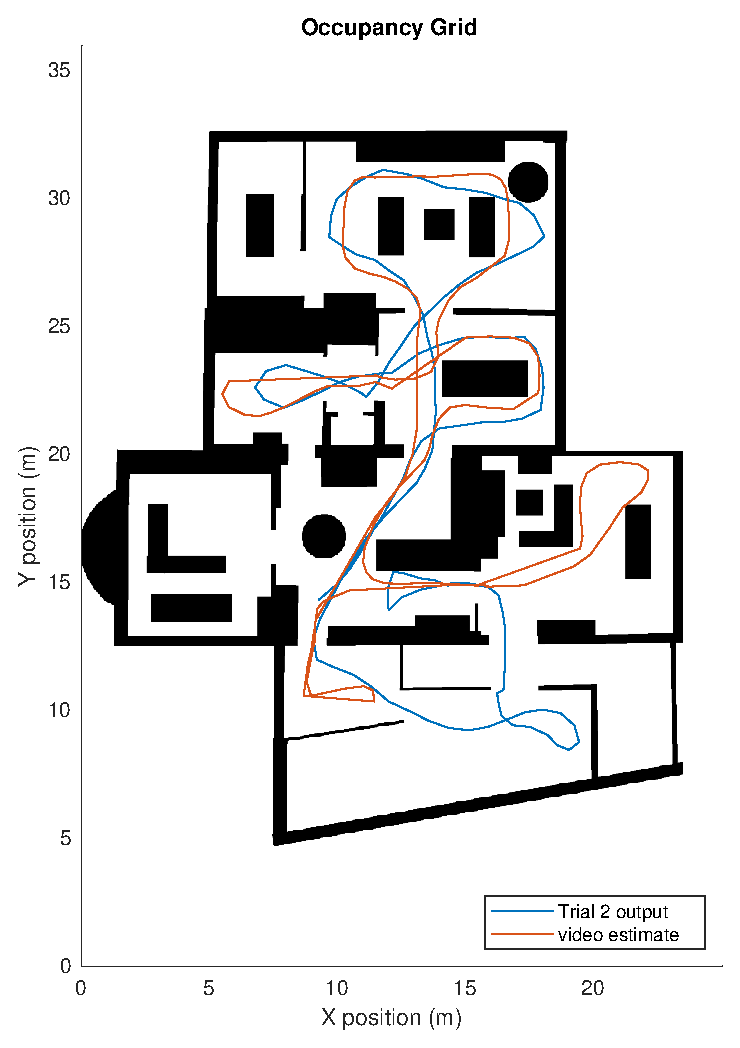
\includegraphics[width=0.9\linewidth]{images/20201118_1902_trial2_output_2}
		\caption{trajectory comparison}
		\label{fig:shspf_trial2_on_map}
	\end{subfigure}
	\begin{subfigure}[t]{.45\textwidth}
		\centering
		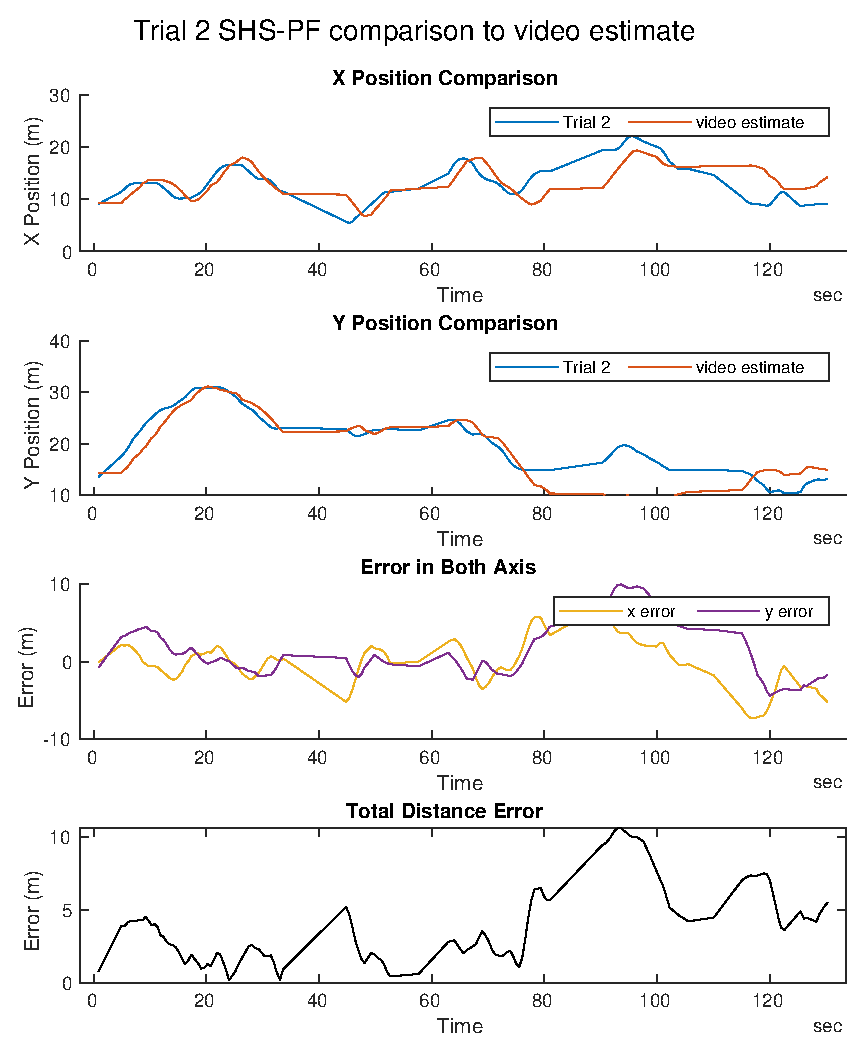
\includegraphics[width=\linewidth]{images/20201118_1902_trial2_output_1}
		\caption{axis comparison}
		\label{fig:shspf_trial2_comparison}
	\end{subfigure}
	\caption{SHS-PF comparison of trial 2 with ground truth}
	\label{fig:shspf_trial2_shs_gt_comparison}
\end{figure}

 Trial 3 and 7 are able to follow the route better. corresponding to lower RMSE values, the outputs are shown in \cref{fig:shspf_trial7_shs_gt_comparison}.
I have a hypothesis that step length estimation is overestimating distance traveled in some cases. This can be caused by turning not having the same displacement as a straight step.
Show a table of the distance walked according to rough video estimate and what the \ac{SHS}estimated.

Trials 5 and 6 are unable to complete any iteration reliably even with "perfect" activity recognition. This seems to suggest that the output of the \ac{SHS}is not good enough. This needs to be shown in figures.


The total SHS-PF solution was unable to get a reliable output for trials 4 and 5.\par 

\subsection{SHS- PF with Door Interaction Detection}
Applying the activity recognition method on the smartwatch data outline in Algorithm 3, door interactions could be detected. Using these detections instead of the manually indicated ones, the results in \cref{fig:rmse_per_trial_with_activity_recognition} were generated

\begin{figure}[H]
	\centering
	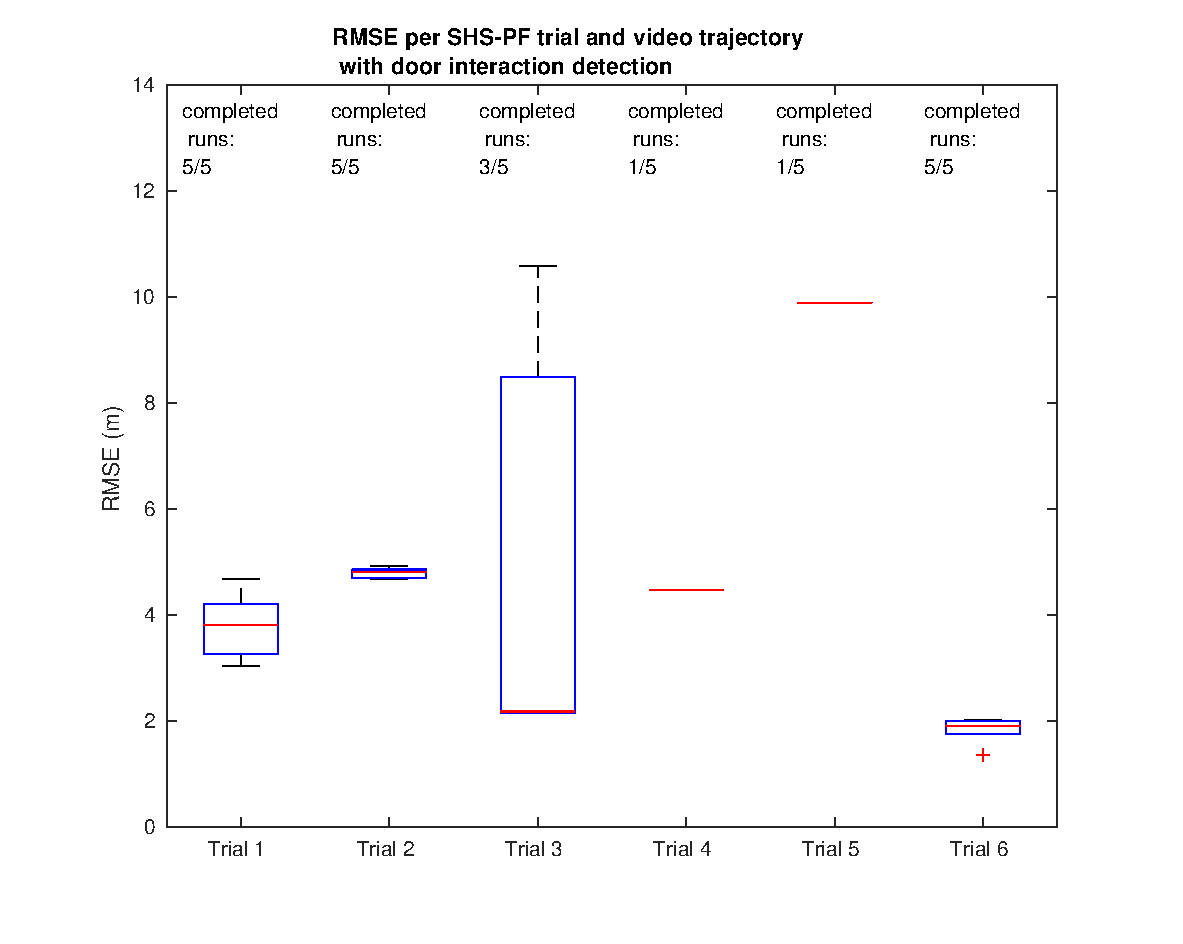
\includegraphics[width=0.7\linewidth]{images/RMSE_door_interaction_detections_ar_shspf_trials}
	\caption[Particle Filter position estimation performance with door interaction]{Particle filter position estimation root mean square error compared to rough video generated estimate using detected door interactions.}
	\label{fig:rmse_per_trial_with_activity_recognition}
\end{figure}

Trials 1,2 and 6 show similar results as when "perfect" activity recognition was used. Also the inability to complete all iterations for trials 5 and 6 is still present. In contrast trial 3 is also unable to complete all iterations, with the completed iterations leading to much larger RMSE values than before. 

\subsection{SHS-PF without Door Interaction Measurement Update}
In order to see what effect activity recognition measurement updates have on estimating the trajectory, the Particle Filter needs to be run without them. All other parameters were kept the same. The results can be found in \cref{fig:pf_boxplot_no_doors}.

\begin{figure}[H]
	\centering
	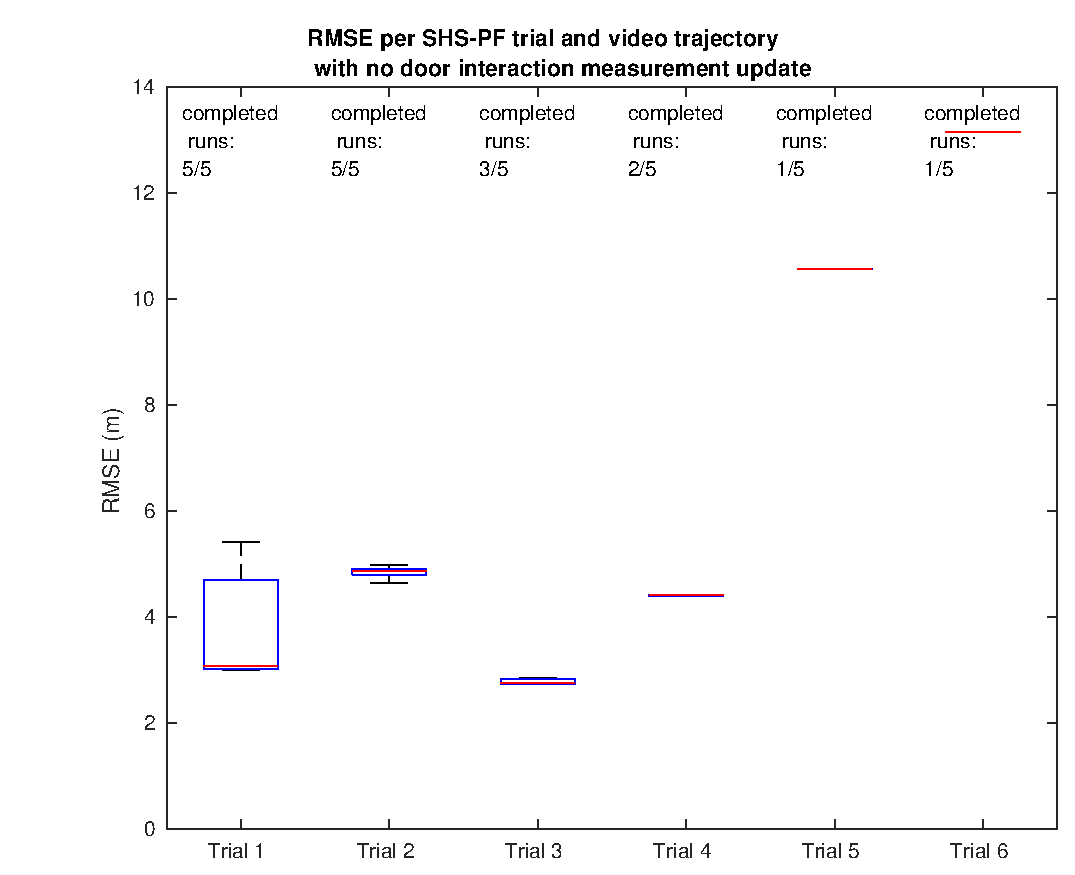
\includegraphics[width=0.7\textwidth]{images/20201129_1438_RMSE_with_no_door_interaction_1}
	\caption[Particle Filter position estimation performance without door interaction]{Particle Filter position estimation performance without door interaction measurement update, 5 iterations per trial. Number under "completed" indicates how many iteration had particles surviving for the whole \ac{SHS}trajectory.}
	\label{fig:pf_boxplot_no_doors}
\end{figure}

The results show that trials 3, and 5 to 7 were unable to complete all iterations. Trial 2 seems to have no difference in performance compared to when activity recognition is used. The RMSE value for trial 1 is similar to that when activity recognition is used, while the spread is larger.
\chapter{Evaluation}

\section{Discussion}
Within the discussion the results of the different \ac{SHS} components and the overall system will be treated, postulating with supporting evidence what may have lead to certain outcomes. Different future avenues are outlined to gain further insight.

\subsection*{Step Detection}
For step detection, the implementation of \cref{algo:step_detect} was compared with that of \citet{Salvi2018}, who had continued the work of \cite{Harle2013}.  \par 
Within the step counting results, there were two observations made. Firstly, the total number of steps counted by both implementations was similar in all carrying modes, many of which had 5\% or less in counting error. There was a large outlier for both cases with the step counting in the back pocket of "user1". Researchers attribute this to the pocket being loose and allowing the phone to rebound when a step was taken \cite{Salvi2018}. This would introduce nefarious components in the accelerometer signal, leading to false positives. \citet{Brajdic2013} encountered similar problems with this carrying position, hypothesizing that the relaxing of the gluteus maximus during locomotion could influence the acceleration trace.\\
The similarity between the two approaches is further underlined by the results in which the time difference between a step detection and its closest ground truth point was calculated. Many detections were within 0.1 seconds from their closest ground truth point. Here the best performing option also changed per carrying mode and person.\par 
Original data was also gathered for step counting and evaluated using the devised method. Here similar results were found to the opensource data. Bad performance in the back pocket was also found, with the best performance being when the smartphone is held in hand. The bad performance in the back pocket further underlines the reliability of step detection in this carrying mode. \par  
The third metric for "unique" step detection was explained and applied, in an attempt to filter out detections detecting the same step. In contrast to the previous metric, this indicated that \cref{algo:step_detect} had more "unique" steps, which are steps closest to a ground truth point, without another detection at the same distance. This would suggest that the current implementation is better at determining the time at which a step occurs. \\
This difference between the two implementations can potentially be explained by the goal and implementation of the \citet{Salvi2018} approach. This research was focused on only \textit{step counting} and did no measurements themselves to determine how close their detections were to the actual steps. Any eventual lag would not affect the step counting performance, as long as the steps are counted. Their android implementation, the output of which was indicated in the validation set, may have had some form of lag. The lag would shift all points, potentially putting them in between step occurrences. This could cause two of them to be in an interval around a ground truth point, which the metric then considers not "unique". \par 

With step detection, the goal was to get similar or better performance than \cite{Salvi2018} . The same parameters found through a variable space search in \cite{Salvi2018}, were used in the step detection method, with the idea that the same performance would be reached. While the results seem to show similar results, it may be worthwhile to run the same variable to check that the parameters are indeed the best for step detection.

\subsection*{Step Length Estimation}
The step length estimation results show that the general linear relationships outlined in \cite{Vezocnik2019} were found, however, the accuracy claimed was not, performing worse than expected. This is most likely caused by the difference in step detection methods, which \cite{Vezocnik2019} does not state explicitly. A similar small scale experiment was performed. Results from this indicate that normal to slow walking worked best with the approach of \cite{Tian2016}, with a tendency to underestimate the distance traveled. \par 

In contrast to the open-source data, the exact number of steps taken for the tunable parameter dataset was known. The number of steps detect was either exactly the same or two steps off. This suggests that the step detection is working correctly and that the methods may be lacking. It may be worthwhile to test the other algorithms outlined by \cite{Vezocnik2019} to see if there are any other differences between the outcomes. 

\newpage


\subsection*{Orientation Estimation}

\begin{itemize}
	\item There is no concrete way with the data available to check how well the EKF estimate is working in comparison to reality. Only comparing to the android system is possible.
	\item trial 3 and trial 6 had the largest yaw difference of the trials. The yaw traces between the android system and EKF can be found in \cref{fig:202011181708yawdifferencebetweenmethods} and \cref{fig:202011181705yawdifferencebetweenmethods}
	\item EKF for trial 6 has a weird jump and slowly gets back to the estimate of the android system. Not clear what is causing this. \textcolor{red}{How should I handle this further?}
	\item for trial 3 there seems to be a slight offset between the orientation estimations.
\end{itemize}

\begin{figure}[H]
	\centering
	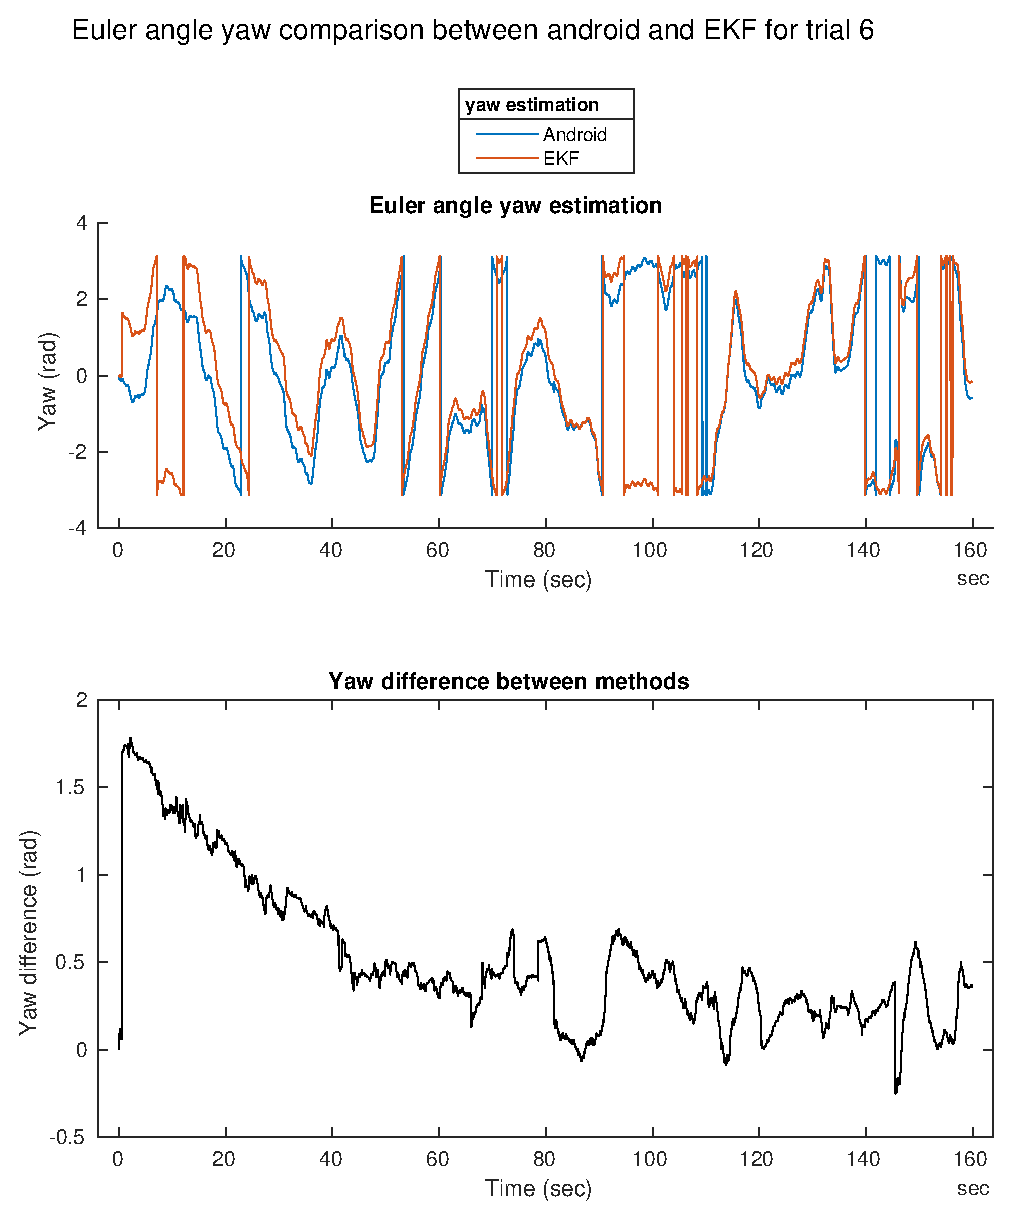
\includegraphics[width=0.7\linewidth]{images/20201118_1708_Yaw_difference_between_methods}
	\caption{}
	\label{fig:202011181708yawdifferencebetweenmethods}
\end{figure}
\begin{figure}[H]
	\centering
	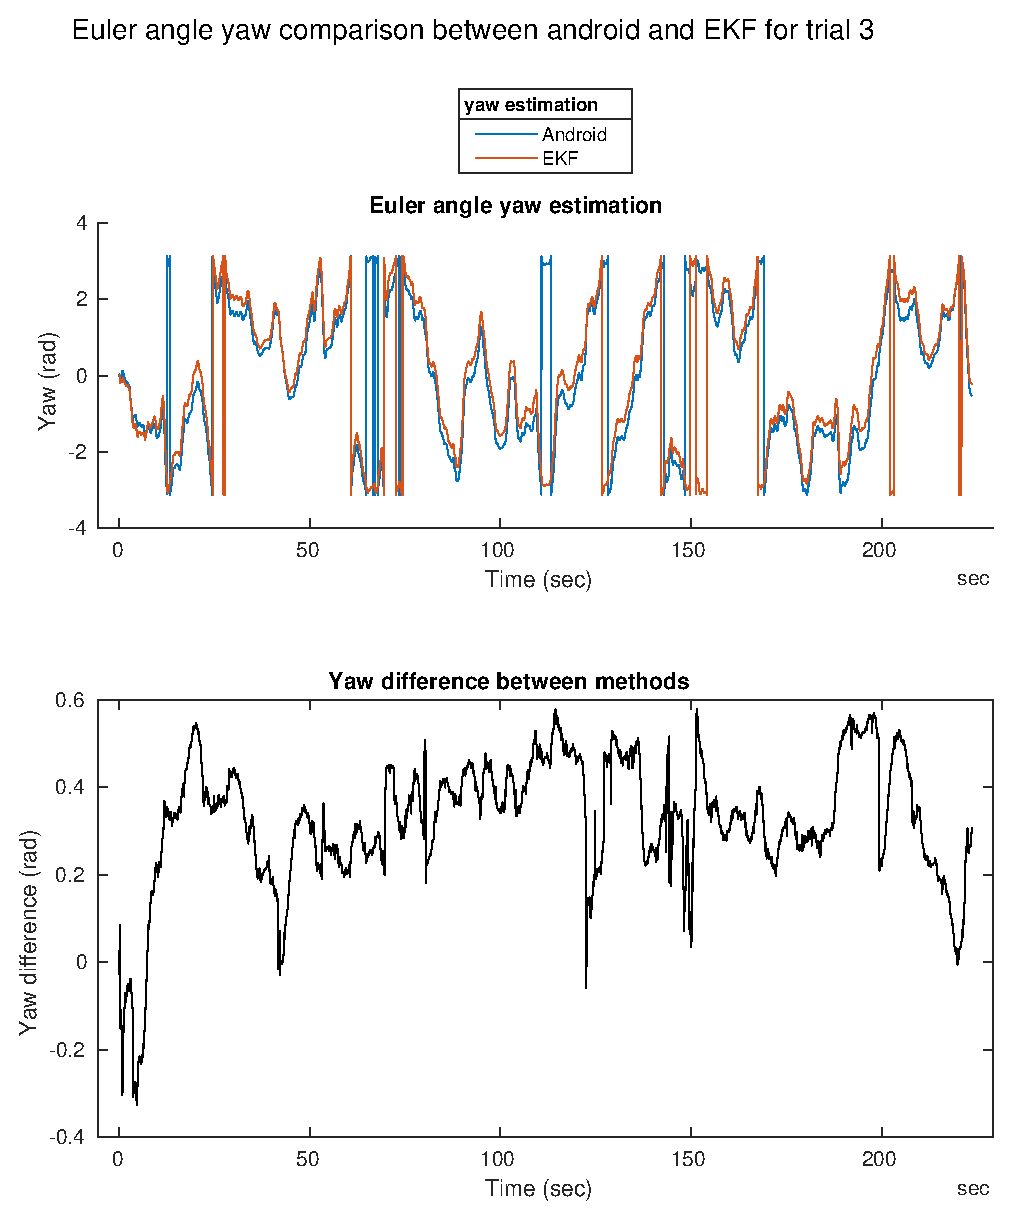
\includegraphics[width=0.7\linewidth]{images/20201118_1705_Yaw_difference_between_methods}
	\caption{}
	\label{fig:202011181705yawdifferencebetweenmethods}
\end{figure}



\newpage
\subsection*{Overall System Performance}

\begin{itemize}
	\item Using door interactions that were manually indicated, 4 out of 6 trials were able to complete all iterations. They do have a difference in median RMSE value and the spread between iterations. The reasoning why this is occurring can be spotted in the trajectories that the particle filter calculates.  
	\item The particle for trial 1 and 2 complete all iterations, it does not follow the complete trajectory. This can be seen in  \cref{fig:shspf_trial1_shs_gt_comparison} where the structure circled in green is circled by the rough estimate but not by the particle filter. For \cref{fig:shspf_trial2_shs_gt_comparison} the particle filter seems to walk too far and is unable to make the correct turn.
	\item trial 3 and 7 are able to follow the whole route. corresponding to lower RMSE values, the outputs are shown in \cref{fig:shspf_trial7_shs_gt_comparison}.
	\item theory that step length estimation is overestimating distance traveled in some cases. This can be caused by turning not having the same displacement as a straight step.
	\item Show a table of the distance walked according to rough video estimate and what the shs estimated.
	\item Comparing the results when activity recognition is not used, the use of activity recognition can potentially improve localization since more trials are able to survive the whole SHS trajectory when it is than when it is not. This is most apparent with trial 7, wherewith activity recognition it is able to complete the whole root, while without it only one iteration survives, which is also has a large error with the video estimate. The results also show that it is not a necessity in some cases to use this form of measurement update, with trial 1 and 2 completing all iterations with similar RMSE values as when AR is used.
	\item When using the AR method outlined in \cref{chap:method}, trial 3 was unable to complete all iterations. The iterations that were completed had a large range of RMSE. This is likely caused by false positives. Plots still need to be made to show this.
\end{itemize}


\begin{figure}[H]
	\centering
	\begin{subfigure}[t]{.45\textwidth}
		\centering
		\begin{tikzpicture}
			\node[anchor=south west,inner sep=0] (image) at (0,0) {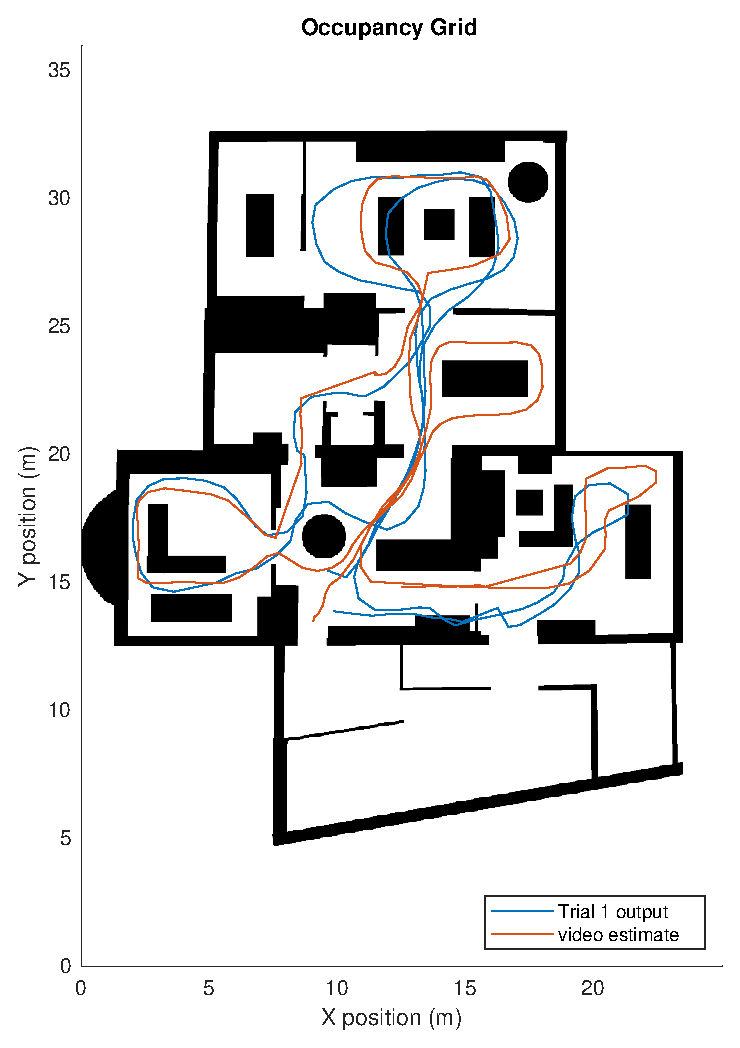
\includegraphics[width=0.9\textwidth]{images/20201118_1900_trial1_output_2}};
			\begin{scope}[x={(image.south east)},y={(image.north west)}]
				\draw[green,ultra thick,rounded corners] (0.6,0.625) rectangle (0.73,0.66);
			\end{scope}
		\end{tikzpicture}		
		\caption{trajectory comparison}
		\label{fig:shspf_trial1_on_map}
	\end{subfigure}
	\begin{subfigure}[t]{.45\textwidth}
		\centering
		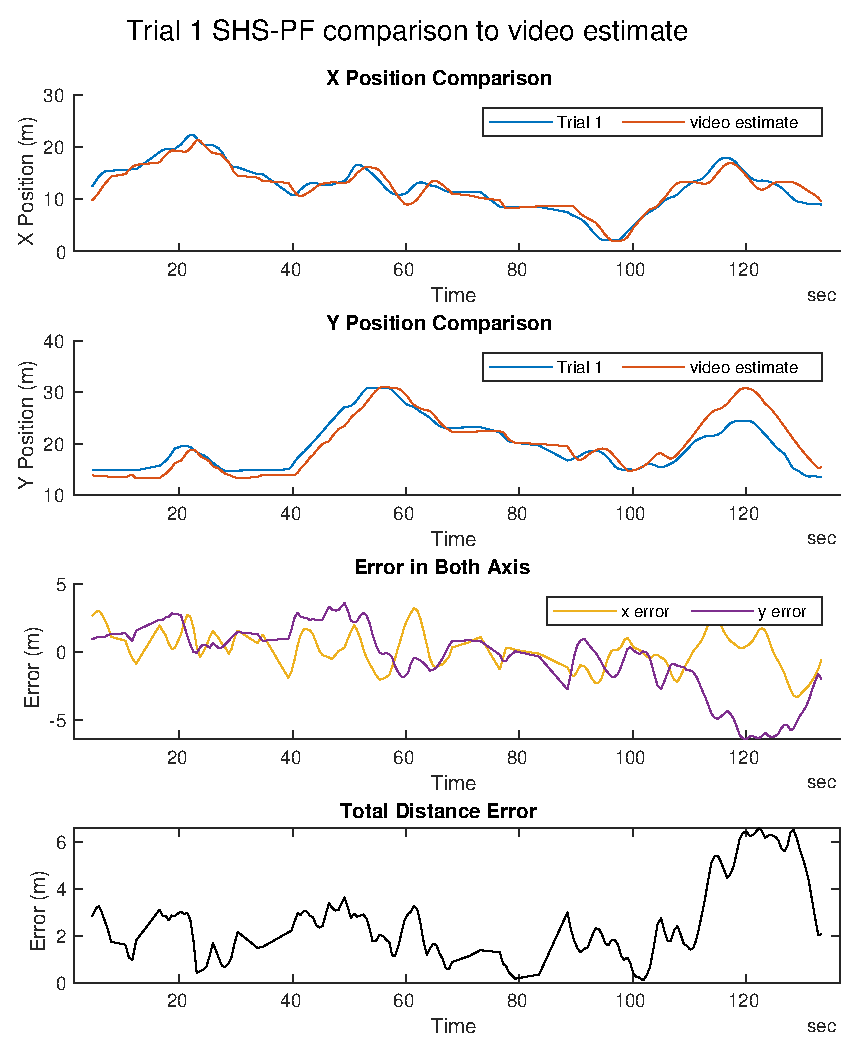
\includegraphics[width=\linewidth]{images/20201118_1900_trial1_output_1}
		\caption{axis comparison}
		\label{fig:shspf_trial1_comparison}
	\end{subfigure}
	\setlength{\belowcaptionskip}{-20pt}
	\caption{SHS-PF comparison of trial 1 with ground truth}
	\label{fig:shspf_trial1_shs_gt_comparison}
\end{figure}
\begin{figure}[H]
	\centering
	\begin{subfigure}[t]{.45\textwidth}
		\centering
		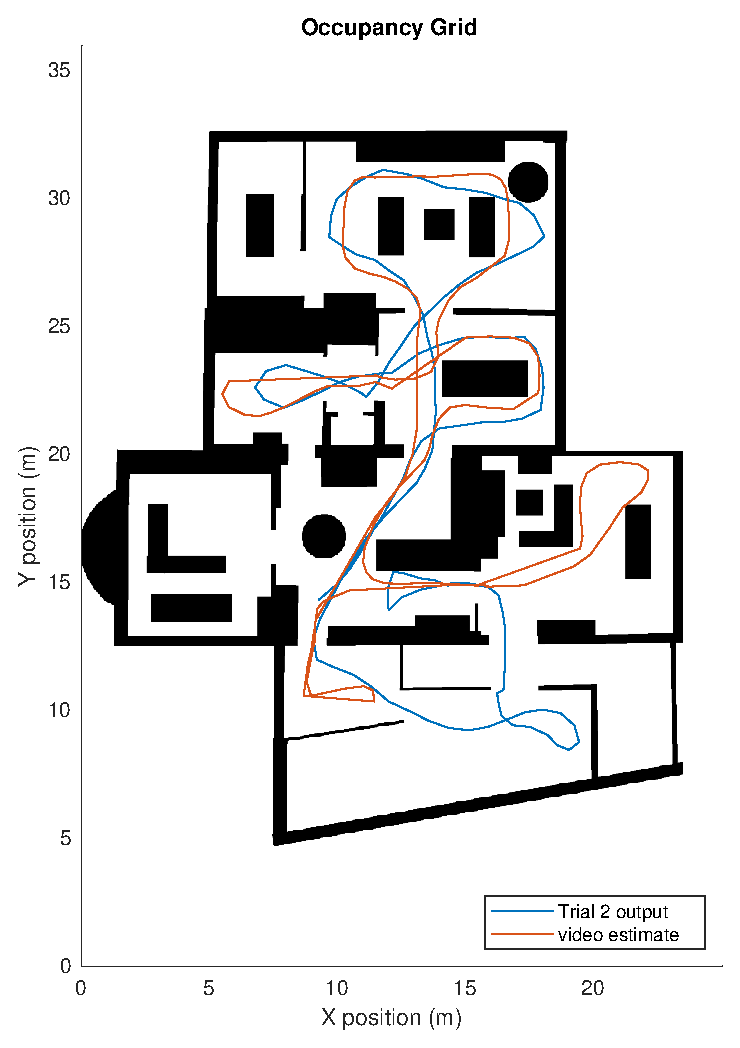
\includegraphics[width=0.9\linewidth]{images/20201118_1902_trial2_output_2}
		\caption{trajectory comparison}
		\label{fig:shspf_trial2_on_map}
	\end{subfigure}
	\begin{subfigure}[t]{.45\textwidth}
		\centering
		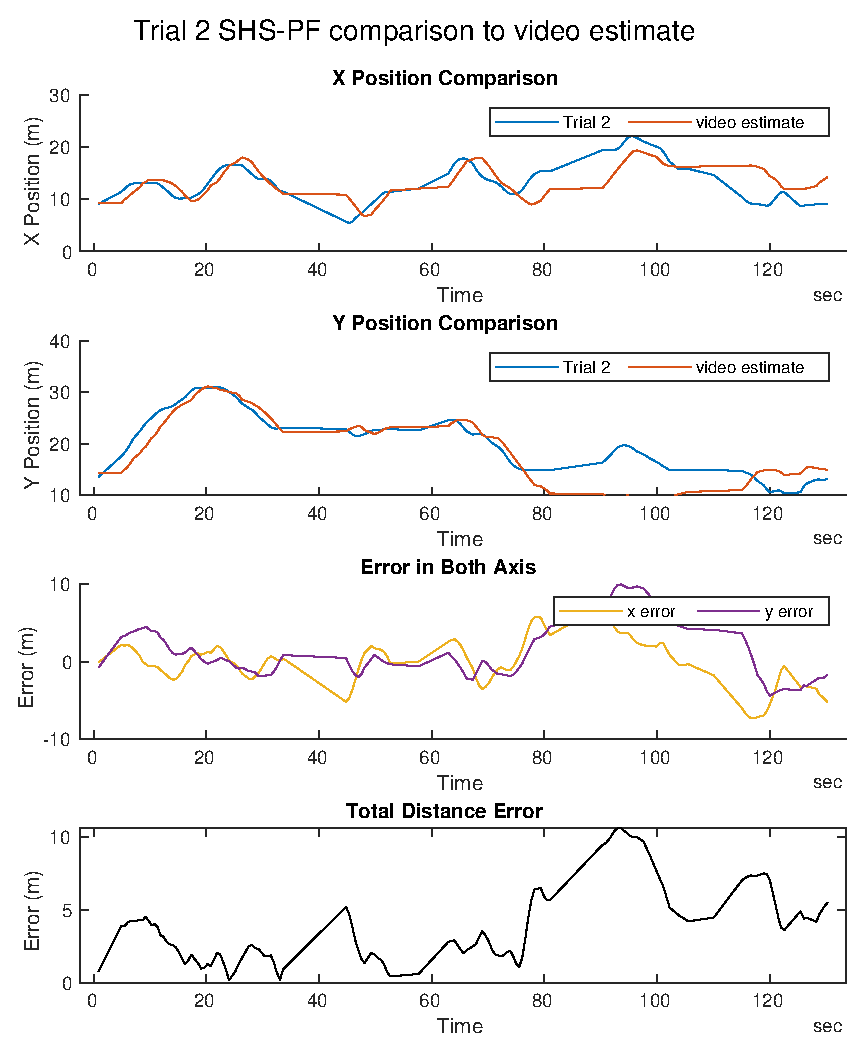
\includegraphics[width=\linewidth]{images/20201118_1902_trial2_output_1}
		\caption{axis comparison}
		\label{fig:shspf_trial2_comparison}
	\end{subfigure}
	\caption{SHS-PF comparison of trial 2 with ground truth}
	\label{fig:shspf_trial2_shs_gt_comparison}
\end{figure}

\begin{figure}[H]
	\centering
	\begin{subfigure}[t]{.45\textwidth}
		\centering
		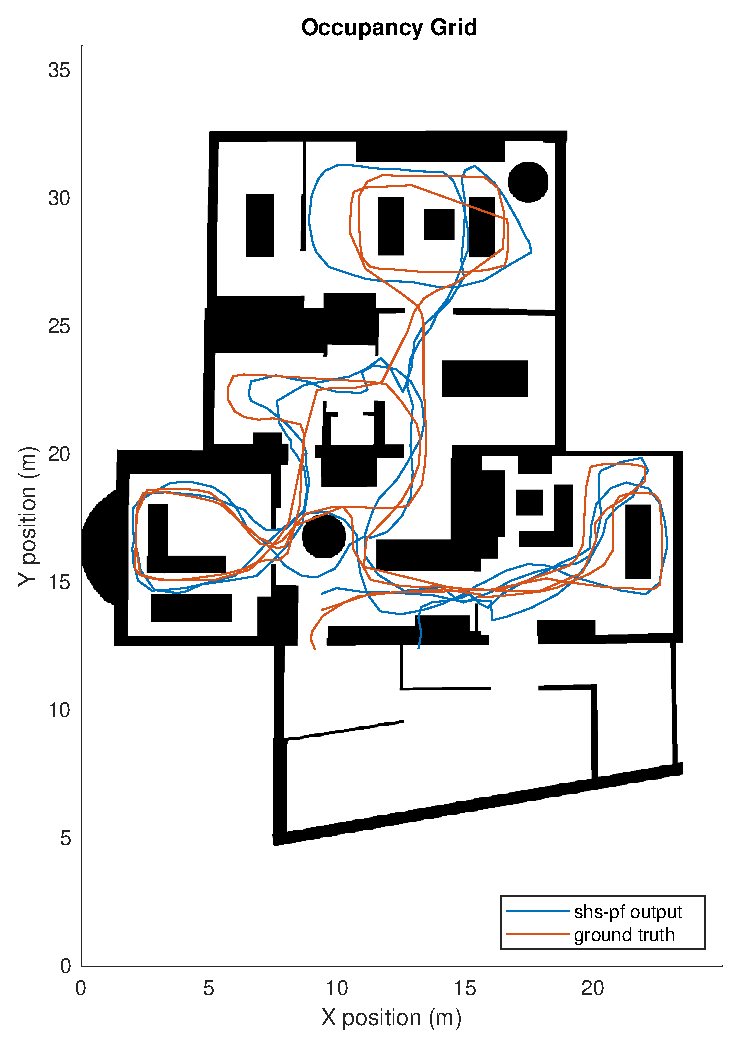
\includegraphics[width=0.9\linewidth]{images/20201029_1804_shs-pf_trial_3_2}
		\caption{trajectory comparison}
		\label{fig:shspf_trial3_on_map}
	\end{subfigure}
	\begin{subfigure}[t]{.45\textwidth}
		\centering
		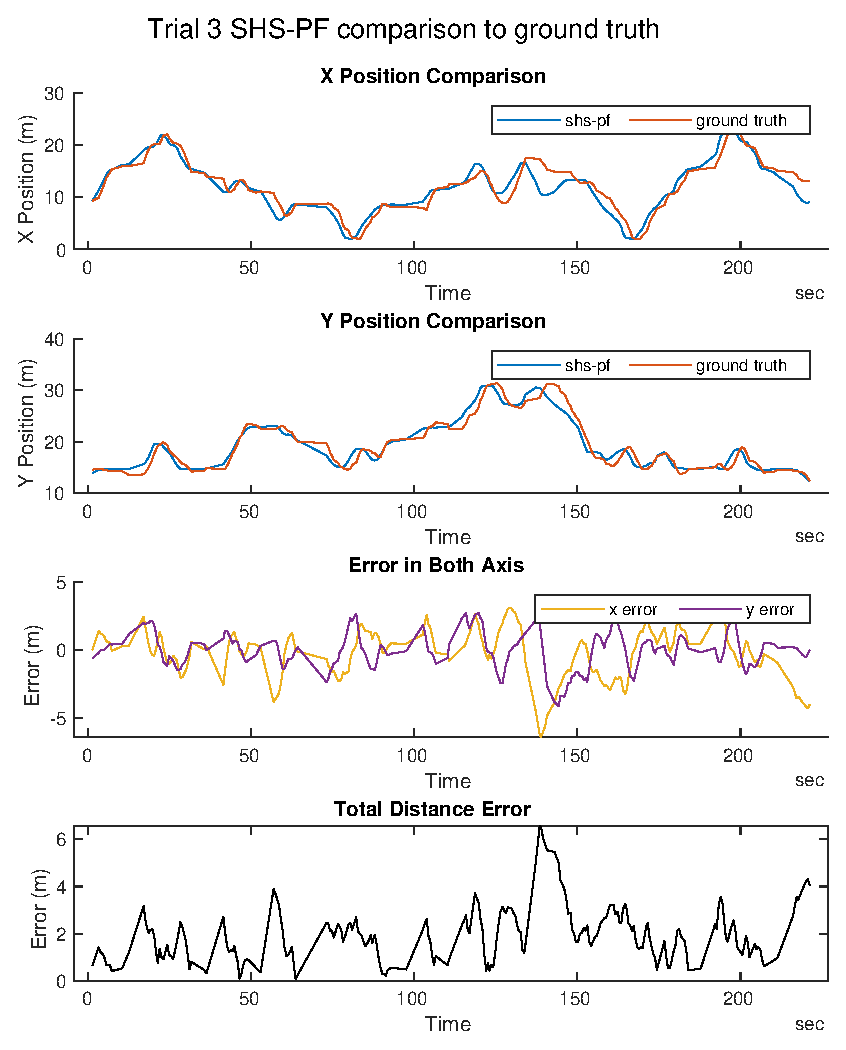
\includegraphics[width=\linewidth]{images/20201029_1804_shs-pf_trial_3_1}
		\caption{axis comparison}
		\label{fig:shspf_trial3_comparison}
	\end{subfigure}
	\caption{SHS-PF comparison of trial 3 with ground truth \textcolor{red}{change legends}}
	\label{fig:shspf_trial3_shs_gt_comparison}
\end{figure}
\begin{figure}[H]
	\centering
	\begin{subfigure}[t]{.45\textwidth}
		\centering
		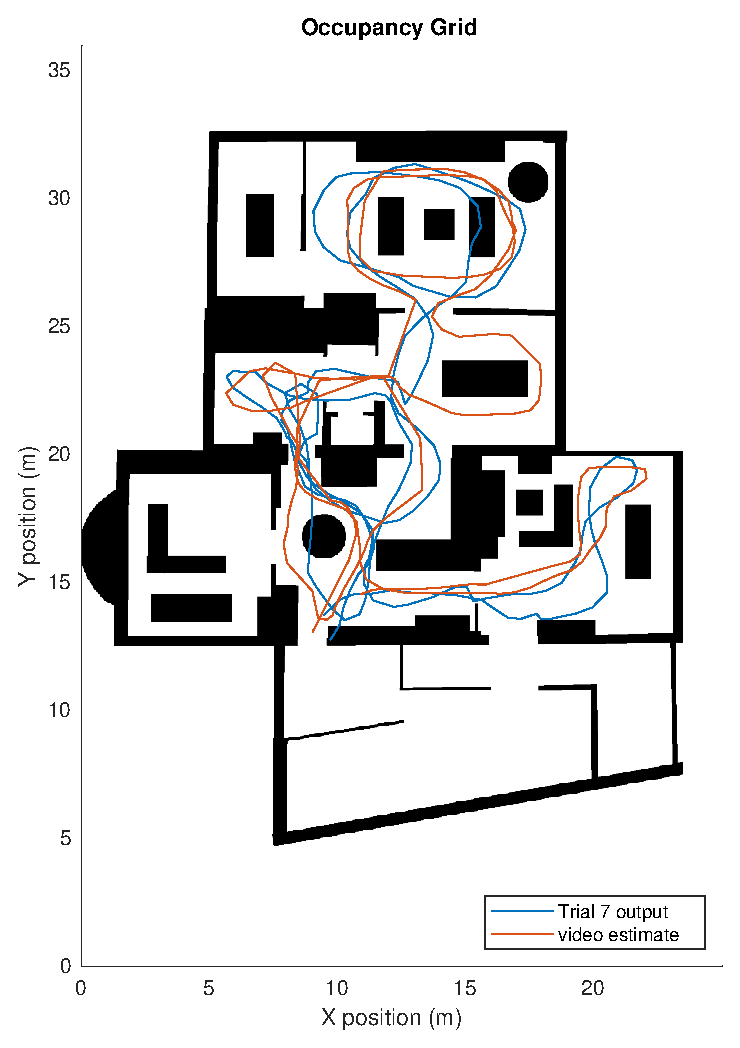
\includegraphics[width=0.9\linewidth]{images/20201118_1908_trial7_output_2}
		\caption{trajectory comparison}
		\label{fig:shspf_trial7_on_map}
	\end{subfigure}
	\begin{subfigure}[t]{.45\textwidth}
		\centering
		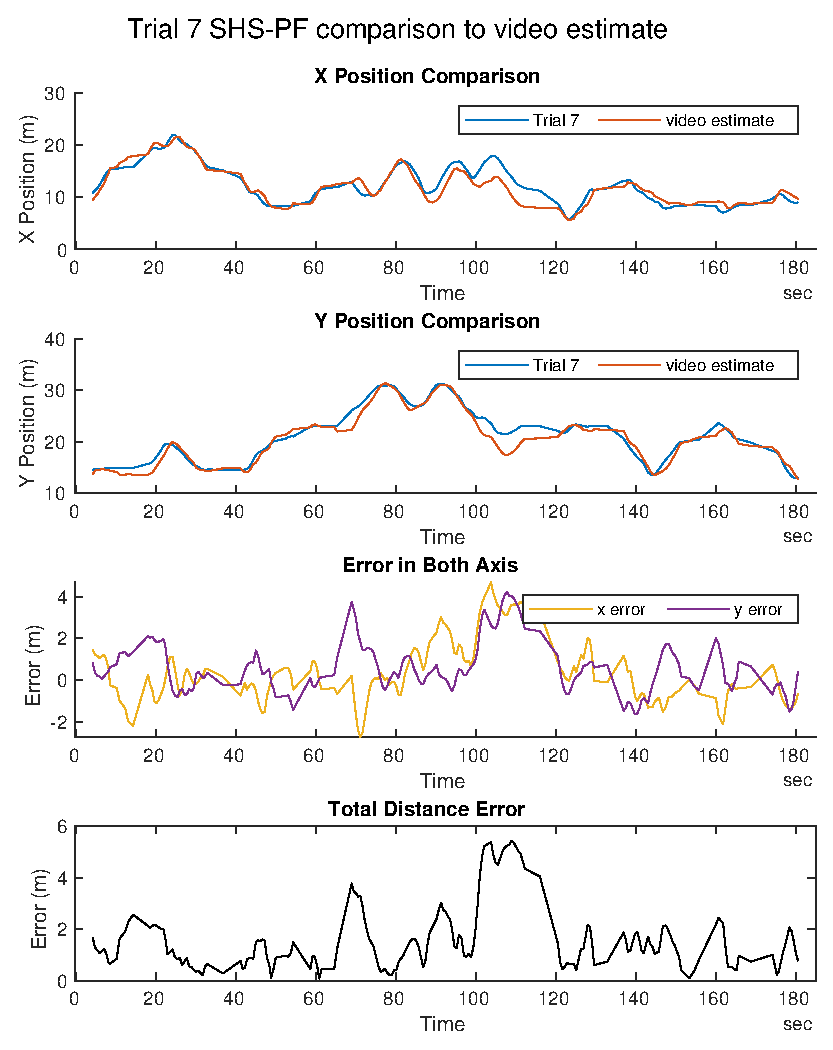
\includegraphics[width=\linewidth]{images/20201118_1908_trial7_output_1}
		\caption{axis comparison}
		\label{fig:shspf_trial7_comparison}
	\end{subfigure}
	\caption{SHS-PF comparison of trial 2 with ground truth}
	\label{fig:shspf_trial7_shs_gt_comparison}
\end{figure}
\newpage
\begin{figure}[H]
	\centering
	\begin{minipage}{.45\textwidth}
		\centering
		\includegraphics[width=\linewidth]{images/20201107_1142_trial_comparison_3}
		\caption{}
		\label{fig:202011071142trialcomparison3}
	\end{minipage}%
	\begin{minipage}{.45\textwidth}
		\centering
		\includegraphics[width=\linewidth]{images/20201107_1142_trial_comparison_2}
		\caption{}
		\label{fig:202011071142trialcomparison2}
	\end{minipage}
\end{figure}


\begin{figure}[H]
	\centering
	\begin{minipage}{.45\textwidth}
		\centering
		\includegraphics[width=\linewidth]{images/20201107_1142_trial_comparison_1}
		\caption{}
		\label{fig:202011071142trialcomparison1}
	\end{minipage}
\end{figure}

\section{Answering Research Questions}

\textcolor{cyan}{this will depend on the the eventual research questions that are found}

\section{Future Work}

{\color{purple}
\textbf{Step detection}
\begin{itemize}
	\item using data from \cite{Salvi2018} determine if parameters found are also the best parameters for the implementation used in this thesis.
	\item Step detection is a form of activity recognition, investigate if other machine learning techniques can perform better  
	\item testing was performed walking on a hard floor and it will be necessary to investigate softer surfaces like carpet or grass.
	\item Determine robustness against more complex movements
\end{itemize}

\textbf{Step length estimation}
\begin{itemize}
	\item generate more first hand data, maybe in a motion capture lab  
	\item use \cite{Bayev2019}, a data set that has recently been made to develop smartphone based pedestrian navigation 
	\item make the assumption that step length is constant and determine effect on performance
	\item when making a turn both feet do not travel the same distance. The inside foot will make a smaller step, while the outer a large one. Determine how turning affects the step length estimation.
\end{itemize}

\textbf{Orientation estimation}
\begin{itemize}
	\item use the method of \cite{Michel2018} to handle magnetic field disturbances
\end{itemize}

\textbf{Step heading estimation}
\begin{itemize}
	\item The testing was limited to one carrying mode, so that the yaw of the device would represent the direction in which the test subject is moving. Step heading estimation will need to be applied in order for the phone to be in other carrying modes.
\end{itemize}

\textbf{Particle filter}
\begin{itemize}
	\item Test without furniture or with a different probability density for furniture
	\item decrease probability close to walls since people do not generally walk close to walls
	\item different representation of map, instead of grid based more node and edge approach. 
	\item be able to detect when moving to a different floor
	\item combine other drift reduction methods
	\item initialize particles over whole map instead of defining a starting point.
	\item find a way to use less particles in order to be implementable on portable device. Above solutions could already help with this.
\end{itemize}

\textbf{Activity Recognition}
\begin{itemize}
	\item Detect more useful activities that can be used as additional particle filter measurement update. For example, climbing stairs for only smartphone sensors, or more intricate activities such as cooking
\end{itemize}

\textbf{Testing}
\begin{itemize}
	\item different building testing. The current contained may different ways of walking around, while other buildings with more corridor structures are more restrictive. Potentially the SHS-PF technique could have better performance in these settings.
	\item better ground truth determination for both positioning and orientation. ORB-SLAM2 was tried but could not get it to work with footage from phone.
	\item online calculation of position on device
	\item test with different people to determine how user sensitive this is.
\end{itemize}}




\chapter{Conclusion}

%
%
%========================== Appendices =======================================
\appendix
%
%
% An Appendix
\chapter{Indoor Localization Experiment}
\label{appendix:shs_experiment}
\textbf{Apparatus}:

\emph{Hardware}:

\begin{itemize}
	\item
	3 Smartphones
	
	\begin{itemize}
		\tightlist
		\item
		Samsung j5 for video recording
		\item
		Iphone for backup orientation estimation and post processing time
		synchronization
		\item
		One Plus Nord for primary orientation estimation and ground truth
		activity recorder
	\end{itemize}
	\item
	1 apple smartwatch
	\item
	Shirt with two breast pockets
	\item
	Indoor test location
\end{itemize}

\emph{Software}:

\begin{itemize}
	\tightlist
	\item
	Iphone and apple watch app
	(\url{https://apps.apple.com/us/app/sensorlog/id388014573\#?platform=appleWatch})
	\item
	Android app for primary sensor recording
	(\url{https://play.google.com/store/apps/details?id=fr.inria.tyrex.senslogs\&hl=en\&gl=US}
	)
\end{itemize}

\textbf{Calibration}:

Calibrate primary estimation sensor (One Plus Nord) just before
experiment, and perform all calibration at the same location within test
location!

\begin{itemize}
	\item
	\emph{Magnetometer}:
	
	\begin{itemize}
		\tightlist
		\item
		Stand away from any clear magnetic disturbance 
		\item
		rotate the phone in as many orientations as possible, infinity sign
		is often used
	\end{itemize}
	\item
	\emph{Accelerometer}:
	
	\begin{itemize}
		\tightlist
		\item
		Rotate the phone slowly in as many orientations as possible in
		attempting to be in as many orientations as possible.
	\end{itemize}
	\item
	\emph{Gyroscope / Magnetic North / Noise}
	
	\begin{itemize}
		\item
		Lay the phone horizontally and start recording while stationary
	\end{itemize}
\end{itemize}

\textbf{Preparation}:

\begin{enumerate}
	\def\labelenumi{\arabic{enumi}.}
	\tightlist
	\item
	Calibrate One Plus Nord with the calibration method outlined above
	\item
	Determine with which hand you will hold the phone, strap the
	smartwatch to the other hand
	\item
	Ensure that all doors in test location are closed
	\item
	Define start location within test location and record it
\end{enumerate}

\textbf{Testing}:

For \emph{each test run} perform the following steps:

\begin{enumerate}
	\def\labelenumi{\arabic{enumi}.}
	\tightlist
	\item
	Go to start location
	\item
	Start sensor recording on smartwatch and iPhone
	\item
	place iPhone in one of the breast pockets of the shirt
	\item
	Start a video recording on the Samsung phone and place it in the other
	breast pocket, making sure that the lens is not covered and can see
	what is in front of the torso of the test subject, hence also what
	direction is being moved in.
	\item
	Start sensor recording on One Plus Nord, logging the uncalibrated
	accelerometer, gyroscope, and magnetometer. Also record the rotation
	vector that the phone records. This is shown in illustration 1.
	\item
	Walk around test location as naturally as possible, holding the One
	Plus Nord in front of you with the screen point up. Try and keep this
	phone orientation as best as possible.
	\item
	Walk to doors and open them using the arm that has the smartwatch on
	it. When touching a door handle click the button in the android app
	that records the time stamp as shown in illustration 2. Close the door
	behind you, so that it can potentially be opened again later.
	\item
	After walking for around 3 minutes, return to start location
	\item
	Stop recording of sensor and video on all devices
	\item
	export the data (film and sensor) from all 3 devices to the same
	folder, making it clear which trail it was
\end{enumerate}

\textbf{Pictures}:
\begin{figure}[H]
	\centering
	\begin{subfigure}[t]{.45\textwidth}
		\centering
		\includegraphics[width=0.6\linewidth]{images/recording_setting}
		\caption{Recording settings}
		\label{fig:recording_setting}
	\end{subfigure}
	\begin{subfigure}[t]{.45\textwidth}
		\centering
		\includegraphics[width=0.7\linewidth]{images/recording_timestamp_button}
		\caption{Record timestamp button}
		\label{fig:recording_timestamp_button}
	\end{subfigure}
\caption{Indoor experiment android app configuration and button}
\end{figure}


\textbf{Postprocessing}

\begin{enumerate}
	\def\labelenumi{\arabic{enumi}.}
	\tightlist
	\item
	Calibrate walking around imu sensor data using calibration data
	\item
	Run calibrated walking around data through orientation estimation
	algorithm
	\item
	Compare result with orientation estimation made by the system and
	maybe even with the iphone 
	\item
	Determine steps and subsequent step length 
	\item
	Combine orientation information and step information to generate an
	estimated trajectory
	\item
	Use this estimated trajectory as input for the particle filter
	\item
	Using the video recording made during testing, manually indicate per
	step where on the blueprint you are. This will be used to determine
	the performance of the estimate of the SHS system. 
\end{enumerate}

\chapter{Indoor Experiment Results}

\section{SHS-PF parameter search}
\begin{figure}[H]
	\centering
	\includegraphics[width=0.7\linewidth]{images/20201107_1312_orientation_std_0_2}
	\caption{}
	\label{fig:202011071312orientationstd02}
\end{figure}
\begin{figure}[H]
	\centering
	\includegraphics[width=0.7\linewidth]{images/20201107_1311_orientation_std_0_2}
	\caption{}
	\label{fig:202011071311orientationstd02}
\end{figure}

\section{SHS-PF estimator comparison}
\begin{figure}[H]
	\centering
	\includegraphics[width=0.5\linewidth]{images/20201108_1559_lopen1_1_estimation_comparison}
	\caption{}
	\label{fig:202011081559lopen11estimationcomparison}
\end{figure}
\begin{figure}[H]
	\centering
	\includegraphics[width=0.5\linewidth]{images/20201108_1601_lopen1_3_estimation_comparison}
	\caption{}
	\label{fig:202011081601lopen13estimationcomparison}
\end{figure}
\begin{figure}[H]
	\centering
	\includegraphics[width=0.5\linewidth]{images/20201108_1559_lopen1_2_estimation_comparison}
	\caption{}
	\label{fig:202011081559lopen12estimationcomparison}
\end{figure}




\section{SHS-PF performance}
\label{app:SHS-PF trials}




\chapter{Experiment trials visualization}
\subsection{Perfect activity recognition}
\newpage
\subsubsection{Trial 1}

\begin{figure}[H]
	\centering
	\begin{subfigure}[t]{.45\textwidth}
		\centering
		\includegraphics[width=0.9\linewidth]{images/20201029_1040_trial1_shs_1}
		\caption{trajectory comparison}
		\label{fig:trial1_on_map}
	\end{subfigure}
	\begin{subfigure}[t]{.45\textwidth}
		\centering
		\includegraphics[width=\linewidth]{images/20201029_1040_trial1_shs_2}
		\caption{axis comparison}
		\label{fig:trial1_comparison}
	\end{subfigure}
	\caption{Qualitative SHS comparison of trial 1 with ground truth}
	\label{fig:trial1_shs_gt_comparison}
\end{figure}

\subsubsection{Trial 2}

\begin{figure}[H]
	\centering
	\begin{subfigure}[t]{.45\textwidth}
		\centering
		\includegraphics[width=0.9\linewidth]{images/20201029_1042_trial2_shs_1}
		\caption{trajectory comparison}
		\label{fig:trial2_on_map}
	\end{subfigure}
	\begin{subfigure}[t]{.45\textwidth}
		\centering
		\includegraphics[width=\linewidth]{images/20201029_1042_trial2_shs_2}
		\caption{axis comparison}
		\label{fig:trial2_comparison}
	\end{subfigure}
\setlength{\belowcaptionskip}{-20pt}
	\caption{Qualitative SHS comparison of trial 2 with ground truth}
	\label{fig:trial2_shs_gt_comparison}
\end{figure}

\subsubsection{Trial 3}



%%
% Another appendix chapter
\chapter{Yet Another Appendix}


\section{Test Section (Again?)}

Ok, all is well.


%========================== Back matter ======================================
\backmatter
%
% Bibliography

\bibliography{Manual_Bibliography.bib,Thesis_Bibliography.bib,Literature_Review_Bibliography.bib}
\bibliographystyle{plainnat}      % This style puts references in order of appearance
%\bibliographystyle{plain}      % This style puts references in alphabetic order
%\printbib{Thesis_Bibliography.bib}
%
%
% Glossary
\chapter{Glossary} %
%
\printacronyms
\begin{acronym}[\hspace{0.8in}] % 0.8in is also used by the nomenclature

	\acro{3mE}[3\textlarger{m}E]{Mechanical, Maritime and Materials Engineering}%

	\acro{AMS}{American Mathematical Society}%

	\acro{DCSC}{Delft Center for Systems and Control}%

	\acro{TU}[TU D\textlarger{elft}]{Delft University of Technology}%

	\acro{PDR}{Pedestrian Dead Reckoning}%

	\acro{SHS}{Step and Heading System}%

	\acro{IMU}{Inertial Measurement Unit}%

	\acro{ZUPT}{Zero Velocity Update}%

	\acro{DTW}{Dynamic Time Warping}%

	\acro{NASC}{Normalized Auto-correlation based Step Counting}

	\acro{INS}{Inertial Navigation System}

	\acro{HMM}{Hidden Markov Model}

	\acro{MEMS}{Micro-Electromechanical Systems}

	\acro{COM}{Center of Mass}

	\acro{EKF}{Extended Kalman Filter}

	\acro{PCA}{Principal Component Analysis}

	\acro{FLAM}{Forward and Lateral Accelerations modeling}

	\acro{FIS}{Frequency analysis of Inertial Signals}

	\acro{SLAM}{Simultaneous Localization and Mapping}

	\acro{SVM}{Support Vector Machine}

	\acro{DT}{Decision Tree}

\end{acronym}%
%
%
% Nomenclature
\printnomencl%
%
% Index
\cleardoublepage
\printindex

\end{document}
